\chapter[EKSPERIMEN]{Eksperimen}
\label{chap:eksperimen}

Bab ini memaparkan bagaimana eksperimen dirancang, dijalankan, dan dianalisis.
Pembahasan mencakup dua kasus penggunaan, yaitu \emph{User Manual} dan kasus hukum. Untuk
masing-masing \emph{use case}, bab ini menyajikan \emph{dataset}, konfigurasi eksperimen, serta
hasil pengukurannya.

\section{Lingkungan Eksperimen}
\label{sec:lingkungan-eksperimen}

Eksperimen dijalankan pada perangkat keras dan perangkat lunak yang mendukung
seluruh subsistem pemrosesan dan pengukuran. Spesifikasinya disajikan pada
Tabel~\ref{tab:lingkungan-eksperimen}.

\begin{table}[H]
  \centering
    \scriptsize
    \renewcommand{\arraystretch}{0.9}
  \caption{Spesifikasi lingkungan eksperimen}
  \label{tab:lingkungan-eksperimen}
  \begin{tabularx}{\textwidth}{@{}>{\RaggedRight\arraybackslash}p{3.4cm}>{\RaggedRight\arraybackslash}X@{}}
    \toprule
    \textbf{Komponen} & \textbf{Spesifikasi} \\
    \midrule
    Prosesor & Intel Core Ultra 9 185H, 16 \emph{core} dan 22 \emph{logical processor}, arsitektur x86-64 \\
    Memori & 32 GB RAM \\
    Perangkat grafis & Intel Arc Graphics terintegrasi. \emph{Embedding} menggunakan distribusi \emph{PyTorch} CPU tanpa CUDA \\
    Sistem operasi & \emph{Ubuntu} 26.04 LTS, kernel \emph{Linux} 7.0.0-30-generic \\
    Kontainer & \emph{Docker} 29.1.3 dan \emph{Docker Compose} 2.40.3 \\
    Bahasa dan \emph{runtime} & \emph{Python} 3.13 pada Debian Bookworm Slim. Pengelolaan \emph{dependency} dilakukan dengan \code{uv} 0.9.2 \\
    \emph{Framework} aplikasi & FastAPI, Pydantic, SQLAlchemy, dan \emph{worker} asinkron berbasis \code{aio-pika} \\
    Infrastruktur data & \emph{PostgreSQL} 16, \emph{object storage}, \emph{RabbitMQ} 3.13, \emph{OpenSearch} 3.3.0, dan \emph{Neo4j} 5.26 \\
    \emph{Model embedding} & BAAI/\emph{BGE-M3} \\
    \bottomrule
  \end{tabularx}
\end{table}

Semua konfigurasi menggunakan \emph{API} dan \emph{worker} dengan jumlah serta konfigurasi yang
sama. Infrastruktur dijaga setara pada setiap konfigurasi sehingga hasil dapat dibandingkan
secara adil dan perubahan yang diamati dapat dikaitkan dengan komponen yang diuji.

\section{Eksperimen pada \emph{Use Case} \emph{User Manual}}
\label{sec:eksperimen-user-manual}

\subsection{\emph{Dataset} Eksperimen}
\label{subsec:dataset-user-manual}

\emph{Dataset} \emph{User Manual} dibangun menggunakan sembilan manual produk Netgear yang
tersedia, sebagaimana diringkas pada Tabel~\ref{tab:customer-corpus-coverage}.

\begin{table}[H]
\centering
\small
\caption{Cakupan dokumen pada \emph{dataset} \emph{User Manual}}
\label{tab:customer-corpus-coverage}
\begin{tabularx}{0.75\textwidth}{@{}>{\RaggedRight\arraybackslash}X r@{}}
\toprule
\textbf{\emph{Model} produk} & \textbf{Halaman}\\
\midrule
CM2000 & 26\\
LM1200 & 105\\
R6350 & 204\\
R7000 & 186\\
RAX120 & 175\\
RAX50 & 160\\
RAXE500 & 169\\
RBK852 & 161\\
XR500 & 214\\
\midrule
\textbf{Total} & \textbf{1.400}\\
\bottomrule
\end{tabularx}
\end{table}

\subsubsection{Pembentukan \emph{Dataset} Pertanyaan dan Jawaban}
\label{subsubsec:user-manual-question-dataset}

Subbab ini menjelaskan bagaimana cara membuat \emph{dataset} pertanyaan dan jawaban acuan
yang digunakan sebagai dasar eksperimen. Prosesnya terdiri atas empat tahap berikut.

\begin{enumerate}[leftmargin=*, itemsep=0.25em]
  \item \textbf{Menetapkan sumber dan kandidat.} Sembilan manual Netgear dipakai sebagai korpus.
  \emph{Parser} membentuk judul dan blok teks berdasarkan \emph{outline} pada setiap dokumen. Bagian
  akhir \emph{outline} yang tidak memiliki struktur turunan digunakan sebagai simpul akhir. Blok teks
  terakhir pada setiap bagian tersebut yang memiliki teks langsung kemudian dijadikan kandidat konteks.
  Pemilihannya menggunakan \emph{stratified sampling} berdasarkan kombinasi dokumen dan kelompok
  persentil halaman P1--P5. Setiap manual mendapat alokasi \emph{minimum}, sedangkan alokasi sisanya mengikuti
  jumlah halaman, kemudian pengambilan dilakukan secara acak-terkendali dengan \emph{seed} yang sama.
  \item \textbf{Mengisi slot pertanyaan dan bahasa.} Kandidat konteks dipakai untuk membekukan
  100 \emph{slot} pertanyaan, dengan \emph{seed} \texttt{20260831} agar seluruh dokumen serta
  posisi halaman tetap terwakili. Istilah \emph{slot} di sini berarti satu posisi yang harus diisi
  oleh satu pertanyaan dan satu jawaban acuan. Setiap slot kemudian diberi satu pertanyaan bahasa Inggris dan
  satu pertanyaan bahasa Indonesia. Dengan demikian, \emph{dataset} berisi 200 baris pertanyaan,
  yaitu 100 pasangan slot berbahasa Inggris--Indonesia. Setiap slot juga diberi satu kategori
  berdasarkan fokus informasi yang diminta, yaitu fakta dan spesifikasi, penyiapan dan konfigurasi,
  pemecahan masalah dan diagnosis, atau fitur, keamanan, pemeliharaan, dan keterbatasan.
  \item \textbf{Menyiapkan konteks per slot.} Untuk setiap slot dibuat satu paket konteks yang
  menunjuk tepat satu \emph{leaf outline} dan satu blok teks sumber. Paket menyimpan ID dokumen,
  halaman, urutan blok, serta \texttt{source\_block\_id}. Paket yang sama dipakai oleh dua varian bahasa
  dari slot tersebut. \emph{Model} hanya menggunakan paket ini untuk menyusun pertanyaan serta jawaban
  acuan, sedangkan eksperimen \emph{retrieval} tetap mencocokkan ID blok pada konfigurasi yang digunakan.
  \item \textbf{Membentuk \emph{dataset}.} Setelah konteks tersedia, konteks tersebut diberikan kepada
  \emph{model} \texttt{openai/gpt-5.6-luna}. \emph{Model} menyusun pertanyaan dan jawaban berdasarkan konteks yang menjadi
  acuan untuk satu \emph{slot}. Selanjutnya, \emph{model} menandai ID blok pada konteks sebagai
  \emph{context reference}. ID ini digunakan dalam metrik eksperimen pada proses \emph{retrieval}.
\end{enumerate}

\subsubsection{Distribusi \emph{Dataset}}
\label{subsubsec:user-manual-dataset-distribution}

Distribusi pertanyaan dibuat seimbang antara bahasa Inggris dan bahasa Indonesia. Setiap pasangan
bahasa berasal dari \emph{slot} dan \emph{context reference} yang sama, perbedaannya hanya pada
bahasa pertanyaan. Lokasi konteks dipilih dari seluruh dokumen dan disebar berdasarkan posisi
halaman relatif.

Gambar~\ref{fig:customer-question-count-by-document} memperlihatkan jumlah pertanyaan
bahasa Inggris dan Indonesia yang sama pada setiap dokumen untuk \emph{use case} \emph{User Manual}.

\begin{figure}[H]
\centering
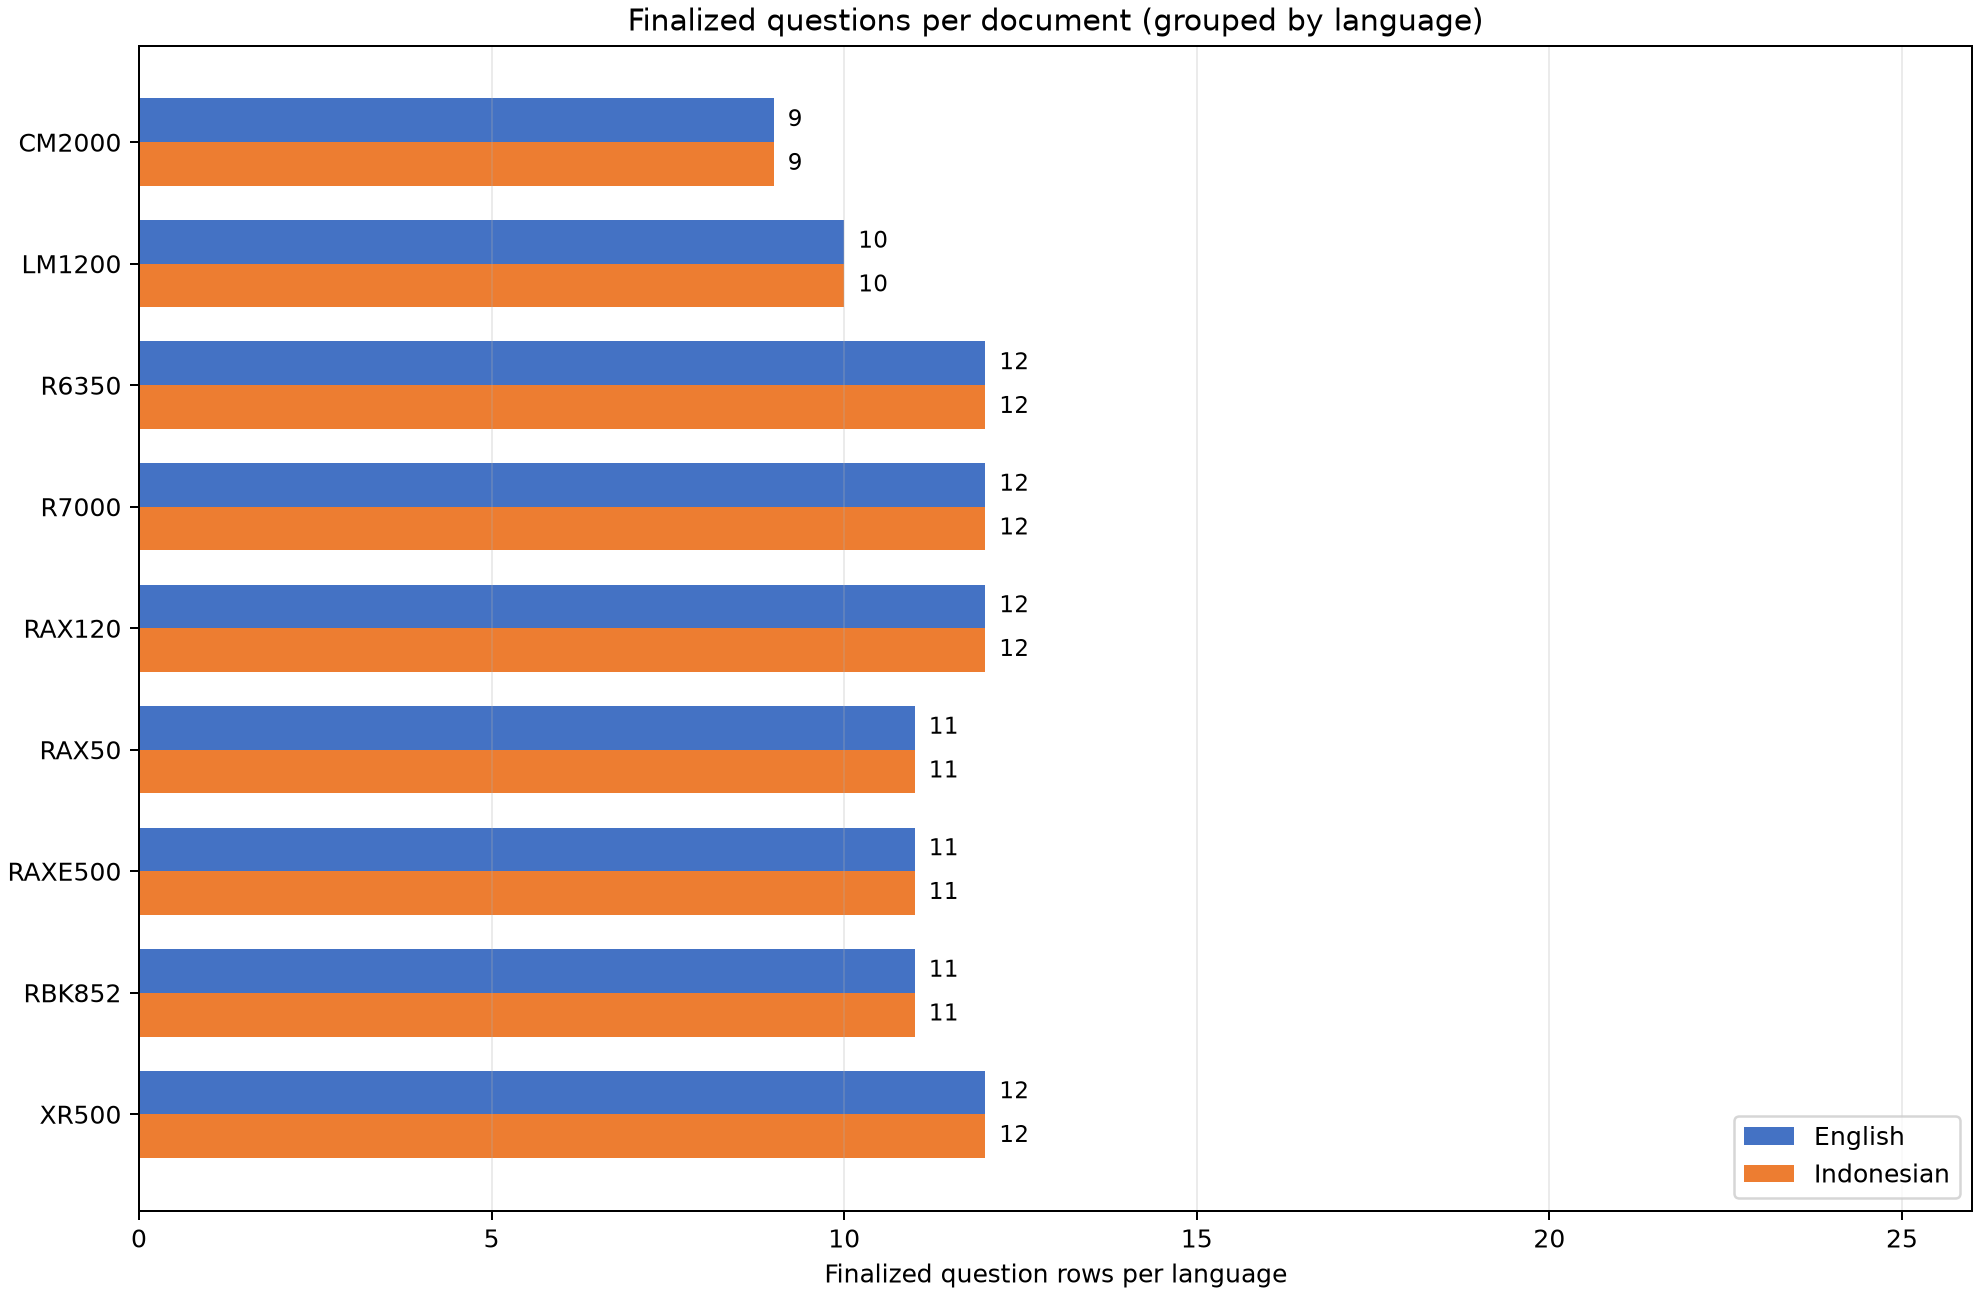
\includegraphics[width=\textwidth,height=0.55\textheight,keepaspectratio]{images/experiments/customer_service_revision/final_eda/question-count-by-document.png}
\caption{Distribusi jumlah pertanyaan per dokumen dan bahasa}
\label{fig:customer-question-count-by-document}
\end{figure}

Gambar~\ref{fig:customer-question-category-distribution} merangkum kategori pertanyaan pada
setiap produk. Total tiap kategori seimbang, sedangkan komposisi produk mengikuti isi manual.
Batang Inggris dan Indonesia sama panjang sehingga keseimbangan bahasa tetap terlihat.

\begin{figure}[H]
\centering
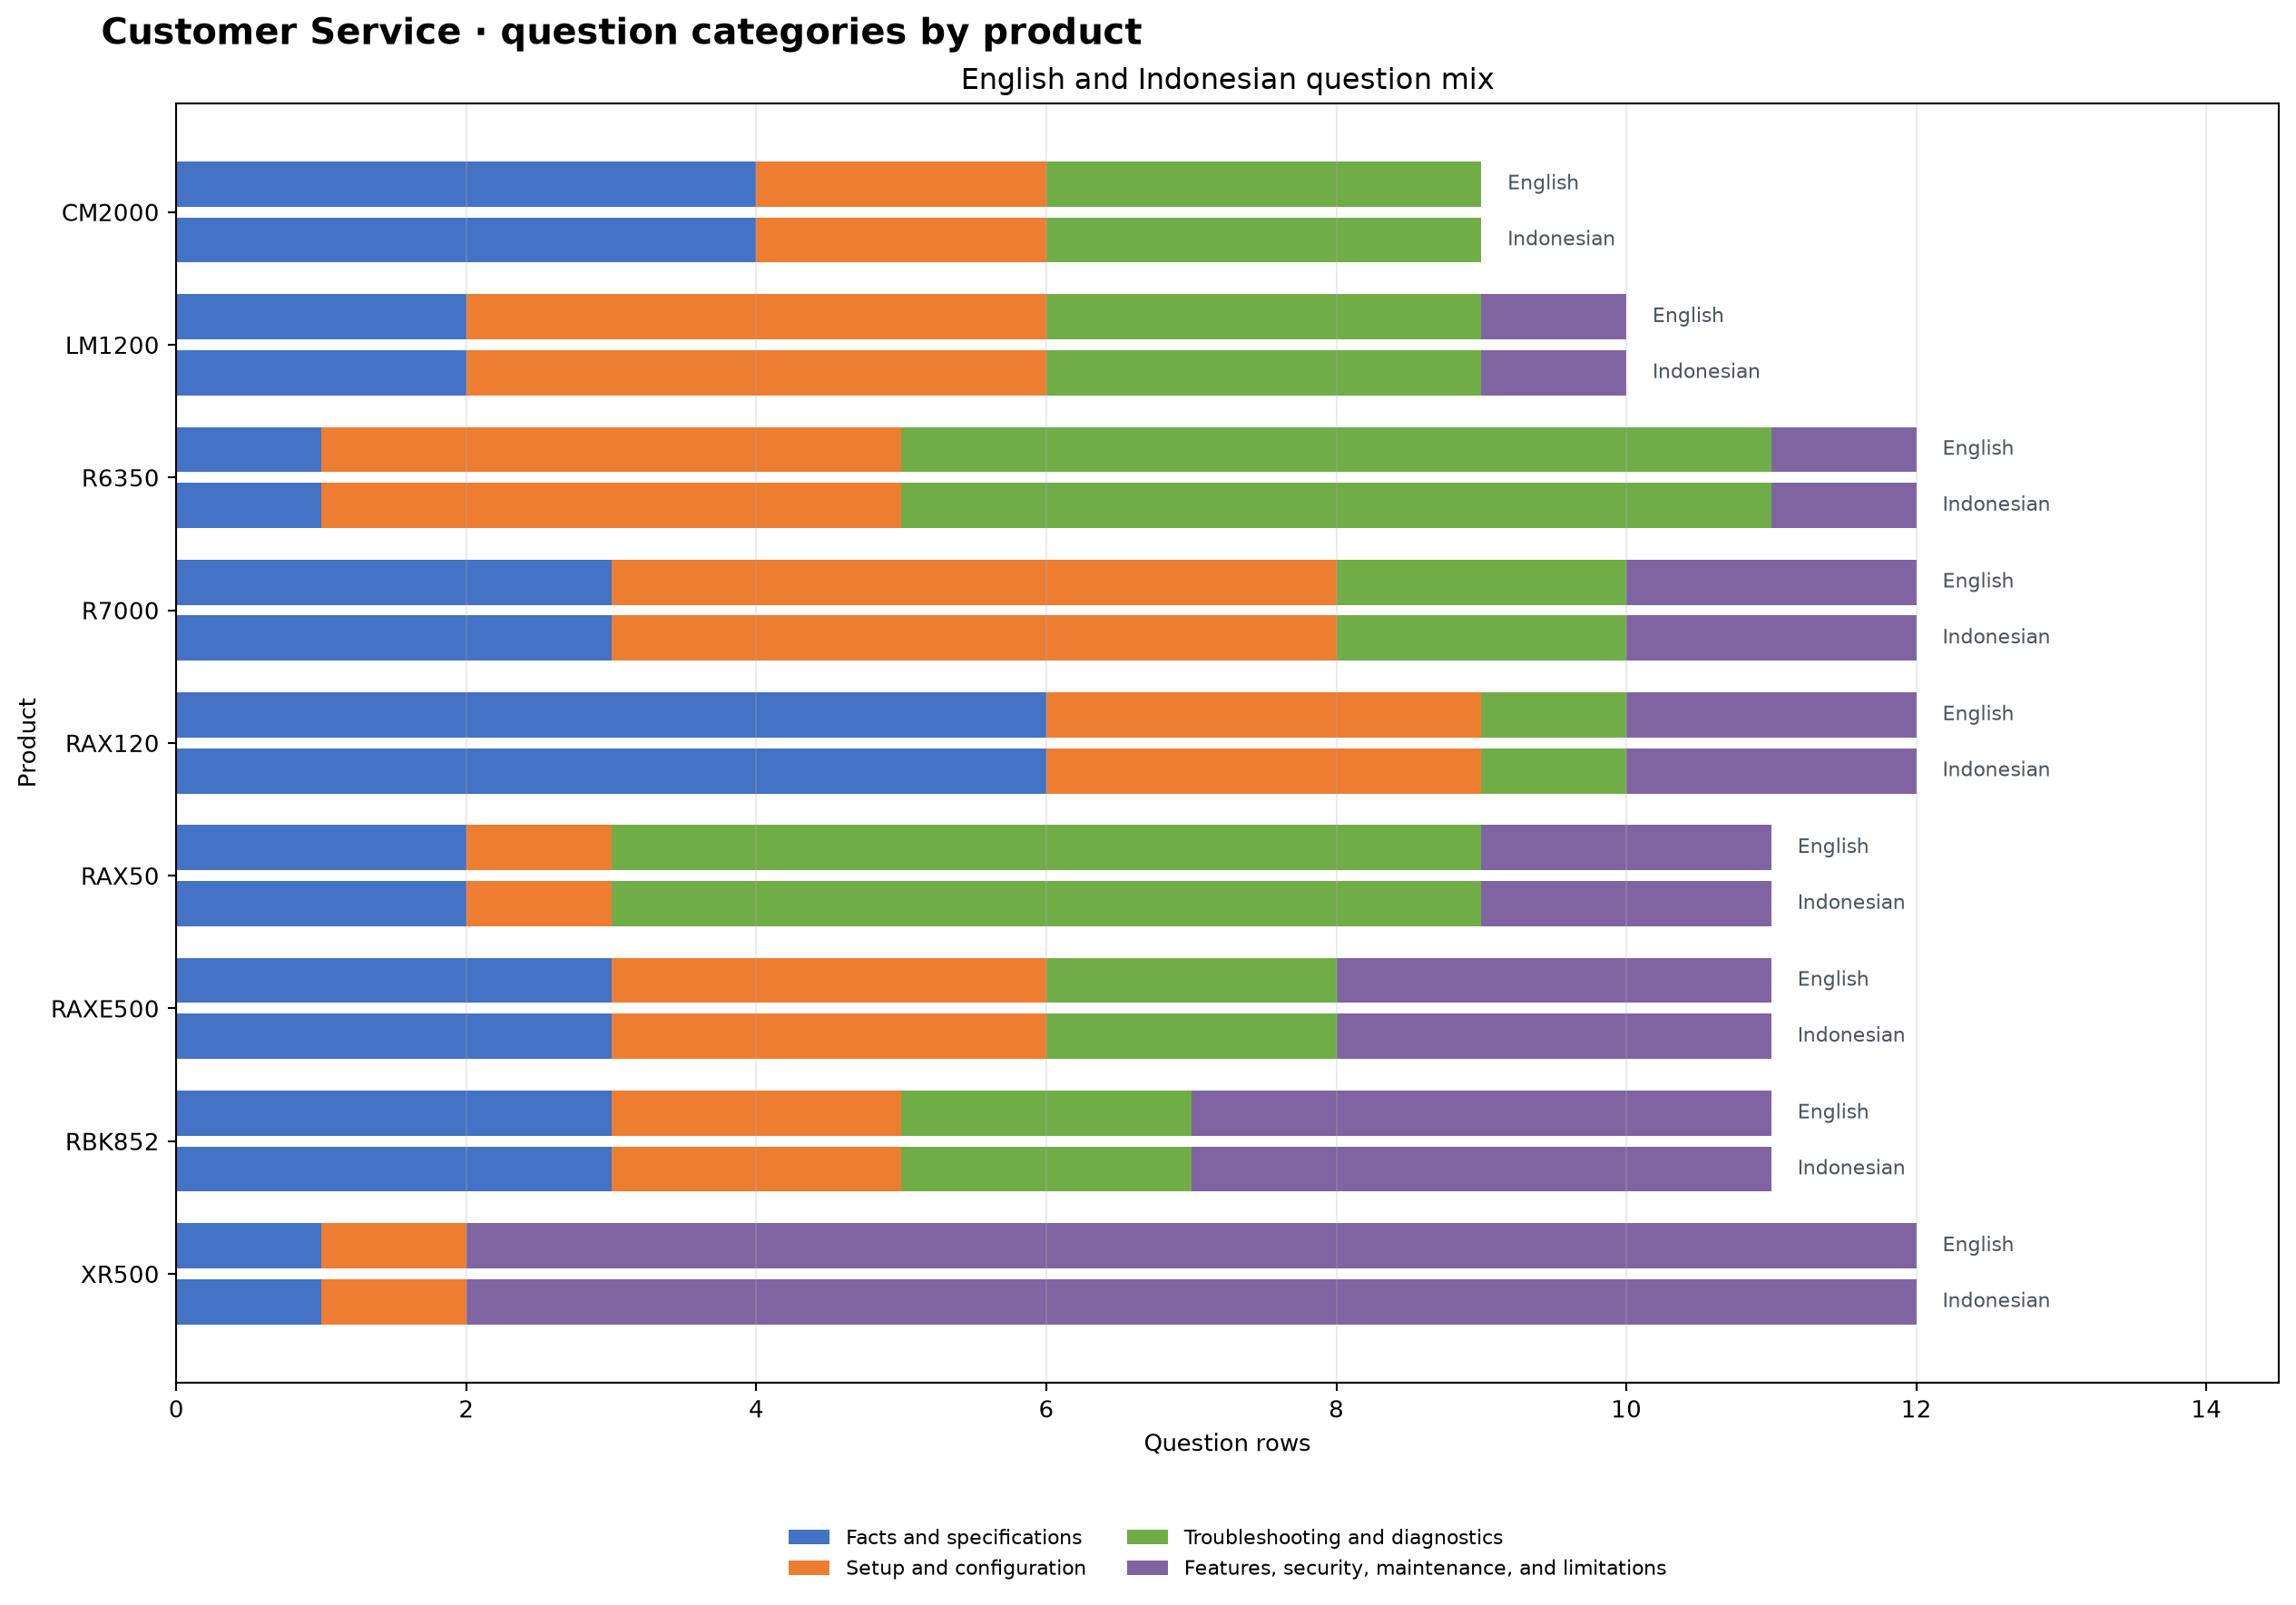
\includegraphics[width=\textwidth,height=0.62\textheight,keepaspectratio]{images/experiments/customer_service_revision/final_eda/question-category-distribution.png}
\caption{Komposisi kategori pertanyaan menurut produk dan bahasa}
\label{fig:customer-question-category-distribution}
\end{figure}

Gambar~\ref{fig:customer-question-page-distribution} menunjukkan bahwa konteks tersebar
di lima kelompok persentil posisi halaman relatif (P1 sampai P5) pada seluruh \emph{manual}.
Huruf P menunjukkan persentil, sedangkan angka setelahnya menunjukkan kelompok posisi
di dalam dokumen. P1 mencakup 0--20\% pertama dari panjang dokumen, P2 mencakup
20--40\%, P3 mencakup 40--60\%, P4 mencakup 60--80\%, dan P5 mencakup 80--100\%
terakhir. Posisi tersebut dihitung secara relatif terhadap jumlah halaman setiap dokumen.

\begin{figure}[H]
\centering
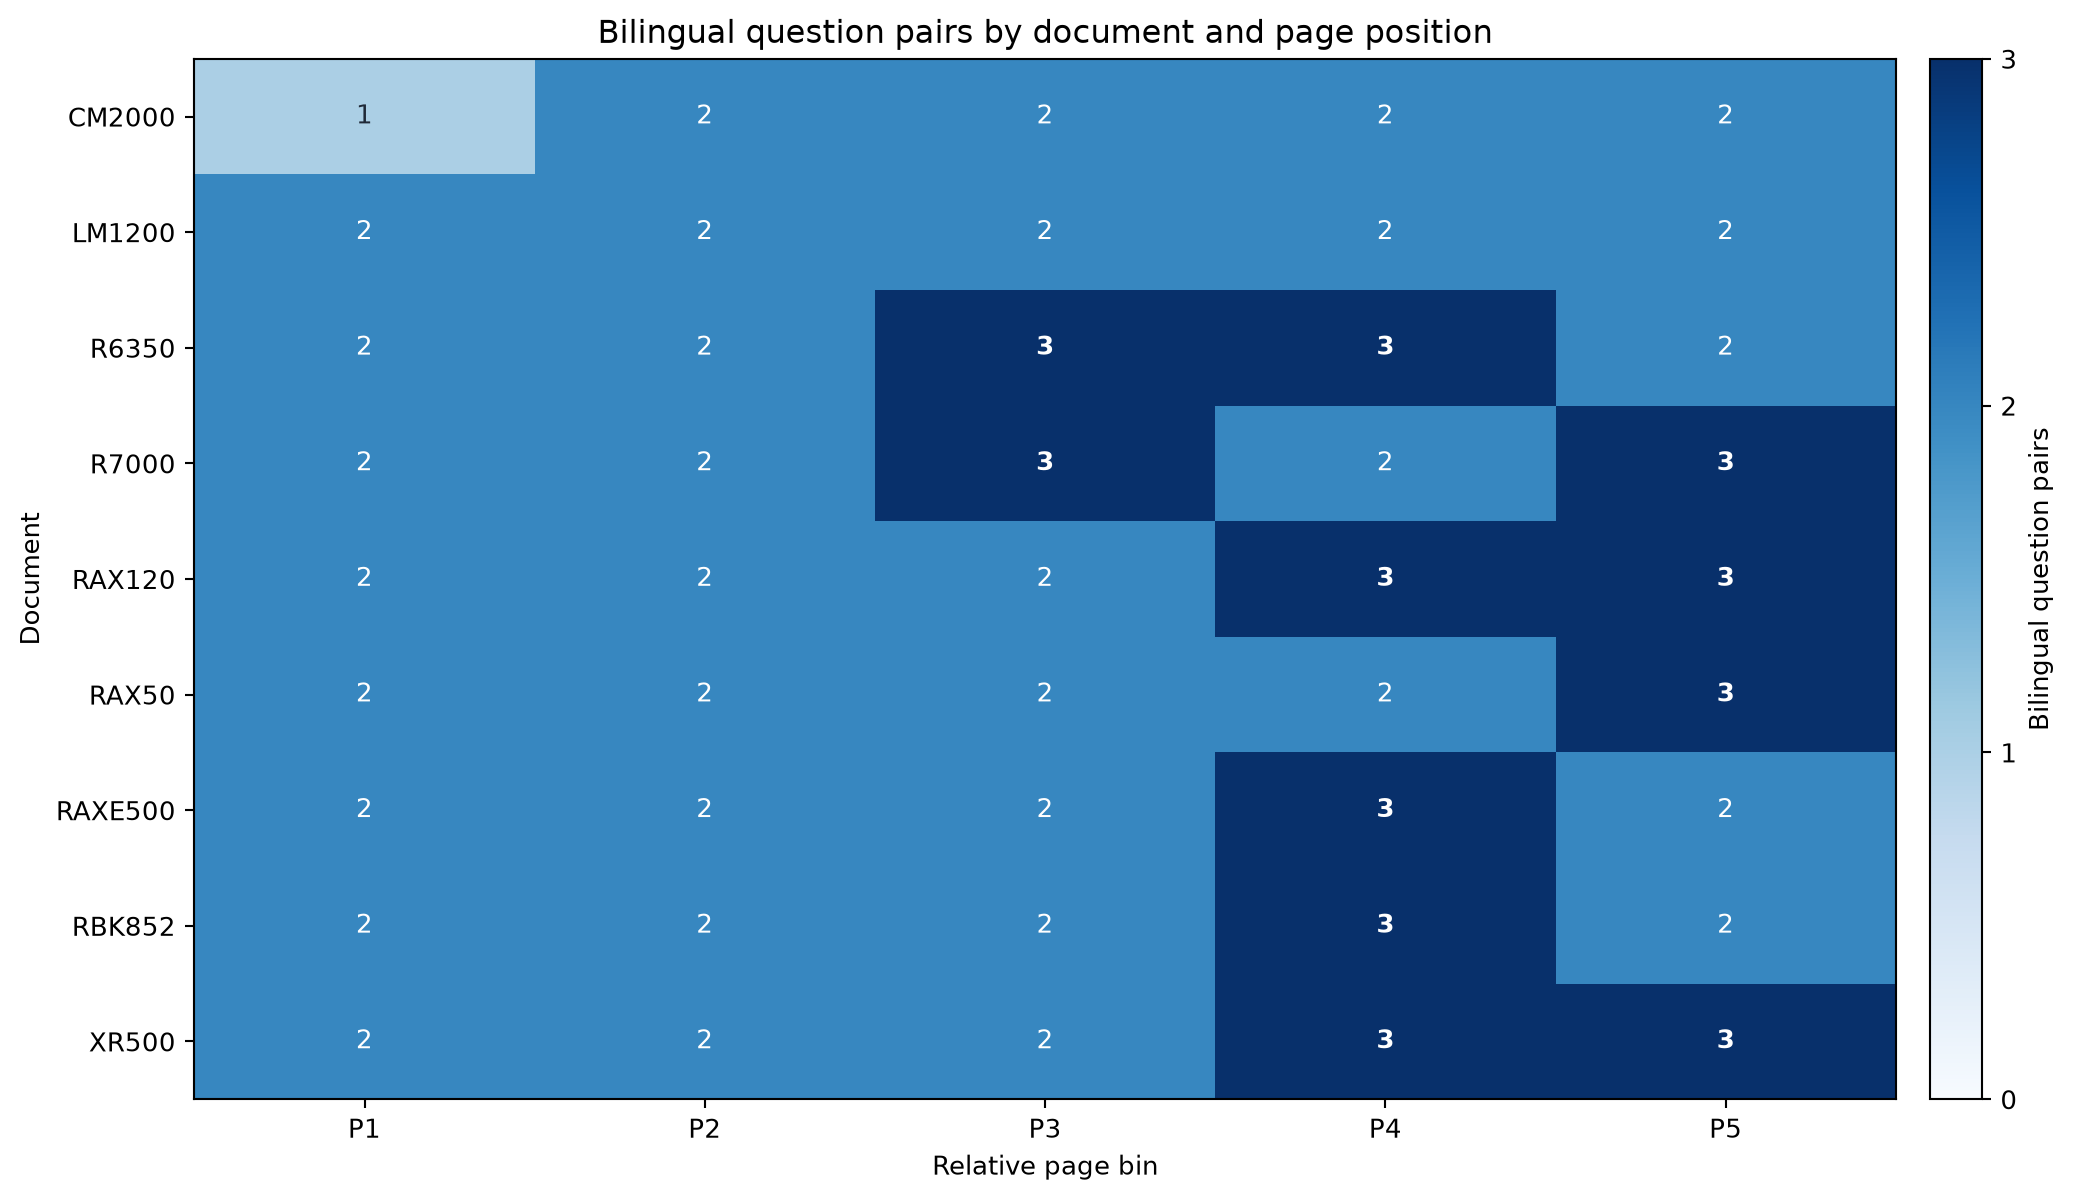
\includegraphics[width=\textwidth,height=0.55\textheight,keepaspectratio]{images/experiments/customer_service_revision/final_eda/question-page-distribution-by-document.png}
\caption{Sebaran pertanyaan menurut dokumen dan posisi halaman relatif}
\label{fig:customer-question-page-distribution}
\end{figure}

\emph{Heatmap} menunjukkan bahwa pertanyaan mencakup seluruh dokumen dan P1--P5, dengan
sedikit konsentrasi tambahan pada P4 dan P5 karena ketersediaan \emph{leaf outline}.

\subsection{Konfigurasi dan Metodologi Eksperimen}
\label{subsec:user-manual-config-method}

Pengukuran dibagi menjadi eksperimen \emph{retrieval} dan \emph{generation}. \emph{Retrieval} menilai konteks yang
dikembalikan, sedangkan \emph{generation} menilai jawaban yang dibentuk dari konteks tersebut. Lima
konfigurasi dan 200 pertanyaan yang sama digunakan pada kedua eksperimen. \emph{Reranker} dan
\emph{knowledge graph} dimatikan, sementara pembentukan jawaban hanya diaktifkan pada \emph{generation}.
\emph{Cutoff} \emph{retrieval} utama divariasikan dari \(K = 5\) sampai \(K = 60\). Titik \(K = 1\) dihitung
sebagai diagnosis top-1 terpisah untuk melihat seberapa sering kandidat pertama sudah memuat
\emph{context reference}. \emph{Parser}, \emph{dataset}, dan \emph{embedding} dipertahankan sama agar perubahan dapat
dikaitkan dengan \emph{chunker} atau \emph{indexer}.

Manual sumber berbahasa Inggris. Pertanyaan Inggris menguji pencarian satu bahasa dan pertanyaan
Indonesia menguji pencarian lintas bahasa. Keduanya dihitung dengan bobot yang sama.

Rincian konfigurasi, \emph{chunker}, dan \emph{indexer} yang dibandingkan disajikan pada
Tabel~\ref{tab:customer-config}.

\begin{table}[H]
\centering
\scriptsize
\caption{Konfigurasi eksperimen \emph{User Manual}}
\label{tab:customer-config}
\begin{tabularx}{\textwidth}{@{}>{\RaggedRight\arraybackslash}p{3.0cm}>{\RaggedRight\arraybackslash}p{5.0cm}>{\RaggedRight\arraybackslash}X@{}}
\toprule
\textbf{Konfigurasi} & \textbf{\emph{Chunker}} & \textbf{\emph{Indexer}}\\
\midrule
\emph{Structure-aware hybrid} & \texttt{generic-structure-aware}, \emph{target} \texttt{text\_block}, \emph{parent context}, 512 karakter & \texttt{hybrid-semantic-keyword}, \emph{dense} \texttt{BAAI/bge-m3} dan \emph{lexical}\\
Generik \emph{recursive} & \texttt{generic-recursive}, 512 karakter, \emph{overlap} 51 karakter & \texttt{hybrid-semantic-keyword}, \emph{dense} dan \emph{lexical}\\
\emph{Baseline chunker: Sliding-window} & \texttt{generic-sliding-window}, jendela 512 karakter, \emph{overlap} 51 karakter & \texttt{hybrid-semantic-keyword}, \emph{dense} dan \emph{lexical}\\
\emph{Structure-aware sparse} & \texttt{generic-structure-aware}, \emph{target} \texttt{text\_block}, \emph{parent context}, 512 karakter & \texttt{sparse-keyword}, \emph{lexical}\\
\emph{Structure-aware dense} & \texttt{generic-structure-aware}, \emph{target} \texttt{text\_block}, \emph{parent context}, 512 karakter & \texttt{dense-semantic}, \emph{dense} \texttt{BAAI/bge-m3}\\
\bottomrule
\end{tabularx}
\end{table}

Empat metrik berikut mengukur daftar \emph{context reference} dari setiap konfigurasi.
Untuk satu pertanyaan, \(R_K\) adalah hasil sampai peringkat \(K\), sedangkan \(G\) adalah
seluruh \emph{context reference} acuan. Setiap konfigurasi dihitung secara terpisah.

\noindent\textbf{\emph{Recall}@\(K\).}\quad
\emph{Recall} merupakan metrik utama untuk mengukur kelengkapan hasil:
\[
\mathrm{Recall}@K=\frac{\lvert R_K\cap G\rvert}{\lvert G\rvert}.
\]
Nilai dirata-ratakan atas seluruh pertanyaan. Nilai lebih tinggi menunjukkan lebih banyak
acuan ditemukan, tetapi tidak menunjukkan posisinya dalam daftar.

\noindent\textbf{\emph{Precision}@\(K\).}\quad
\emph{Precision} mengukur kepadatan acuan pada daftar hasil:
\[
\mathrm{Precision}@K=\frac{\lvert R_K\cap G\rvert}{K}.
\]
Nilai tinggi berarti lebih banyak kandidat yang relevan. Metrik ini menjadi pendukung karena
umumnya menurun ketika \(K\) diperbesar tanpa penambahan acuan yang sebanding.

\noindent\textbf{\emph{Mean Reciprocal Rank} (\emph{MRR}).}\quad
\emph{MRR} mengukur posisi \emph{reference} relevan pertama. Jika posisinya \(r\), reciprocal rank-nya
adalah \(1/r\), dan bernilai nol jika tidak ditemukan sampai \(K\). \emph{MRR} adalah rata-rata
\emph{reciprocal rank} seluruh pertanyaan. Nilai lebih tinggi berarti acuan pertama muncul lebih awal.

\noindent\textbf{\emph{Normalized Discounted Cumulative Gain} (\emph{NDCG}).}\quad
\emph{NDCG} menilai kualitas urutan berdasarkan relevansi bertingkat. \emph{Framework} \emph{Ragas}
menggunakan \texttt{openai/gpt-5.6-luna} dengan \emph{reasoning effort} \texttt{high}, dengan \emph{label}
0 untuk tidak mendukung, 1 untuk dukungan sebagian, dan 2 untuk dukungan langsung. Nilainya
dihitung sebagai
\[
\mathrm{DCG}@K=\sum_{i=1}^{K}\frac{2^{\mathrm{rel}_i}-1}{\log_2(i+1)},
\]
\[
\mathrm{NDCG}@K=\frac{\mathrm{DCG}@K}{\mathrm{IDCG}@K}.
\]
Nilai tinggi berarti konteks yang lebih membantu berada lebih awal. \emph{NDCG} melengkapi \emph{recall}
dan \emph{precision} dengan menilai urutan, bukan jumlah acuan yang ditemukan.

Dua metrik \emph{generation} dihitung terpisah untuk setiap konfigurasi menggunakan konteks
\(K = 10\), \emph{framework} \emph{Ragas}, dan \texttt{openai/gpt-5.6-luna}.

\noindent\textbf{\emph{Correctness}.}\quad
\emph{Correctness} adalah metrik utama \emph{generation} yang membandingkan jawaban dengan jawaban acuan.
Nilai tinggi menunjukkan jawaban tepat dan lengkap terhadap pertanyaan.

\noindent\textbf{\emph{Faithfulness}.}\quad
\emph{Faithfulness} memeriksa apakah klaim jawaban didukung oleh konteks yang diberikan. Nilai tinggi
menunjukkan jawaban tidak menambahkan informasi tanpa dasar.

\subsection{Eksperimen Per Komponen}
\label{subsec:user-manual-experiment-components}

\subsubsection{Strategi \emph{Chunking}}
\label{subsubsec:user-manual-chunking}

Perbandingan \emph{chunker} memakai \emph{hybrid indexer}, \emph{dataset}, \emph{parser}, dan \emph{model}
\emph{embedding} yang sama. Dengan cara ini, yang berubah hanya cara konteks sumber dibentuk sebelum
diindeks. \emph{Recall} kemudian menunjukkan seberapa lengkap setiap strategi segmentasi menjaga
\emph{context reference} tetap dapat ditemukan pada daftar teratas. \emph{Sliding-window} ditetapkan
sebagai \emph{baseline} \emph{chunker} karena merupakan pembagian jendela tetap dengan \emph{overlap} yang paling
sederhana. Konfigurasi \emph{structure-aware} adalah pendekatan yang diusulkan dan diuji terhadap
\emph{baseline} tersebut. Konfigurasi yang dibandingkan
diringkas pada Tabel~\ref{tab:customer-chunker-config}.

\begin{table}[H]
\centering
\scriptsize
\caption{Konfigurasi \emph{chunker} pada eksperimen \emph{User Manual}}
\label{tab:customer-chunker-config}
\begin{tabularx}{\textwidth}{@{}>{\RaggedRight\arraybackslash}p{3.1cm}>{\RaggedRight\arraybackslash}p{4.2cm}>{\RaggedRight\arraybackslash}X@{}}
\toprule
\textbf{Strategi} & \textbf{\emph{Plugin}} & \textbf{Konfigurasi utama}\\
\midrule
\emph{Structure-aware hybrid} & \texttt{generic-structure-aware} & \emph{Target} \texttt{text\_block}, \emph{parent context}, maksimum 512 karakter\\
\emph{Recursive} & \texttt{generic-recursive} & Maksimum 512 karakter, \emph{overlap} 51 karakter, \emph{separator} bertingkat\\
\emph{Baseline chunker: Sliding-window} & \texttt{generic-sliding-window} & Jendela 512 karakter dan \emph{overlap} 51 karakter\\
\bottomrule
\end{tabularx}
\end{table}

\begin{figure}[H]
\centering
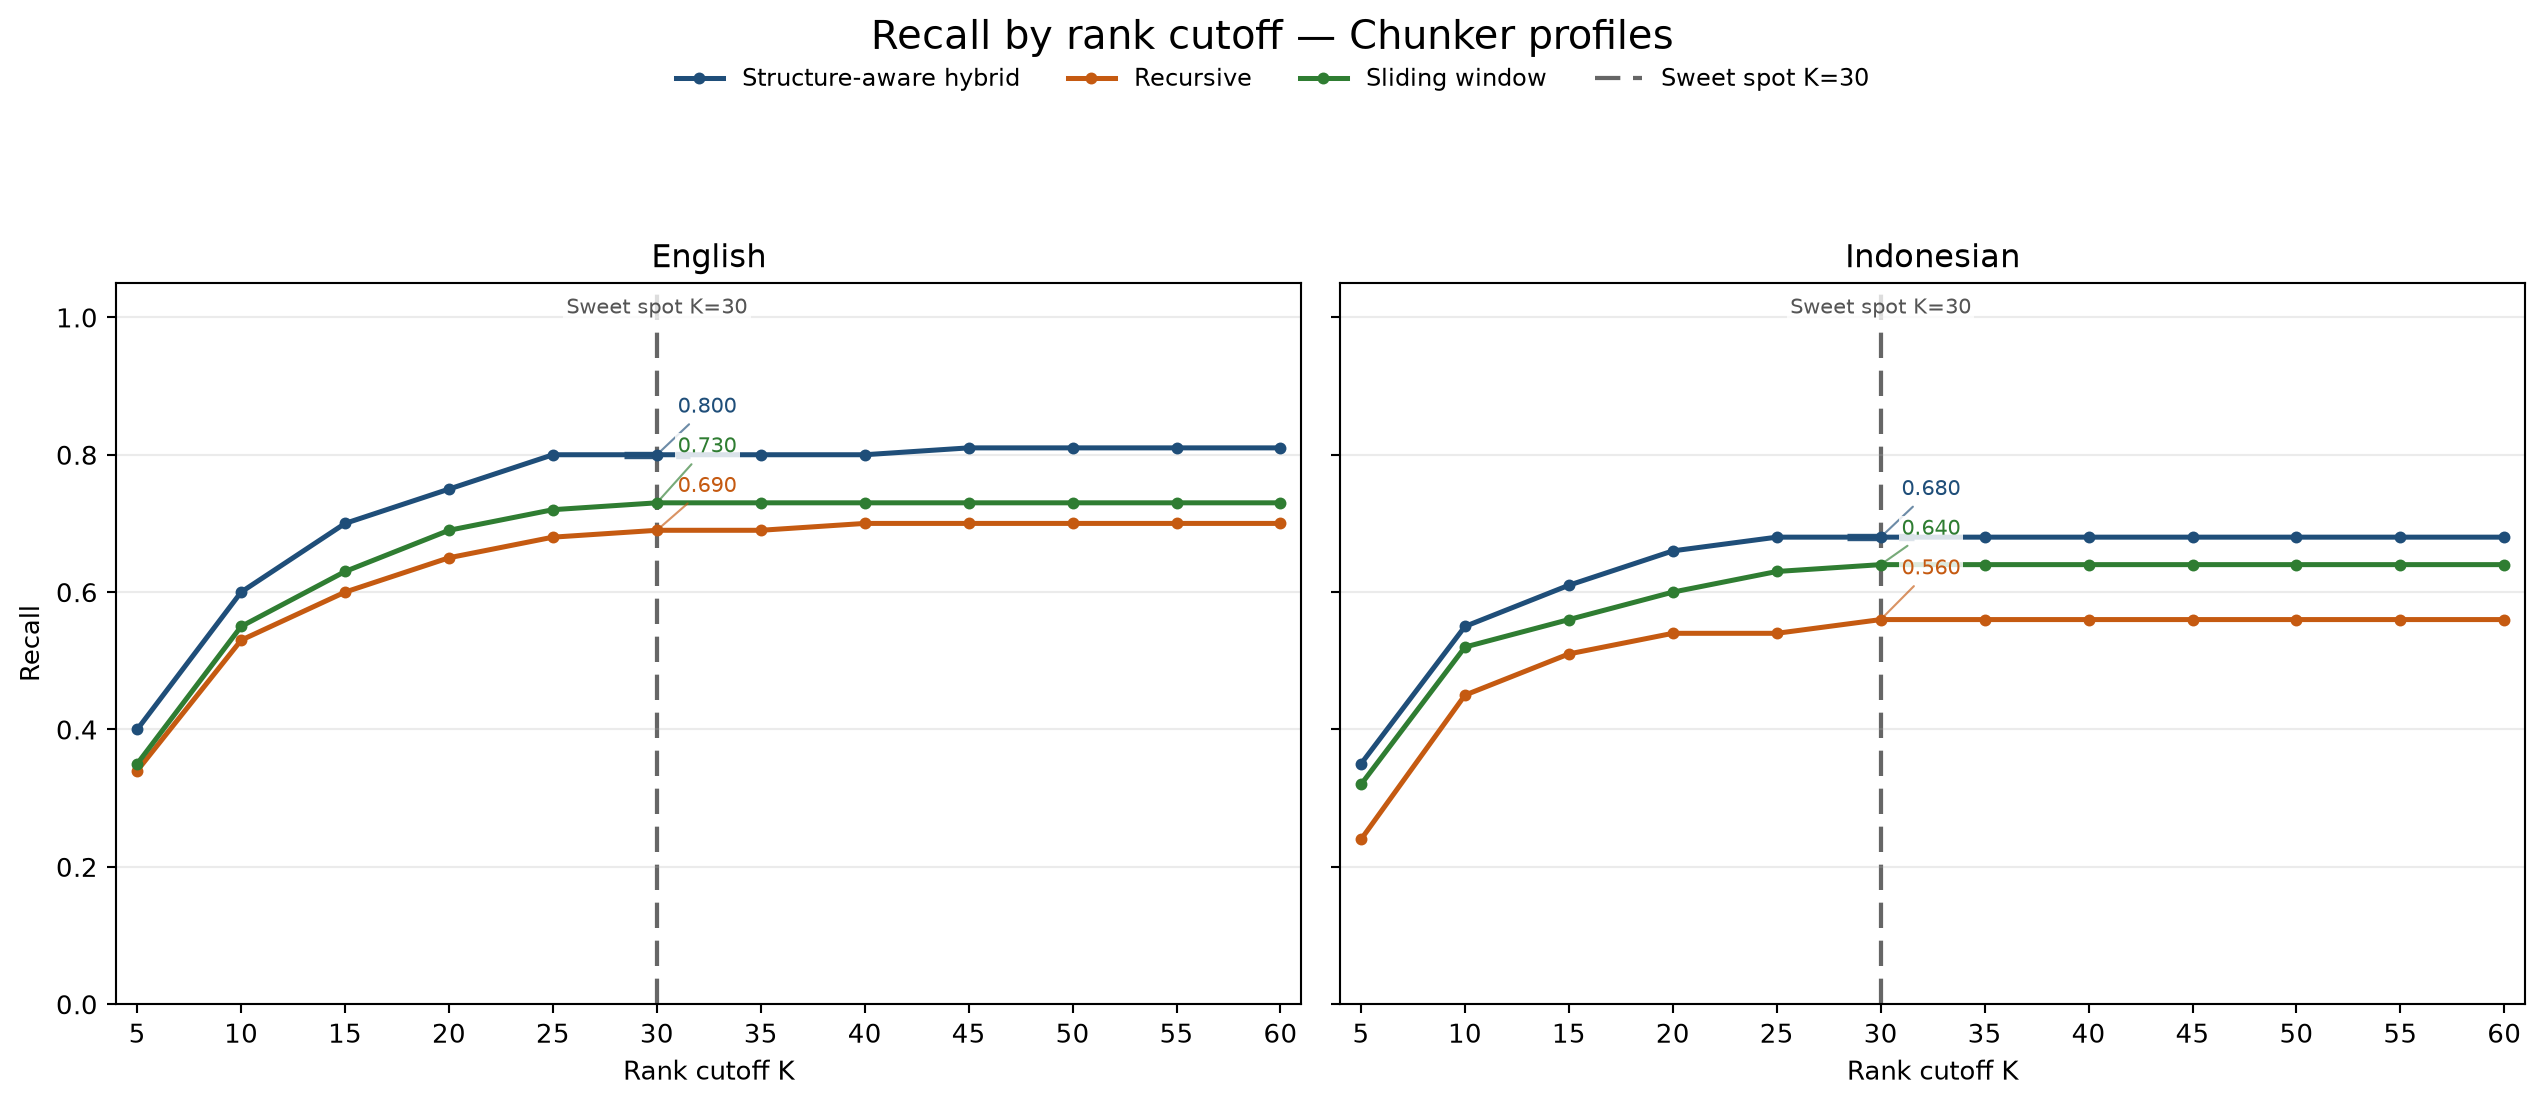
\includegraphics[width=\textwidth,height=0.52\textheight,keepaspectratio]{images/experiments/customer_service_revision/final_eda/recall-chunker.png}
\caption{Kurva \emph{context reference} \emph{recall} menurut \emph{cutoff} untuk konfigurasi \emph{chunker}}
\label{fig:customer-chunker-recall}
\end{figure}

Pada Gambar~\ref{fig:customer-chunker-recall}, ketiga kurva meningkat ketika kandidat
ditambah dari \(K = 5\) sampai sekitar \(K = 20\). Pada tahap ini, kandidat baru masih sering
membawa \emph{context reference} yang belum ditemukan. Setelah itu kenaikannya melambat. Pada
\(K = 30\), \emph{recall} gabungan mencapai 0,740 untuk \emph{Structure-aware hybrid}, 0,685 untuk
\emph{Sliding-window}, dan 0,625 untuk \emph{Recursive}. Nilai \emph{Structure-aware hybrid}
bahkan sudah 0,740 pada \(K = 25\), sehingga selisihnya dari \(K = 25\) ke \(K = 30\) adalah
0,000. Selisih pada \emph{Sliding-window} hanya 0,010 dan pada \emph{Recursive} 0,015.
Ketika \emph{cutoff} diperbesar lagi hingga \(K = 60\), nilainya hanya berubah menjadi 0,745,
0,685, dan 0,630. Artinya, sebagian besar \emph{reference} yang mudah ditemukan sudah masuk sebelum
\(K = 30\), sedangkan kandidat setelahnya lebih banyak berada pada ekor \emph{ranking}. Karena itu,
\(K = 30\) dipakai sebagai \emph{sweet spot} bersama.

Dengan \emph{Sliding-window} sebagai \emph{baseline}, \emph{Structure-aware} \emph{hybrid} meningkatkan \emph{recall} dari
0,685 menjadi 0,740, atau delta +0,055 pada \(K = 30\). Hasil ini menunjukkan bahwa strategi
\emph{structure-aware} yang diusulkan mengalahkan pendekatan segmentasi naif pada metrik utama.

Perbedaan ini juga konsisten pada kedua bahasa. Pada \(K = 30\), \emph{recall} bahasa Inggris dan
Indonesia untuk \emph{Structure-aware hybrid} adalah 0,800 dan 0,680. Untuk
\emph{Sliding-window} nilainya 0,730 dan 0,640, sedangkan \emph{Recursive} memperoleh 0,690
dan 0,560. Bahasa Inggris lebih tinggi karena istilah pada pertanyaan sama dengan bahasa
manual, tetapi urutan strategi tidak berubah. Dengan demikian, keunggulan \emph{structure-aware}
bukan hanya berasal dari salah satu bahasa.

\begin{figure}[H]
\centering
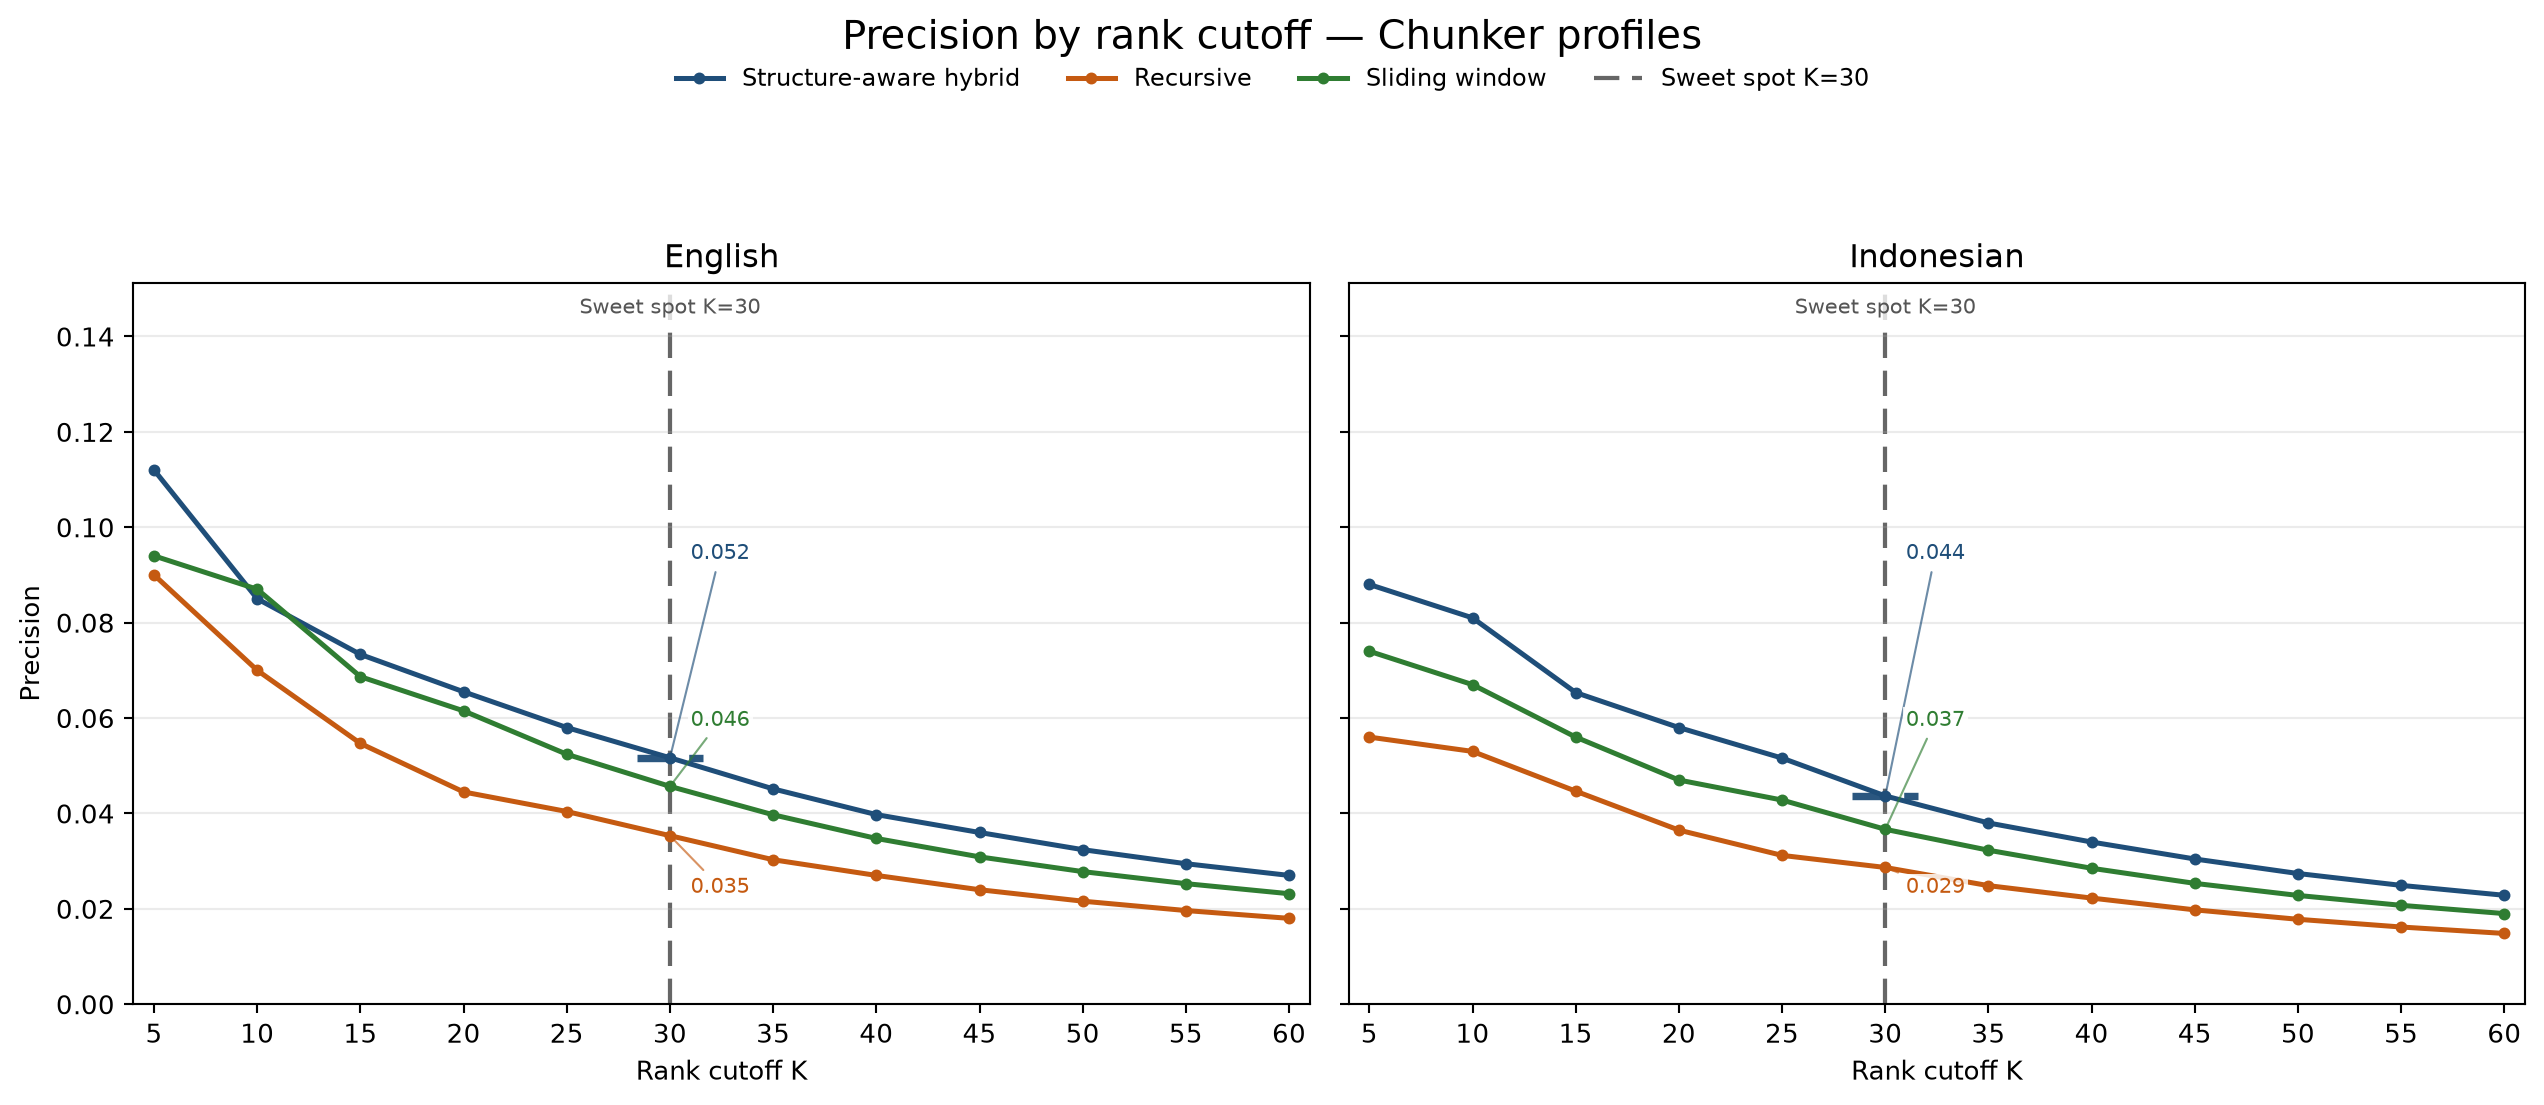
\includegraphics[width=\textwidth,height=0.52\textheight,keepaspectratio]{images/experiments/customer_service_revision/final_eda/precision-chunker.png}
\caption{Kurva \emph{context reference} \emph{precision} menurut \emph{cutoff} untuk konfigurasi \emph{chunker}}
\label{fig:customer-chunker-precision}
\end{figure}

Pada Gambar~\ref{fig:customer-chunker-precision}, \emph{precision} turun ketika \emph{cutoff} bertambah
karena penyebutnya adalah seluruh kandidat yang dikembalikan, sedangkan jumlah context
\emph{reference} baru tidak bertambah dengan laju yang sama. Pada \(K = 10\), nilainya 0,083 untuk
\emph{Structure-aware hybrid}, 0,077 untuk \emph{Sliding-window}, dan 0,062 untuk
\emph{Recursive}. Pada \(K = 30\), nilainya menjadi 0,048, 0,041, dan 0,032, lalu turun lagi
menjadi 0,025, 0,021, dan 0,016 pada \(K = 60\). Pola ini tidak berarti bahwa \emph{recall}
menurun. Pola ini menunjukkan bahwa kandidat tambahan semakin banyak berisi konteks yang
tidak menambah \emph{reference} baru. \emph{Structure-aware} tetap memiliki \emph{precision} tertinggi karena
segmentasinya lebih sering mengirimkan unit konteks yang memang memuat \emph{reference}.

\begin{figure}[H]
\centering
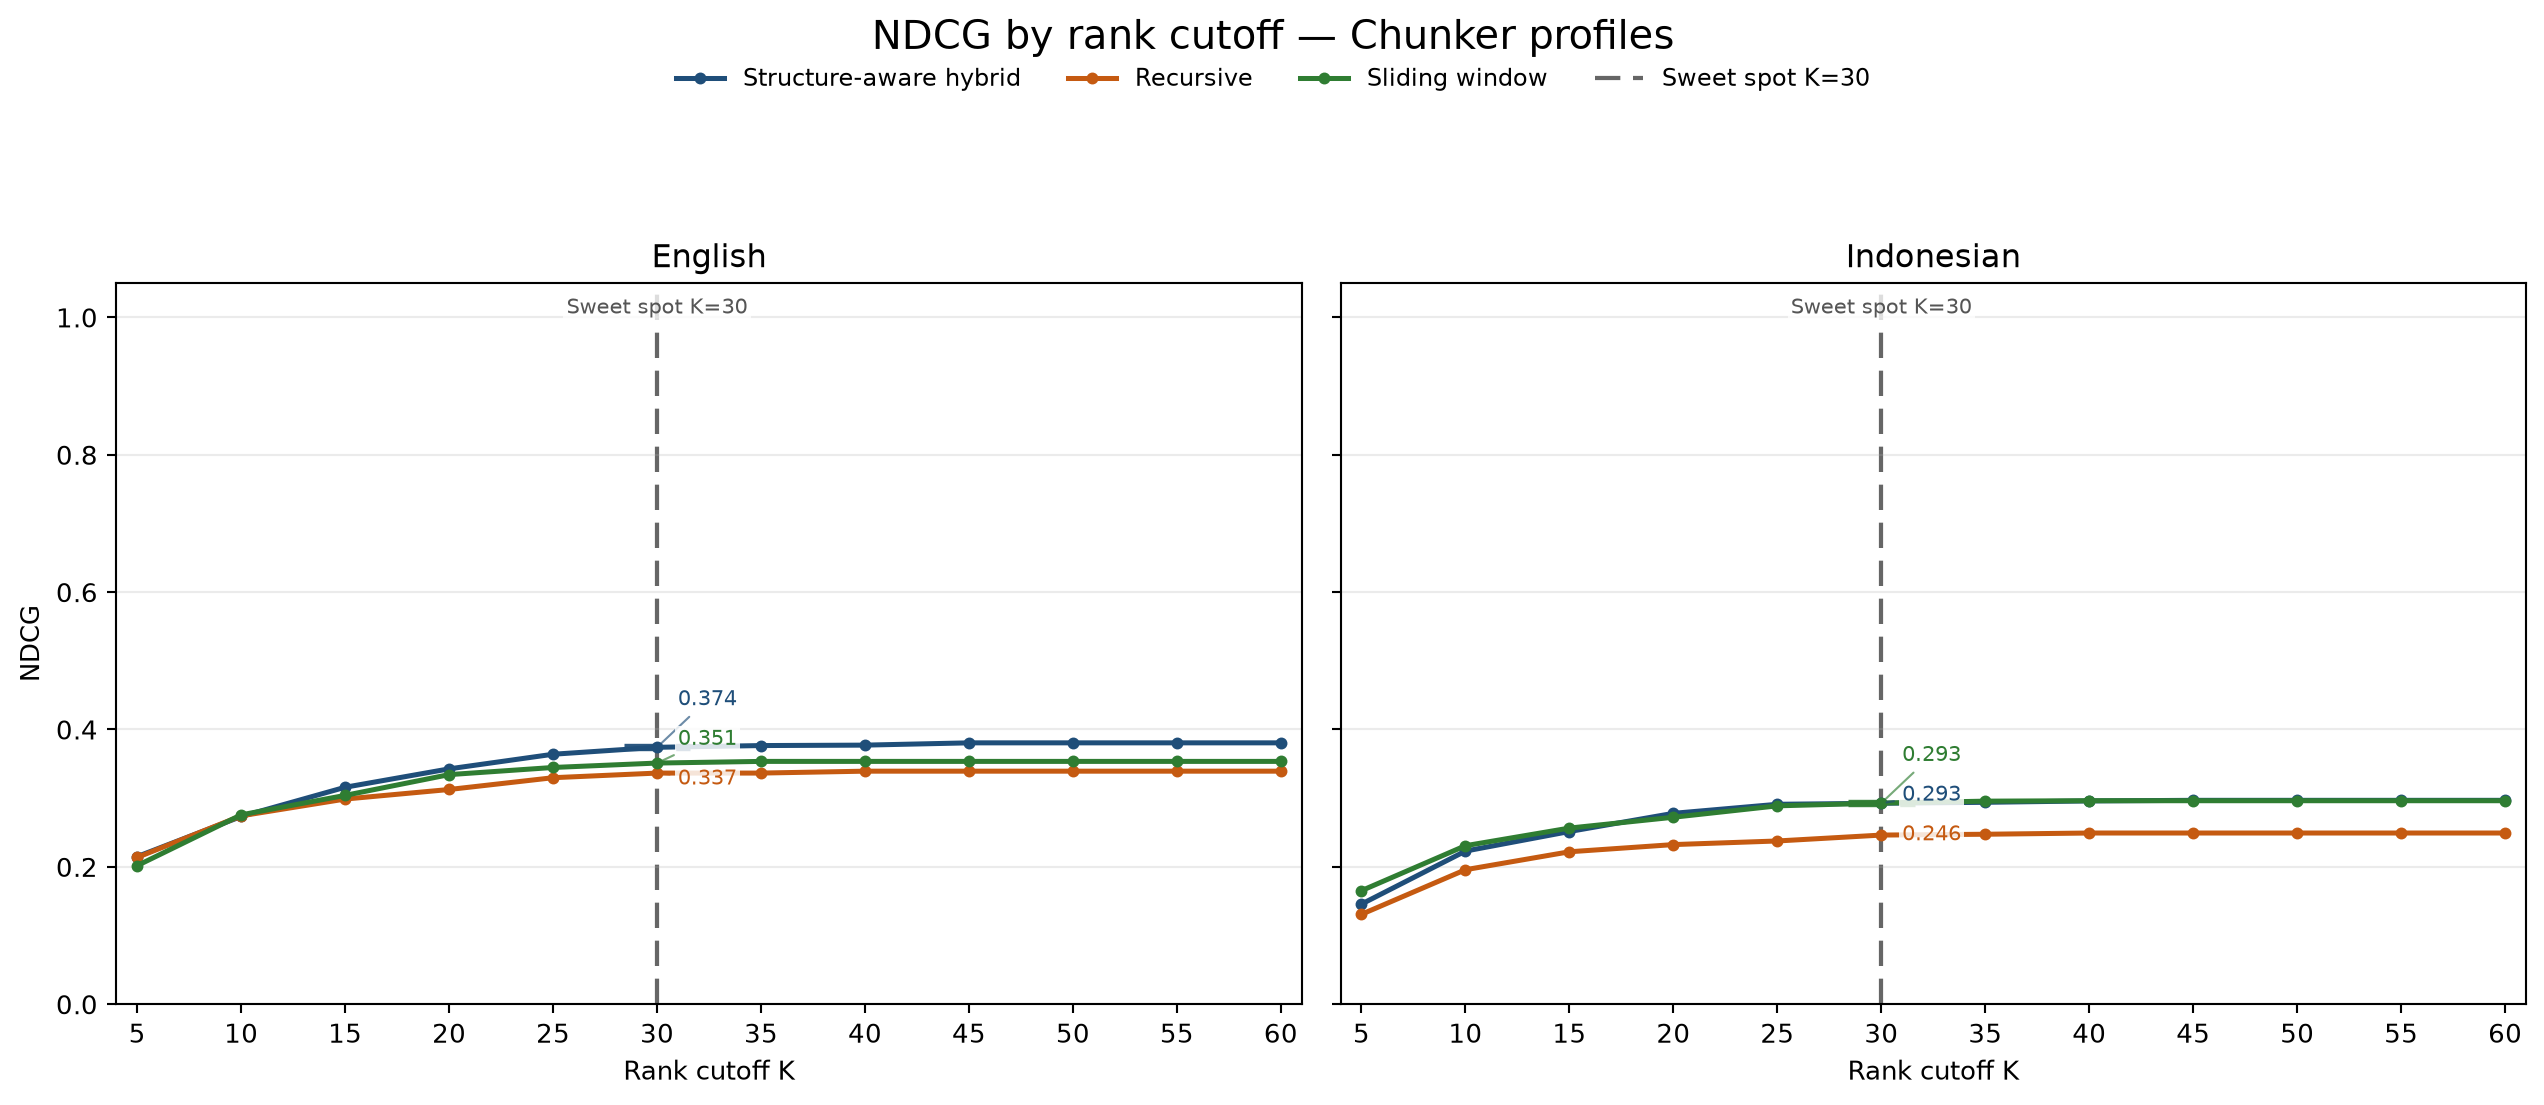
\includegraphics[width=\textwidth,height=0.52\textheight,keepaspectratio]{images/experiments/customer_service_revision/final_eda/ndcg-chunker.png}
\caption{Kurva \emph{NDCG} menurut \emph{cutoff} untuk konfigurasi \emph{chunker}}
\label{fig:customer-chunker-ndcg}
\end{figure}

Pada Gambar~\ref{fig:customer-chunker-ndcg}, \emph{NDCG} pada \(K = 30\) adalah 0,333 untuk
\emph{Structure-aware hybrid}, 0,322 untuk \emph{Sliding-window}, dan 0,291 untuk
\emph{Recursive}. Nilai tersebut menunjukkan bahwa \emph{reference} pada \emph{structure-aware} lebih
sering muncul di bagian awal \emph{ranking}. Pada \(K = 60\), nilainya hanya berubah menjadi 0,339,
0,325, dan 0,294. Jadi penambahan \emph{cutoff} setelah \(K = 30\) tidak banyak memperbaiki posisi
\emph{reference}, walaupun masih dapat menambah sedikit cakupan \emph{recall}.

\begin{figure}[H]
\centering
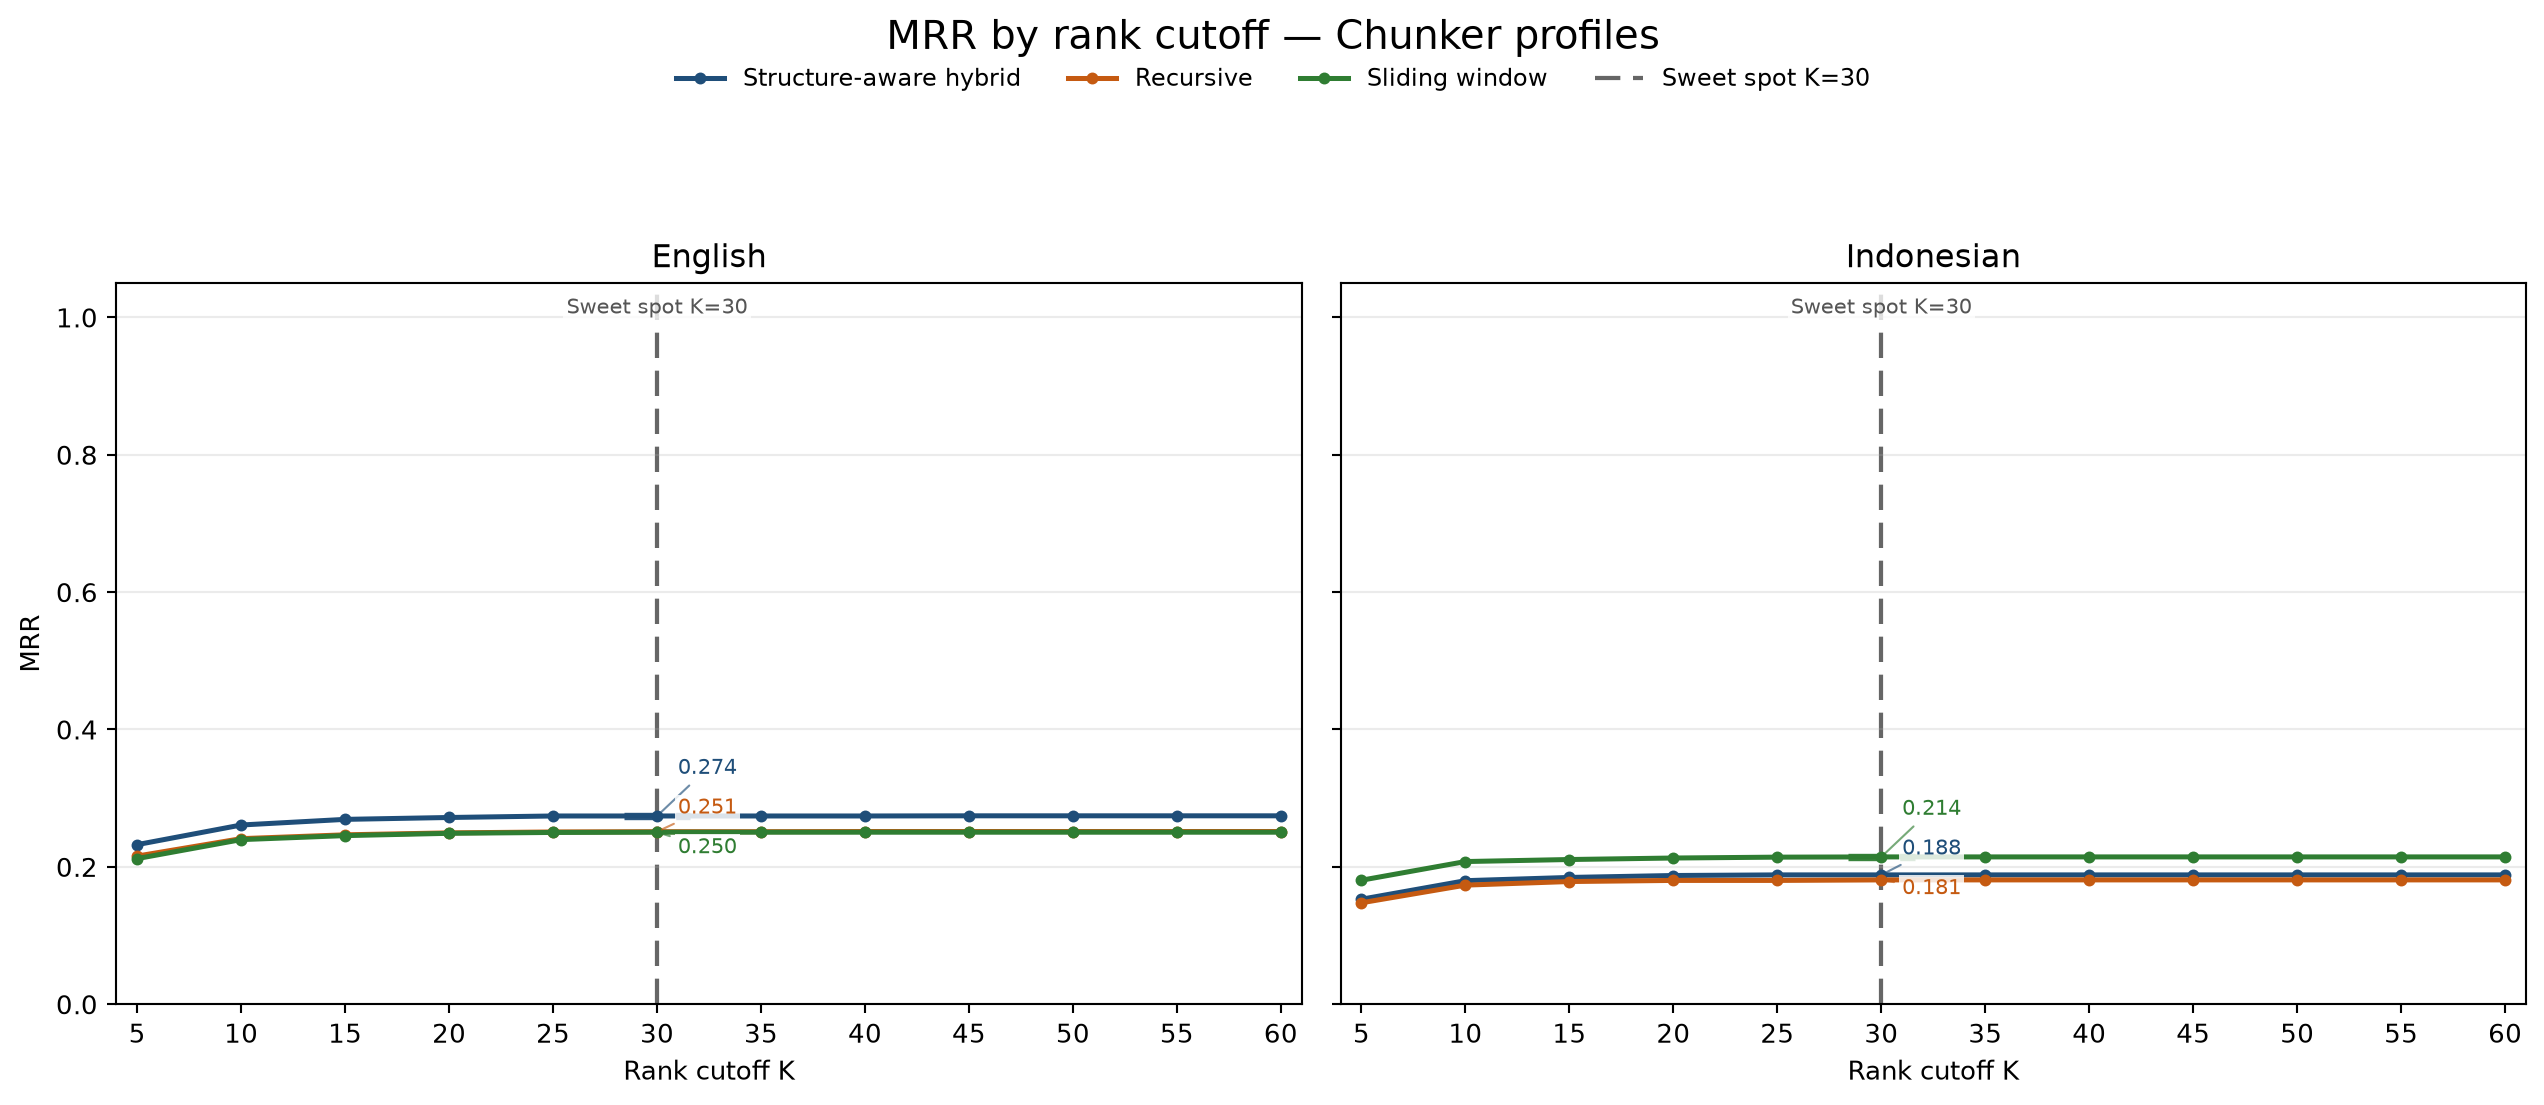
\includegraphics[width=\textwidth,height=0.52\textheight,keepaspectratio]{images/experiments/customer_service_revision/final_eda/mrr-chunker.png}
\caption{Kurva \emph{MRR} menurut \emph{cutoff} untuk konfigurasi \emph{chunker}}
\label{fig:customer-chunker-mrr}
\end{figure}

Pada Gambar~\ref{fig:customer-chunker-mrr}, \emph{MRR} pada \(K = 30\) adalah 0,232 untuk
\emph{Sliding-window}, 0,231 untuk \emph{Structure-aware hybrid}, dan 0,216 untuk
\emph{Recursive}. Nilai \emph{Sliding-window} yang sedikit lebih tinggi tidak berarti bahwa
strategi ini menemukan lebih banyak \emph{reference}. \emph{MRR} hanya melihat posisi \emph{reference} pertama.
Satu \emph{reference} yang muncul sangat awal dapat menaikkan \emph{MRR}, walaupun \emph{reference} lain belum
terambil. Karena itu, hasil ini dapat dibaca sebagai keunggulan kecil pada posisi hit pertama,
sementara \emph{recall} tetap menunjukkan bahwa \emph{structure-aware} menemukan lebih banyak \emph{reference}
secara keseluruhan. Pada \(K = 60\), \emph{MRR} hampir tidak berubah menjadi 0,231, 0,232, dan 0,216.

\begin{figure}[H]
\centering
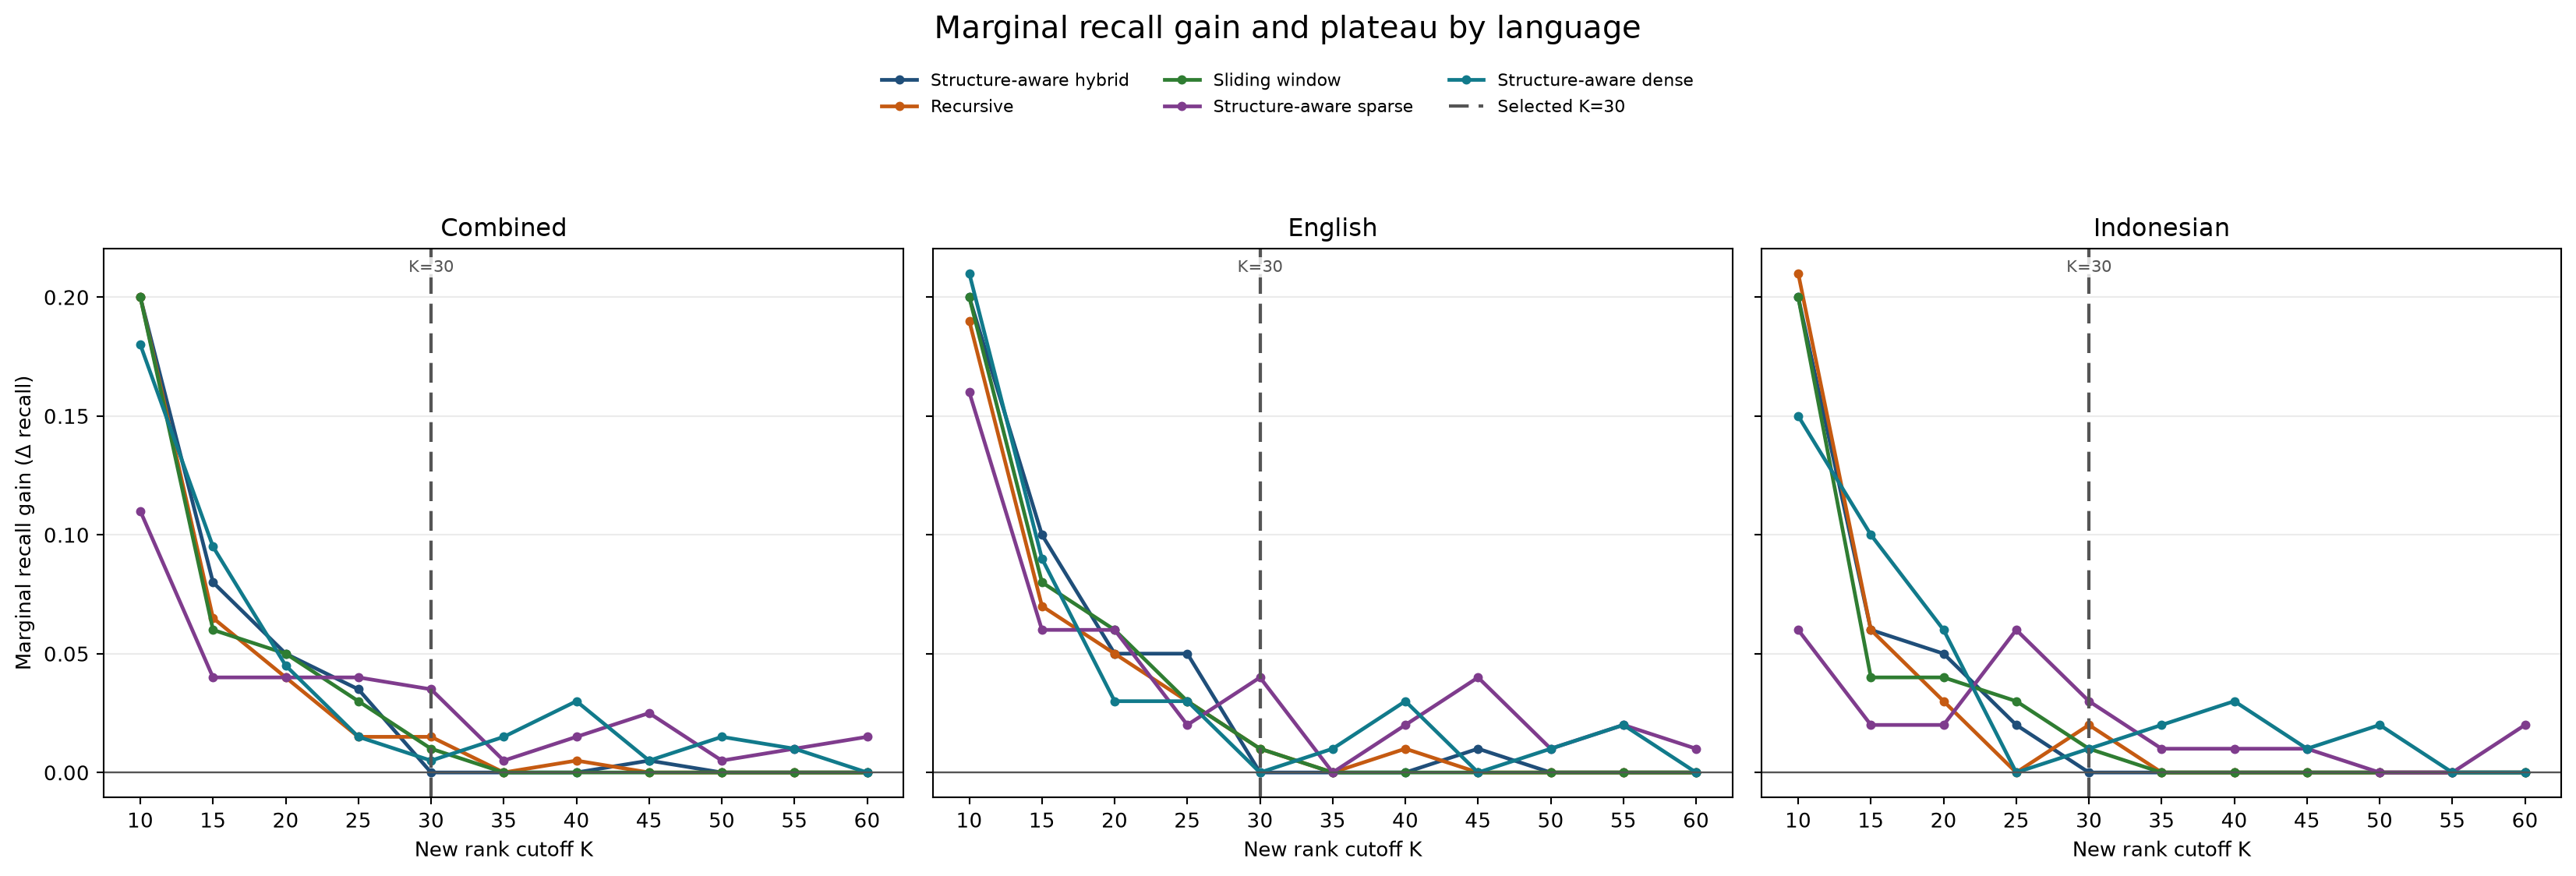
\includegraphics[width=\textwidth,height=0.43\textheight,keepaspectratio]{images/experiments/customer_service_revision/final_eda/recall-marginal-delta.png}
\caption{Selisih \emph{recall} per kenaikan K untuk gabungan, Inggris, dan Indonesia}
\label{fig:customer-recall-delta}
\end{figure}

Gambar~\ref{fig:customer-recall-delta} memperlihatkan bahwa tambahan \emph{recall} terbesar terjadi
pada kenaikan \emph{cutoff} awal. Di sekitar \(K = 25\) sampai \(K = 30\), tambahan tersebut sudah
mendekati nol. Setelah \(K = 30\), \emph{structure-aware} hanya bertambah 0,005 sampai \(K = 60\),
\emph{recursive} bertambah 0,005, dan \emph{sliding-window} tidak bertambah. Dengan demikian, \(K = 30\)
memberi cakupan yang hampir sama dengan \emph{cutoff} yang lebih besar tanpa membawa seluruh ekor
kandidat ke tahap \emph{downstream}.

\begin{table}[H]
\centering
\scriptsize
\caption{Hasil strategi \emph{chunking} pada \emph{sweet spot} masing-masing}
\label{tab:customer-chunking-results}
\begin{tabularx}{\textwidth}{@{}>{\RaggedRight\arraybackslash}p{3.7cm} r r r r r@{}}
\toprule
\textbf{Strategi} & \textbf{K} & \textbf{\emph{Recall}} & \textbf{\emph{Precision}} & \textbf{\emph{NDCG}} & \textbf{\emph{MRR}}\\
\midrule
\emph{Structure-aware hybrid} & 30 & \textbf{0,740} & \textbf{0,048} & \textbf{0,333} & 0,231\\
\emph{Recursive} \emph{chunker} & 30 & 0,625 & 0,032 & 0,291 & 0,216\\
\emph{Baseline chunker: Sliding-window} & 30 & 0,685 & 0,041 & 0,322 & \textbf{0,232}\\
\bottomrule
\end{tabularx}
\end{table}

Pada \(K = 30\), \emph{recall} \emph{Structure-aware hybrid}, \emph{Sliding-window}, dan
\emph{Recursive} adalah 0,740, 0,685, dan 0,625. Karena \emph{parser}, \emph{dataset}, \emph{embedding}, dan
\emph{indexer} sama, selisih ini menunjukkan dampak segmentasi, bukan perubahan pada sumber
pertanyaan atau mesin pencarian. \emph{Structure-aware hybrid} unggul pada seluruh kategori.
\emph{Recall} per kategori adalah 0,780, 0,720, 0,740, dan 0,720 untuk fakta dan spesifikasi,
penyiapan dan konfigurasi, diagnosis, serta fitur, keamanan, pemeliharaan, dan keterbatasan.
\emph{Sliding-window} memperoleh 0,700, 0,680, 0,660, dan 0,700, sedangkan
\emph{Recursive} memperoleh 0,700, 0,600, 0,560, dan 0,640. Selisih terbesar muncul pada
diagnosis dan penyiapan karena pertanyaan pada dua kategori tersebut lebih sering membutuhkan
beberapa informasi yang saling berkaitan, bukan satu istilah tunggal.

Berdasarkan hasil analisis, unit \emph{structure-aware} lebih sering mempertahankan isi
jawaban bersama petunjuk bagian manual yang menjelaskan fitur atau langkahnya. \emph{Sliding-window}
berada di posisi kedua karena \emph{overlap} menjaga teks yang berdekatan ketika \emph{reference} berada di
dekat batas segmen. Namun, \emph{overlap} juga dapat mengulang teks yang sama pada beberapa kandidat,
sehingga slot tambahan tidak selalu menghasilkan \emph{reference} baru. \emph{Recursive} paling rendah pada
penyiapan dan diagnosis karena informasi tindakan dan syaratnya lebih sering muncul pada
kandidat yang terpisah. Temuan ini menjelaskan mengapa \emph{sliding} masih kompetitif, tetapi belum
mencapai cakupan \emph{structure-aware}.

Metrik pendukung memperkuat pembacaan tersebut. \emph{Structure-aware} memiliki \emph{precision} 0,048 dan
\emph{NDCG} 0,333, \emph{sliding} 0,041 dan 0,322, serta \emph{recursive} 0,032 dan 0,291. \emph{MRR} \emph{sliding} 0,232
hanya sedikit di atas \emph{structure-aware} 0,231 karena hit pertamanya lebih awal pada sebagian
pertanyaan. Pada perbandingan bahasa pada \(K = 30\), \emph{Structure-aware hybrid} mencapai \emph{recall}
0,800 untuk pertanyaan Inggris dan 0,680 untuk pertanyaan Indonesia. Selisihnya adalah
0,120. \emph{Sliding-window} memperoleh 0,730 dan 0,640 dengan selisih 0,090, sedangkan
\emph{Recursive} memperoleh 0,690 dan 0,560 dengan selisih 0,130. Selisih positif menunjukkan bahwa
\emph{recall} turun ketika bahasa pertanyaan berbeda dari bahasa manual sumber. Manual sumber berbahasa
Inggris, sehingga pertanyaan Inggris memiliki kecocokan istilah yang lebih langsung. Pertanyaan
Indonesia memerlukan pemetaan lintas bahasa oleh \emph{embedding} \emph{multilingual}, dan istilah teknis atau
parafrasa tidak selalu memiliki kecocokan yang sama kuat. Meskipun tingkat \emph{recall} berubah, urutan
strategi tidak berubah: \emph{Structure-aware hybrid} tetap tertinggi, diikuti \emph{Sliding-window}
dan \emph{Recursive}. Konteks yang mempertahankan isi jawaban bersama petunjuk bagian dokumen
membantu \emph{Structure-aware hybrid} tetap unggul pada kedua bahasa. Karena \emph{recall} adalah metrik
utama, \emph{Structure-aware hybrid} dipilih untuk eksperimen \emph{indexer}.

\begin{figure}[H]
\centering
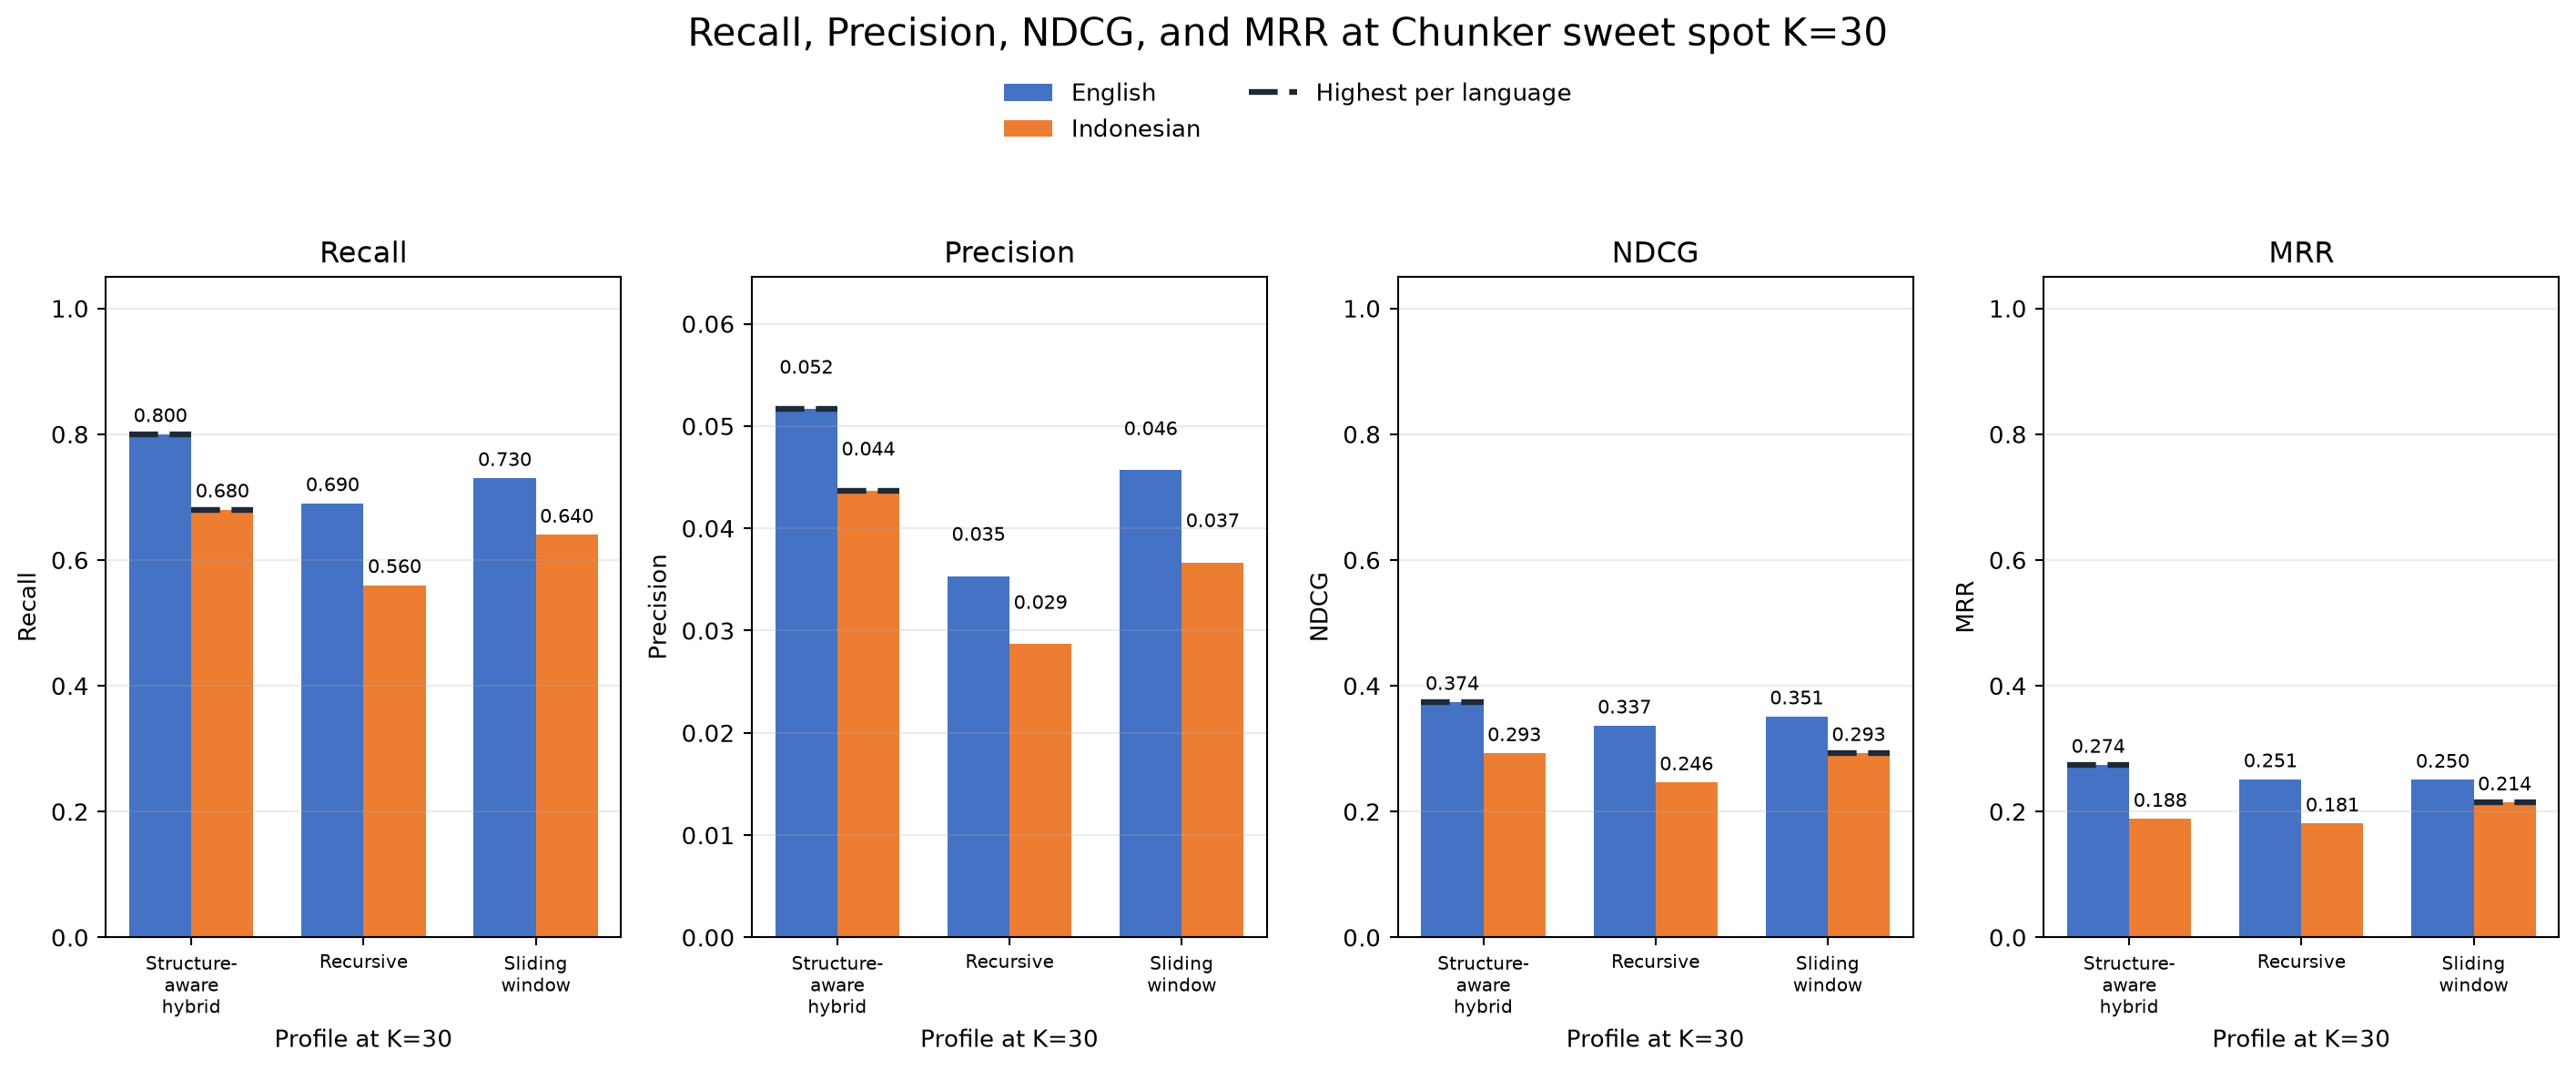
\includegraphics[width=\textwidth,height=0.52\textheight,keepaspectratio]{images/experiments/customer_service_revision/final_eda/metrics-at-sweet-spot-chunker.png}
\caption{\emph{Recall}, \emph{precision}, \emph{NDCG}, dan \emph{MRR} konfigurasi \emph{chunker} pada \(K = 30\)}
\label{fig:customer-chunker-sweet-spot}
\end{figure}

\paragraph{\emph{Generation} pada kelompok \emph{chunker}.}
\emph{Indexer} \emph{hybrid}, \emph{parser}, \emph{dataset}, \emph{embedding}, dan parameter \emph{retrieval} dipertahankan sama.
Untuk setiap strategi segmentasi, sepuluh kandidat teratas (\(K = 10\)) dikirim ke \texttt{openai/gpt-5.6-luna}
untuk 100 pertanyaan berbahasa Inggris. \emph{Cutoff} ini memisahkan fungsi dua tahap. \emph{Retrieval}
diukur sampai \(K = 30\) untuk melihat cakupan, sedangkan \emph{generation} memakai sepuluh konteks
teratas sebagai \emph{evidence} yang dibaca \emph{model}. Pada \emph{cutoff} ini, estimasi \emph{token} rata-rata adalah
3.514 untuk \emph{Structure-aware hybrid}, 3.619 untuk \emph{Recursive}, dan 5.135 untuk
\emph{Sliding-window}. \emph{Sliding-window} membawa \emph{payload} paling besar karena segmen yang berdekatan
lebih sering ikut terbawa, sedangkan \emph{hybrid} dan \emph{recursive} memiliki \emph{volume} yang lebih ringkas.
Angka tersebut adalah \emph{volume} konteks \emph{generation} dan berbeda dari \emph{payload} kandidat \(K = 30\)
yang diteruskan ke \emph{reranker}.

\emph{Correctness} mengukur kelengkapan dan kesesuaian jawaban terhadap jawaban acuan. \emph{Faithfulness}
mengukur apakah klaim yang ditulis benar-benar didukung oleh sepuluh konteks yang dikirim.
Keduanya dihitung terpisah per konfigurasi, sehingga skor tidak memperoleh \emph{evidence} dari
konfigurasi lain. Perbandingan akhir dilakukan setelah setiap strategi memiliki 100 jawaban
dan 100 penilaian.

\begin{figure}[H]
\centering
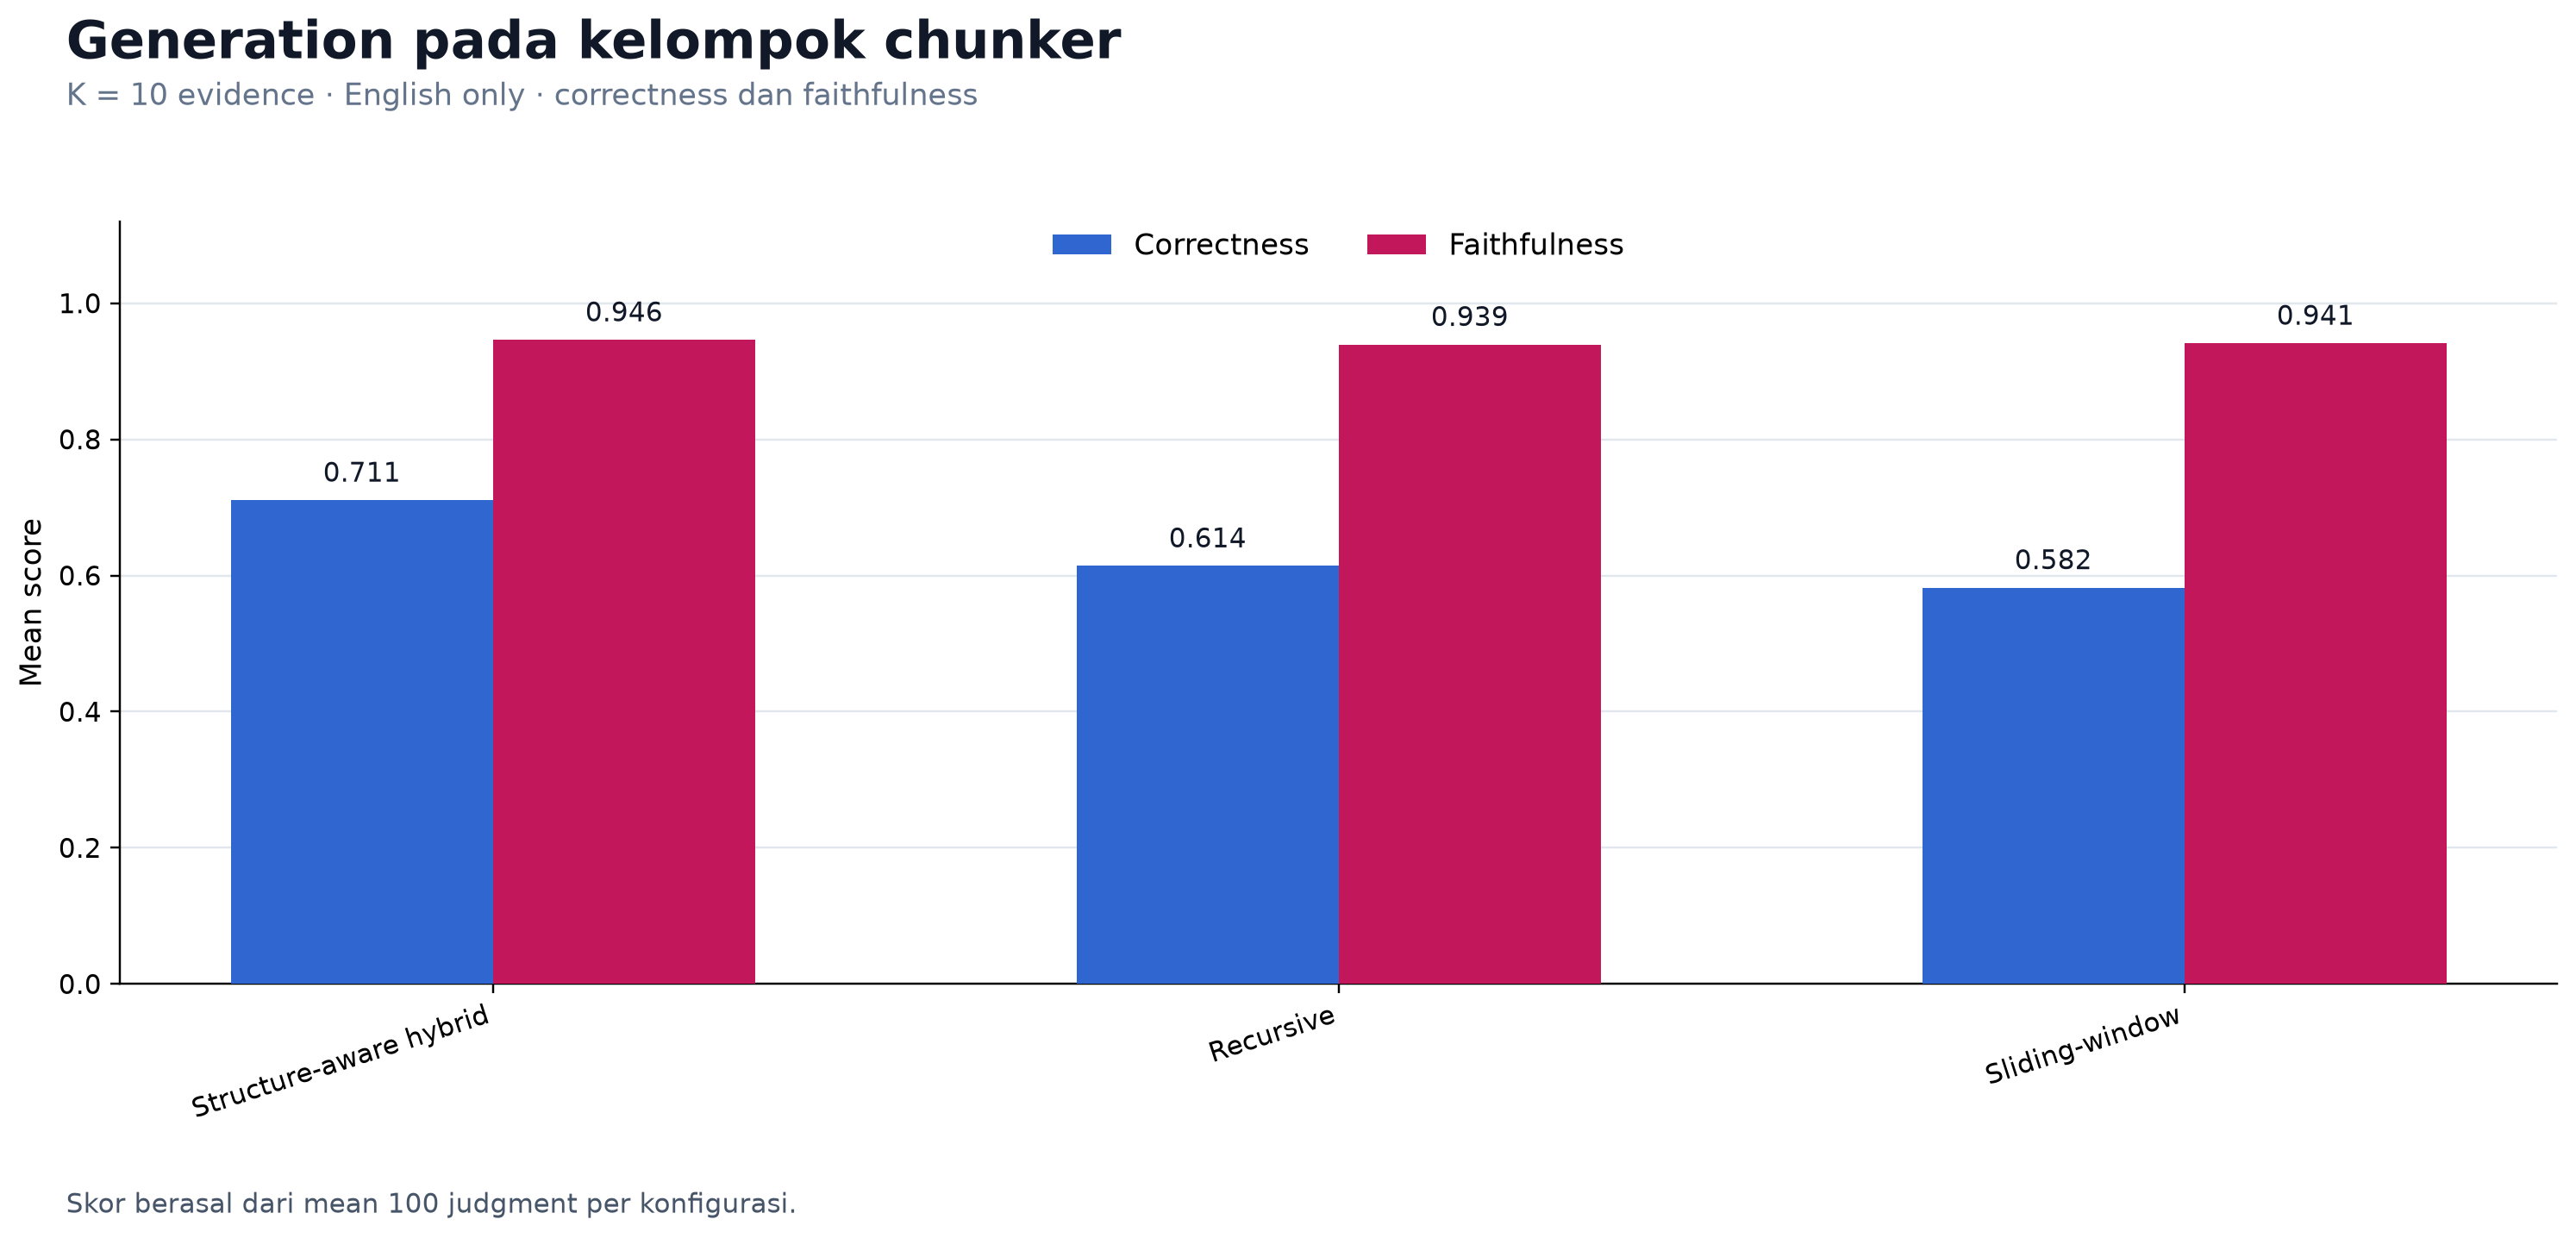
\includegraphics[width=\textwidth,height=0.43\textheight,keepaspectratio]{images/experiments/customer_service_revision/final_eda/generation-chunker.png}
\caption{\emph{Correctness} dan \emph{faithfulness} \emph{generation} pada kelompok \emph{chunker} dengan \(K = 10\)}
\label{fig:customer-chunker-generation-bar}
\end{figure}

Pada Gambar~\ref{fig:customer-chunker-generation-bar}, \emph{Structure-aware} \emph{hybrid} memperoleh
\emph{correctness} 0,711 dan \emph{faithfulness} 0,946. Hasil ini selaras dengan \emph{recall} \emph{retrieval} 0,740,
\emph{precision} 0,048, dan \emph{NDCG} 0,333 pada \(K = 30\). Dengan \emph{volume} sekitar 3.514 \emph{token}, \emph{payload}
\emph{hybrid} memberi \emph{evidence} yang cukup lengkap tanpa menjadi konfigurasi dengan \emph{volume} terbesar.

\emph{Recursive} memperoleh \emph{correctness} 0,614 dan \emph{faithfulness} 0,939. \emph{Payload} rata-ratanya hampir
sama dengan \emph{hybrid}, yaitu sekitar 3.619 \emph{token}, sehingga selisih skor tidak dapat dijelaskan
oleh \emph{volume} \emph{token} saja. \emph{Recall} \emph{recursive} yang lebih rendah, yaitu 0,625, menunjukkan bahwa
sebagian \emph{evidence} yang diperlukan belum masuk ke sepuluh kandidat teratas. Akibatnya, jawaban
dapat tetap cukup faithful terhadap konteks yang tersedia, tetapi lebih sering tidak lengkap
terhadap jawaban acuan.

\emph{Sliding-window} memiliki \emph{payload} terbesar, sekitar 5.135 \emph{token}, tetapi correctness-nya hanya
0,582 dan faithfulness-nya 0,941. \emph{Volume} tambahan tersebut terutama berasal dari konteks yang
berdekatan dan berulang, bukan \emph{reference} baru dalam jumlah yang sebanding. Hal ini konsisten
dengan \emph{recall} 0,685 dan \emph{NDCG} 0,322. Jadi, \emph{payload} yang lebih besar tidak otomatis menghasilkan
jawaban yang lebih lengkap.

\subsubsection{Strategi \emph{Indexing}}
\label{subsubsec:user-manual-indexing}

Perbandingan \emph{indexer} mempertahankan \emph{chunker} \emph{structure-aware}, \emph{parser}, \emph{dataset},
dan \emph{embedding} yang sama, lalu hanya mengganti \emph{plugin} \emph{indexer}. \emph{Sparse} ditetapkan sebagai
\emph{baseline} \emph{indexer} karena merupakan pendekatan leksikal yang paling sederhana dan paling klasik
dalam perbandingan. Dengan demikian, perubahan
hasil dapat dibaca sebagai dampak cara pencarian dalam menempatkan \emph{context reference} pada
kandidat awal. \emph{Dense} mengukur kedekatan makna, \emph{sparse} mengandalkan kecocokan istilah,
sedangkan \emph{hybrid} menggabungkan kedua sinyal tersebut. Konfigurasi diringkas pada
Tabel~\ref{tab:customer-indexer-config}.

\begin{table}[H]
\centering
\scriptsize
\caption{Konfigurasi \emph{indexer} pada eksperimen \emph{User Manual}}
\label{tab:customer-indexer-config}
\begin{tabularx}{\textwidth}{@{}>{\RaggedRight\arraybackslash}p{3.1cm}>{\RaggedRight\arraybackslash}p{4.2cm}>{\RaggedRight\arraybackslash}X@{}}
\toprule
\textbf{Strategi} & \textbf{\emph{Plugin}} & \textbf{Konfigurasi utama}\\
\midrule
\emph{Hybrid} & \texttt{hybrid-semantic-keyword} & \emph{Dense} \texttt{BAAI/bge-m3} dan \emph{lexical} \texttt{lexical\_text} serta \texttt{content}\\
\emph{Baseline indexer: Sparse} & \texttt{sparse-keyword} & Pencocokan \emph{lexical} pada \texttt{lexical\_text} dan \texttt{content}\\
\emph{Dense} & \texttt{dense-semantic} & Representasi \emph{dense} dari \texttt{BAAI/bge-m3}\\
\bottomrule
\end{tabularx}
\end{table}

Pertanyaan pada \emph{dataset} tidak selalu menyalin kalimat manual. Sebagian pertanyaan menyebut
gejala atau tujuan dengan bahasa sehari-hari, sementara manual menggunakan istilah produk dan
langkah teknis. Karena itu, perbandingan ini menguji apakah pencarian dapat menemukan parafrasa
sekaligus pertanyaan yang memiliki kecocokan kata langsung. Setiap kurva pada gambar berikut
dibentuk dari hasil pencatatan \emph{retrieval} yang sama untuk 200 pertanyaan, pada \emph{cutoff} \(K = 5, 10, \ldots, 60\).
Panel Inggris dan Indonesia dihitung terpisah, sedangkan nilai gabungan memakai seluruh baris
pertanyaan. \emph{Recall} menjadi dasar pemilihan konfigurasi, sementara \emph{precision}, \emph{NDCG}, dan \emph{MRR}
digunakan untuk membaca kepadatan serta posisi hasil.

\begin{figure}[H]
\centering
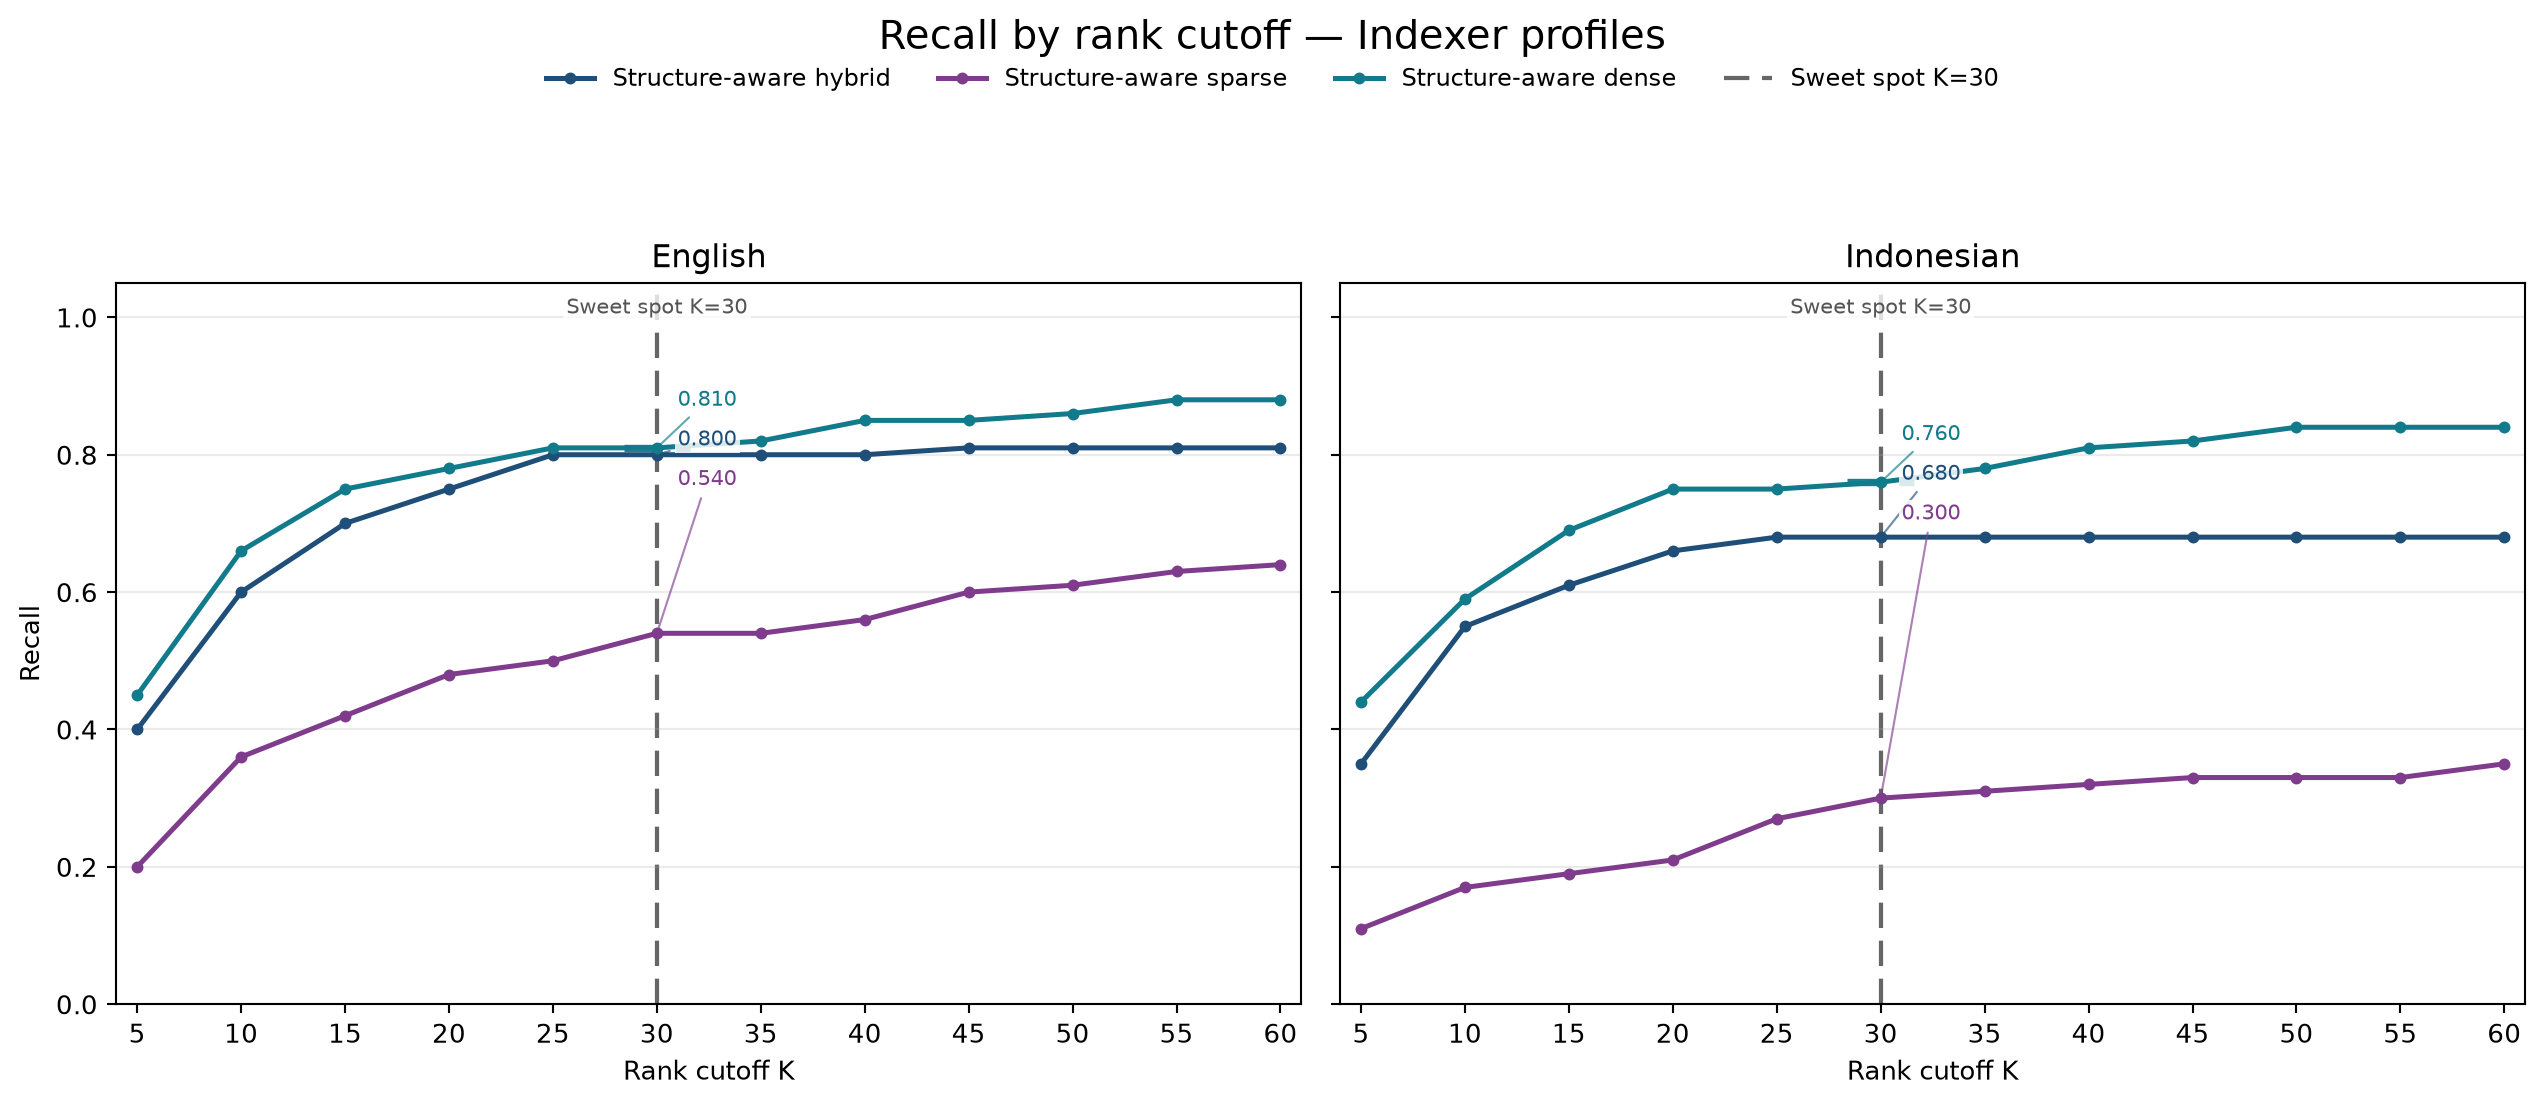
\includegraphics[width=\textwidth,height=0.52\textheight,keepaspectratio]{images/experiments/customer_service_revision/final_eda/recall-indexer.png}
\caption{Kurva \emph{context reference} \emph{recall} menurut \emph{cutoff} untuk konfigurasi \emph{indexer}}
\label{fig:customer-indexer-recall}
\end{figure}

Pada Gambar~\ref{fig:customer-indexer-recall}, ketiga kurva naik tajam pada \emph{cutoff} awal karena
kandidat tambahan masih sering membawa \emph{context reference} baru. Pada \(K = 10\), \emph{recall}
gabungan mencapai 0,625 untuk \emph{Structure-aware dense}, 0,575 untuk \emph{hybrid}, dan 0,265
untuk \emph{sparse}. Pada \(K = 30\), nilainya menjadi 0,785, 0,740, dan 0,420. Dengan demikian,
kenaikan dari \(K = 10\) ke \(K = 30\) masing-masing adalah 0,160, 0,165, dan 0,155. \emph{Dense}
berada di atas dua konfigurasi lain sejak \emph{cutoff} awal karena kedekatan makna membantu ketika
pertanyaan memakai parafrasa.

Setelah \(K = 30\), bentuk kurva mulai berbeda. \emph{Hybrid} hanya naik menjadi 0,745 pada \(K = 60\),
sedangkan \emph{dense} naik menjadi 0,860 dan \emph{sparse} menjadi 0,495. Artinya, \(K = 30\) sudah menjadi
\emph{plateau} untuk \emph{hybrid}, tetapi belum menjadi \emph{plateau} penuh untuk \emph{dense} dan \emph{sparse}. \(K = 30\) tetap
digunakan sebagai \emph{cutoff} bersama karena memberikan anggaran kandidat yang sama untuk seluruh
komponen dan membatasi beban tahap \emph{downstream}. Nilai \(K = 60\) dipertahankan sebagai \emph{sweep}
sensitivitas untuk menunjukkan cakupan tambahan yang masih dapat diperoleh, bukan sebagai \emph{cutoff}
\emph{generation}.

Perbedaan \emph{dense} dan \emph{sparse} juga terlihat pada bahasa. Pada \(K = 30\), \emph{dense} mencapai \emph{recall}
0,810 untuk Inggris dan 0,760 untuk Indonesia, sehingga selisihnya 0,050. \emph{Hybrid} mencapai
0,800 dan 0,680 dengan selisih 0,120, sedangkan \emph{sparse} hanya 0,540 dan 0,300 dengan selisih
0,240. Selisih yang lebih besar pada \emph{sparse} menunjukkan bahwa kecocokan istilah langsung lebih
mudah berubah ketika bahasa pertanyaan berubah. \emph{Dense} lebih tahan terhadap perubahan kosakata
karena pencocokan utamanya menggunakan kedekatan makna.

\begin{figure}[H]
\centering
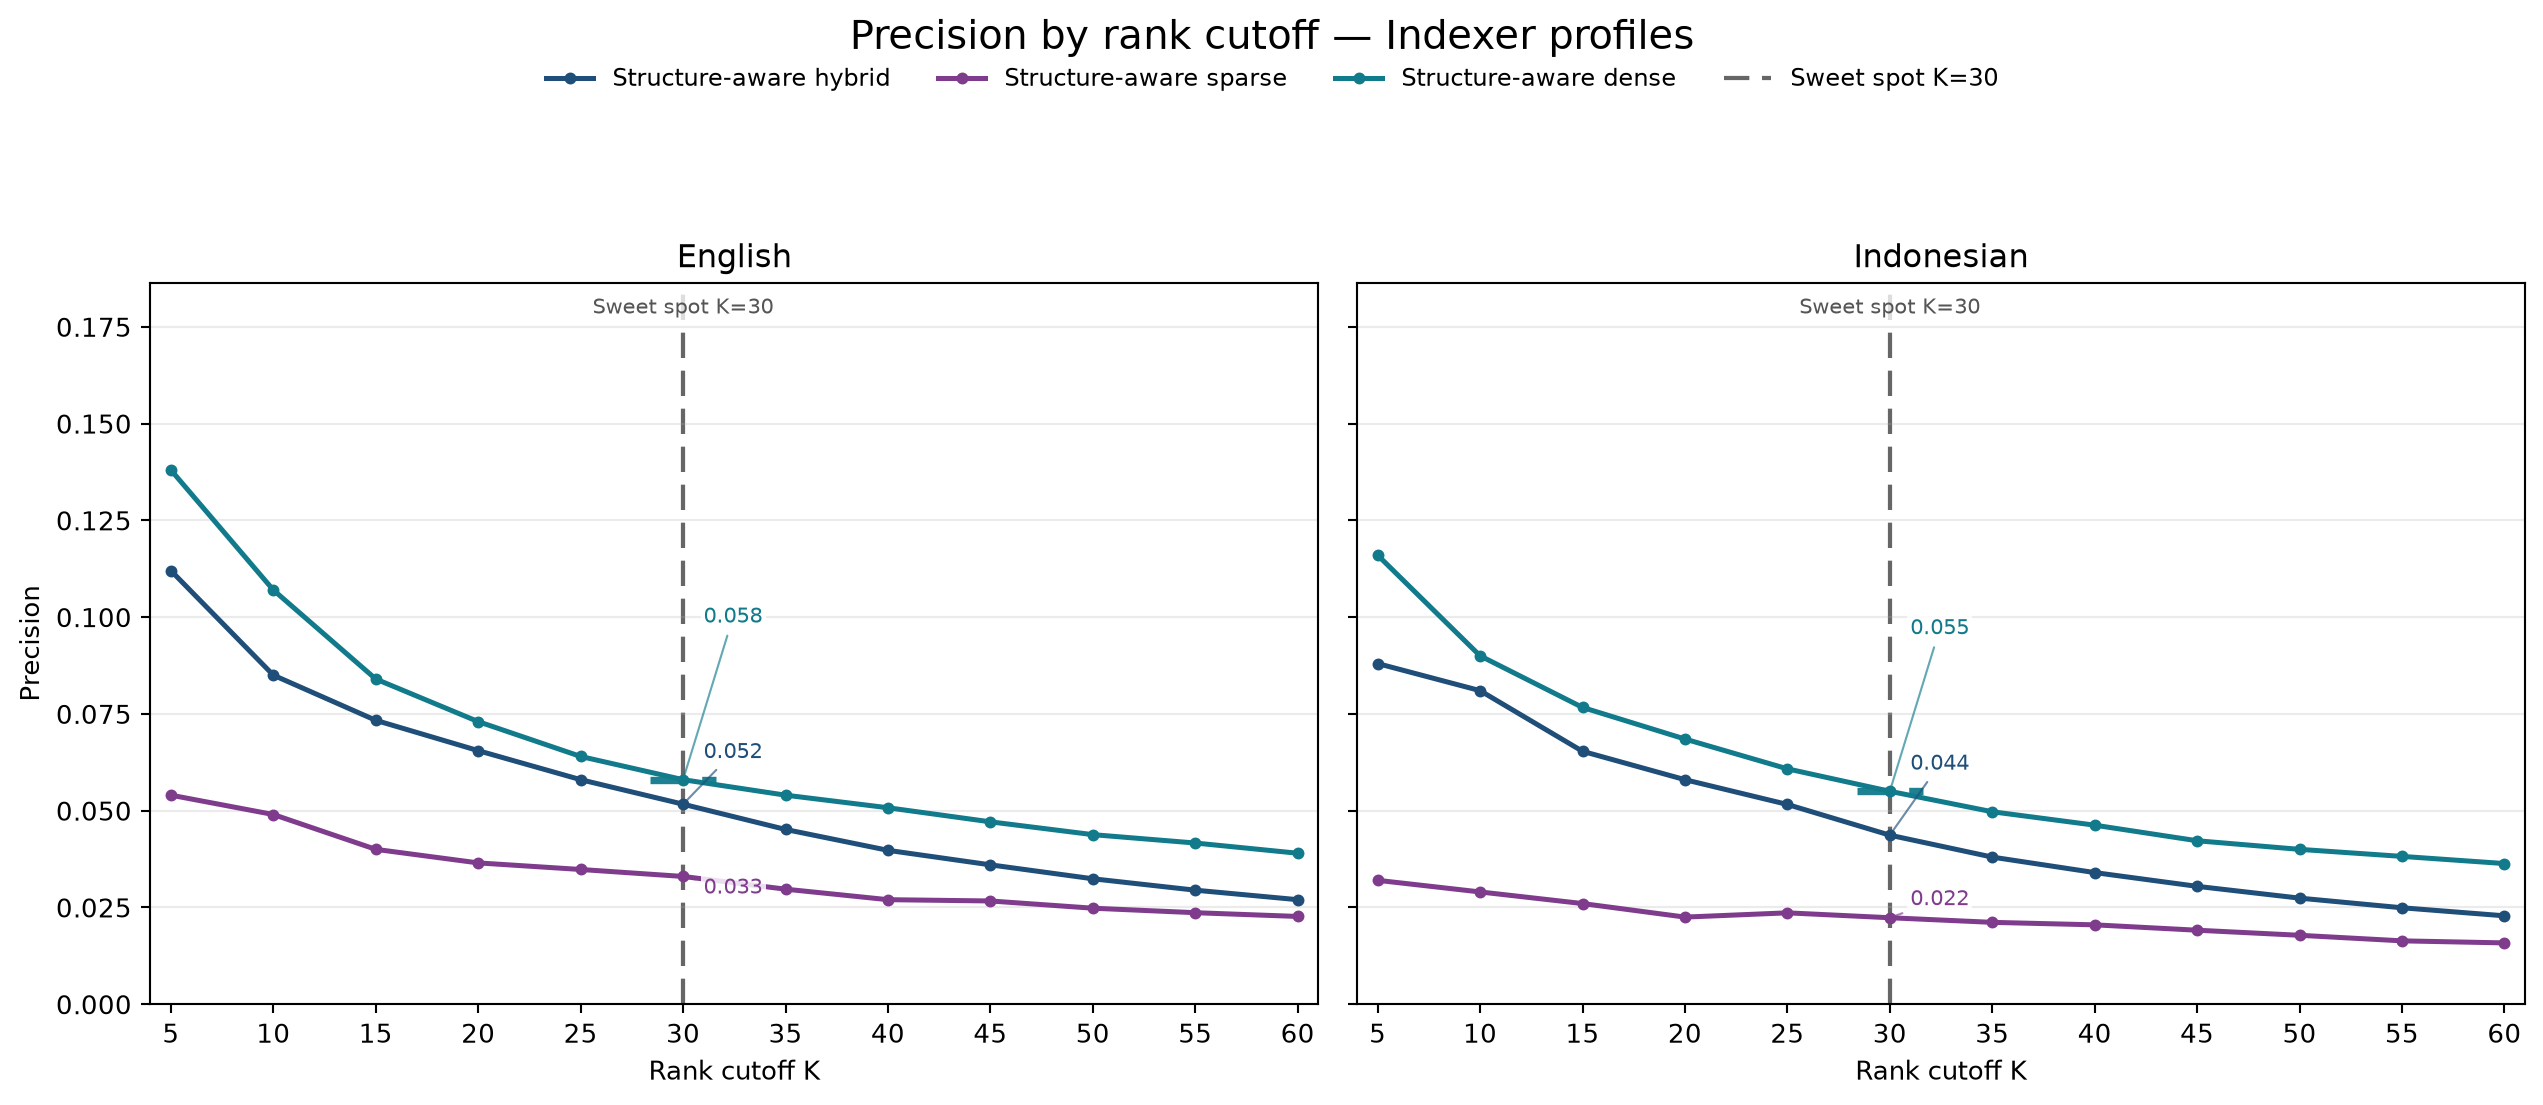
\includegraphics[width=\textwidth,height=0.52\textheight,keepaspectratio]{images/experiments/customer_service_revision/final_eda/precision-indexer.png}
\caption{Kurva \emph{context reference} \emph{precision} menurut \emph{cutoff} untuk konfigurasi \emph{indexer}}
\label{fig:customer-indexer-precision}
\end{figure}

Pada Gambar~\ref{fig:customer-indexer-precision}, \emph{precision} turun ketika \emph{cutoff} diperbesar
karena kandidat baru menambah penyebut lebih cepat daripada jumlah \emph{reference} baru. Pada \(K = 10\),
\emph{precision} \emph{dense}, \emph{hybrid}, dan \emph{sparse} masing-masing 0,098, 0,083, dan 0,039. Pada \(K = 30\),
nilainya menjadi 0,057, 0,048, dan 0,028, lalu turun lagi menjadi 0,038, 0,025, dan 0,019
pada \(K = 60\). \emph{Dense} tetap paling padat karena kandidat di bagian atas lebih sering memiliki
hubungan makna dengan pertanyaan. \emph{Sparse} lebih cepat turun karena kecocokan kata yang lemah
menambah kandidat yang tidak membawa \emph{reference} baru. Penurunan ini adalah konsekuensi dari
memperluas cakupan, bukan berarti \emph{reference} yang sudah ditemukan hilang.

\begin{figure}[H]
\centering
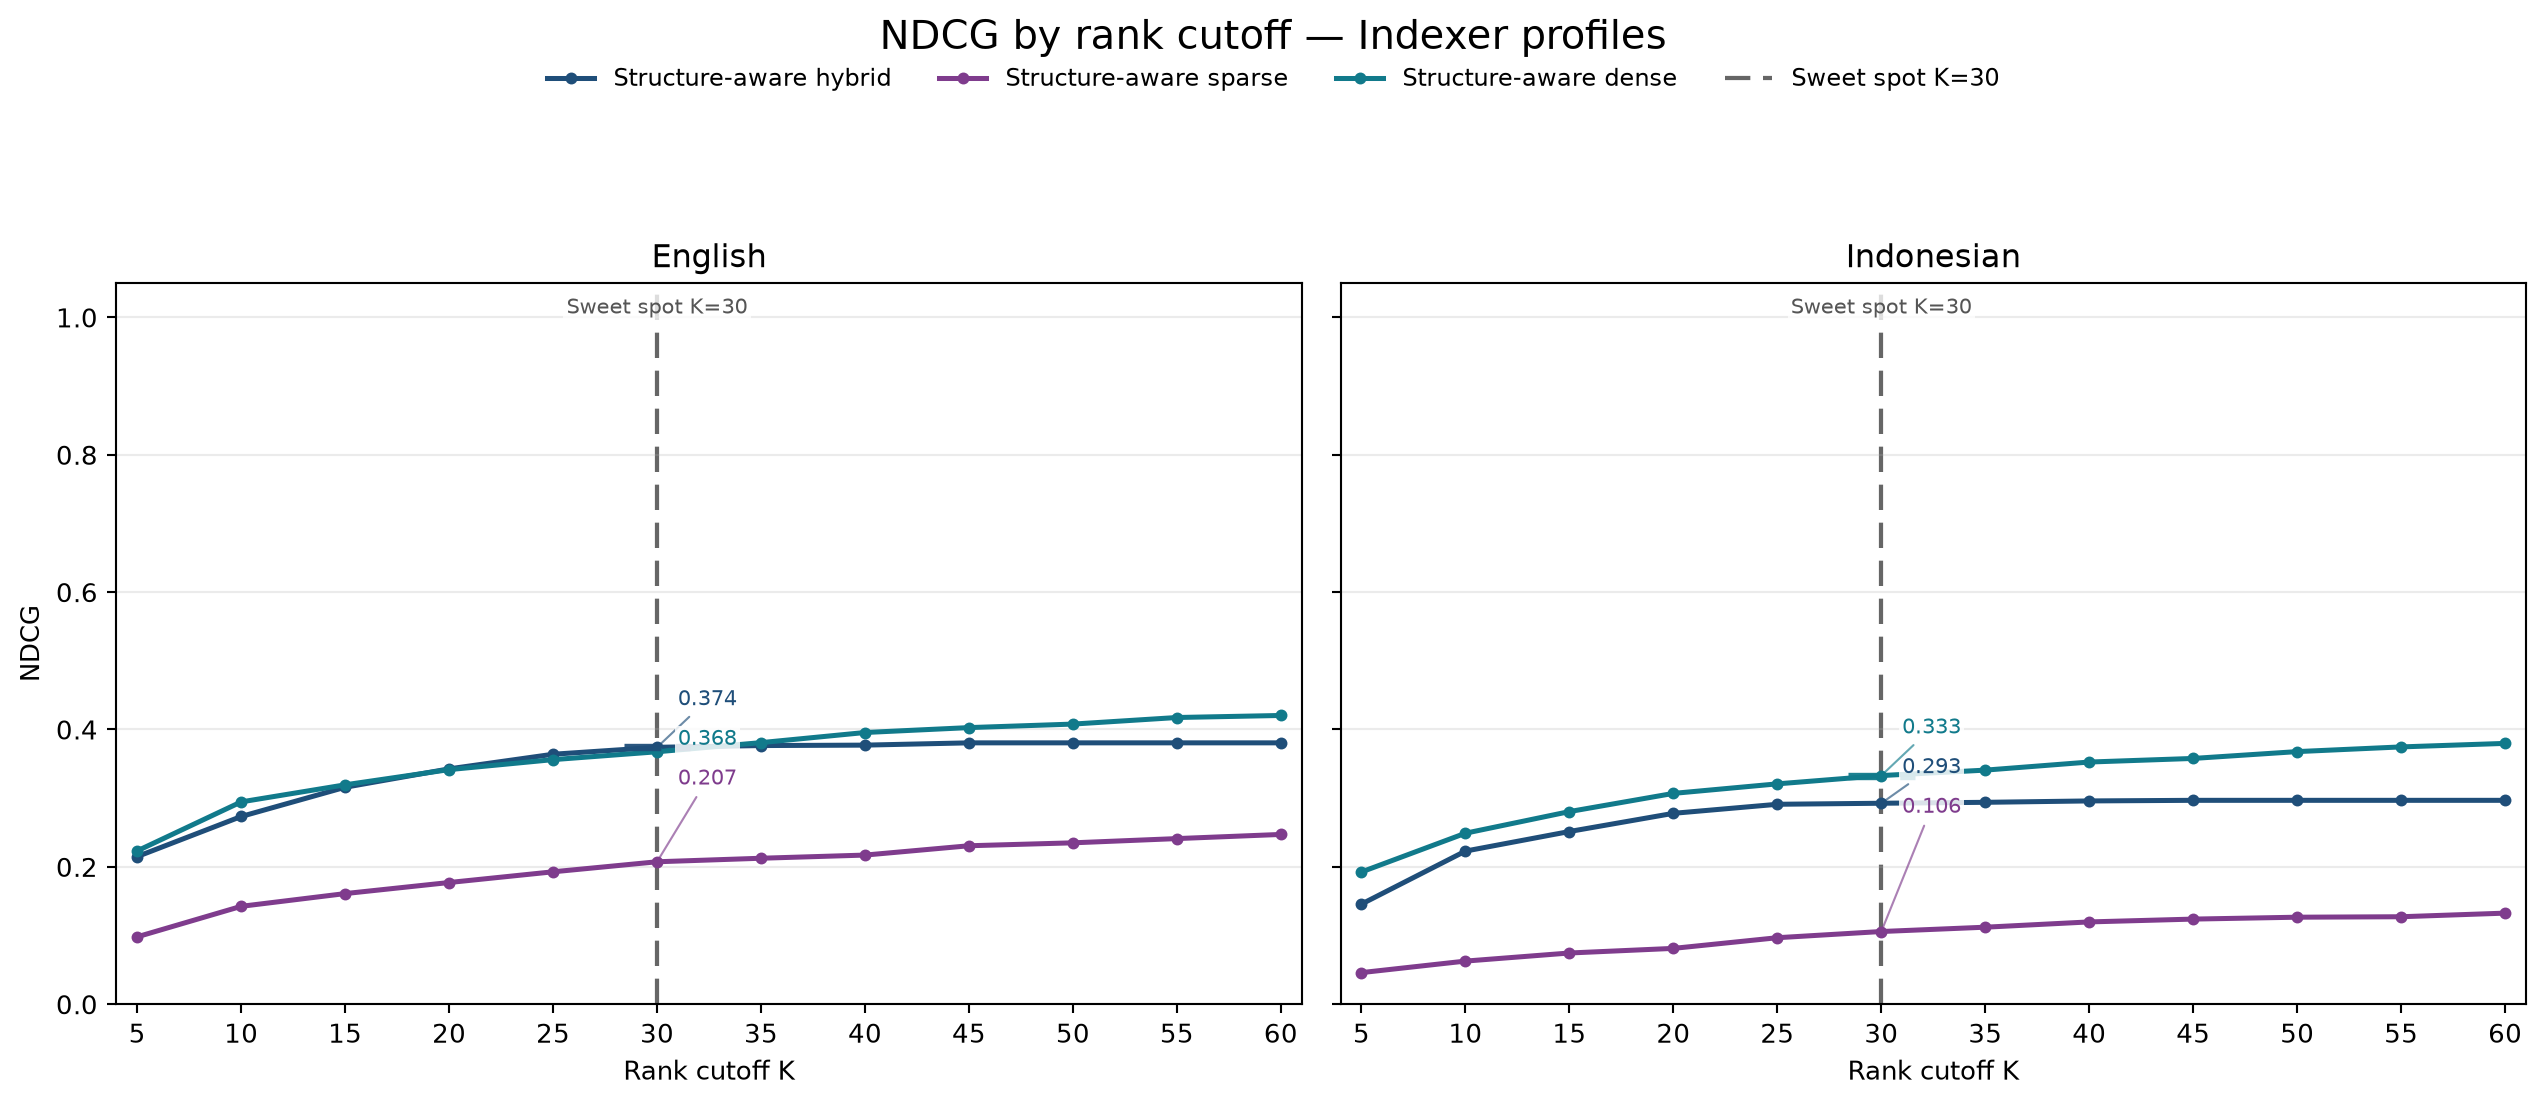
\includegraphics[width=\textwidth,height=0.52\textheight,keepaspectratio]{images/experiments/customer_service_revision/final_eda/ndcg-indexer.png}
\caption{Kurva \emph{NDCG} menurut \emph{cutoff} untuk konfigurasi \emph{indexer}}
\label{fig:customer-indexer-ndcg}
\end{figure}

Pada Gambar~\ref{fig:customer-indexer-ndcg}, \emph{NDCG} pada \(K = 10\) adalah 0,272 untuk \emph{dense},
0,248 untuk \emph{hybrid}, dan 0,103 untuk \emph{sparse}. Pada \(K = 30\), nilainya menjadi 0,350, 0,333,
dan 0,157. \emph{Dense} kemudian mencapai 0,400 pada \(K = 60\), sedangkan \emph{hybrid} dan \emph{sparse} mencapai
0,339 dan 0,190. Kenaikan \emph{dense} dari \(K = 30\) ke \(K = 60\) sebesar 0,050 menunjukkan bahwa
\emph{reference} tambahan tidak hanya ditemukan, tetapi juga masuk pada posisi yang cukup baik. \emph{Sparse}
tetap rendah karena kecocokan kata yang lemah lebih sering menunda \emph{reference} di dalam \emph{ranking}.

\begin{figure}[H]
\centering
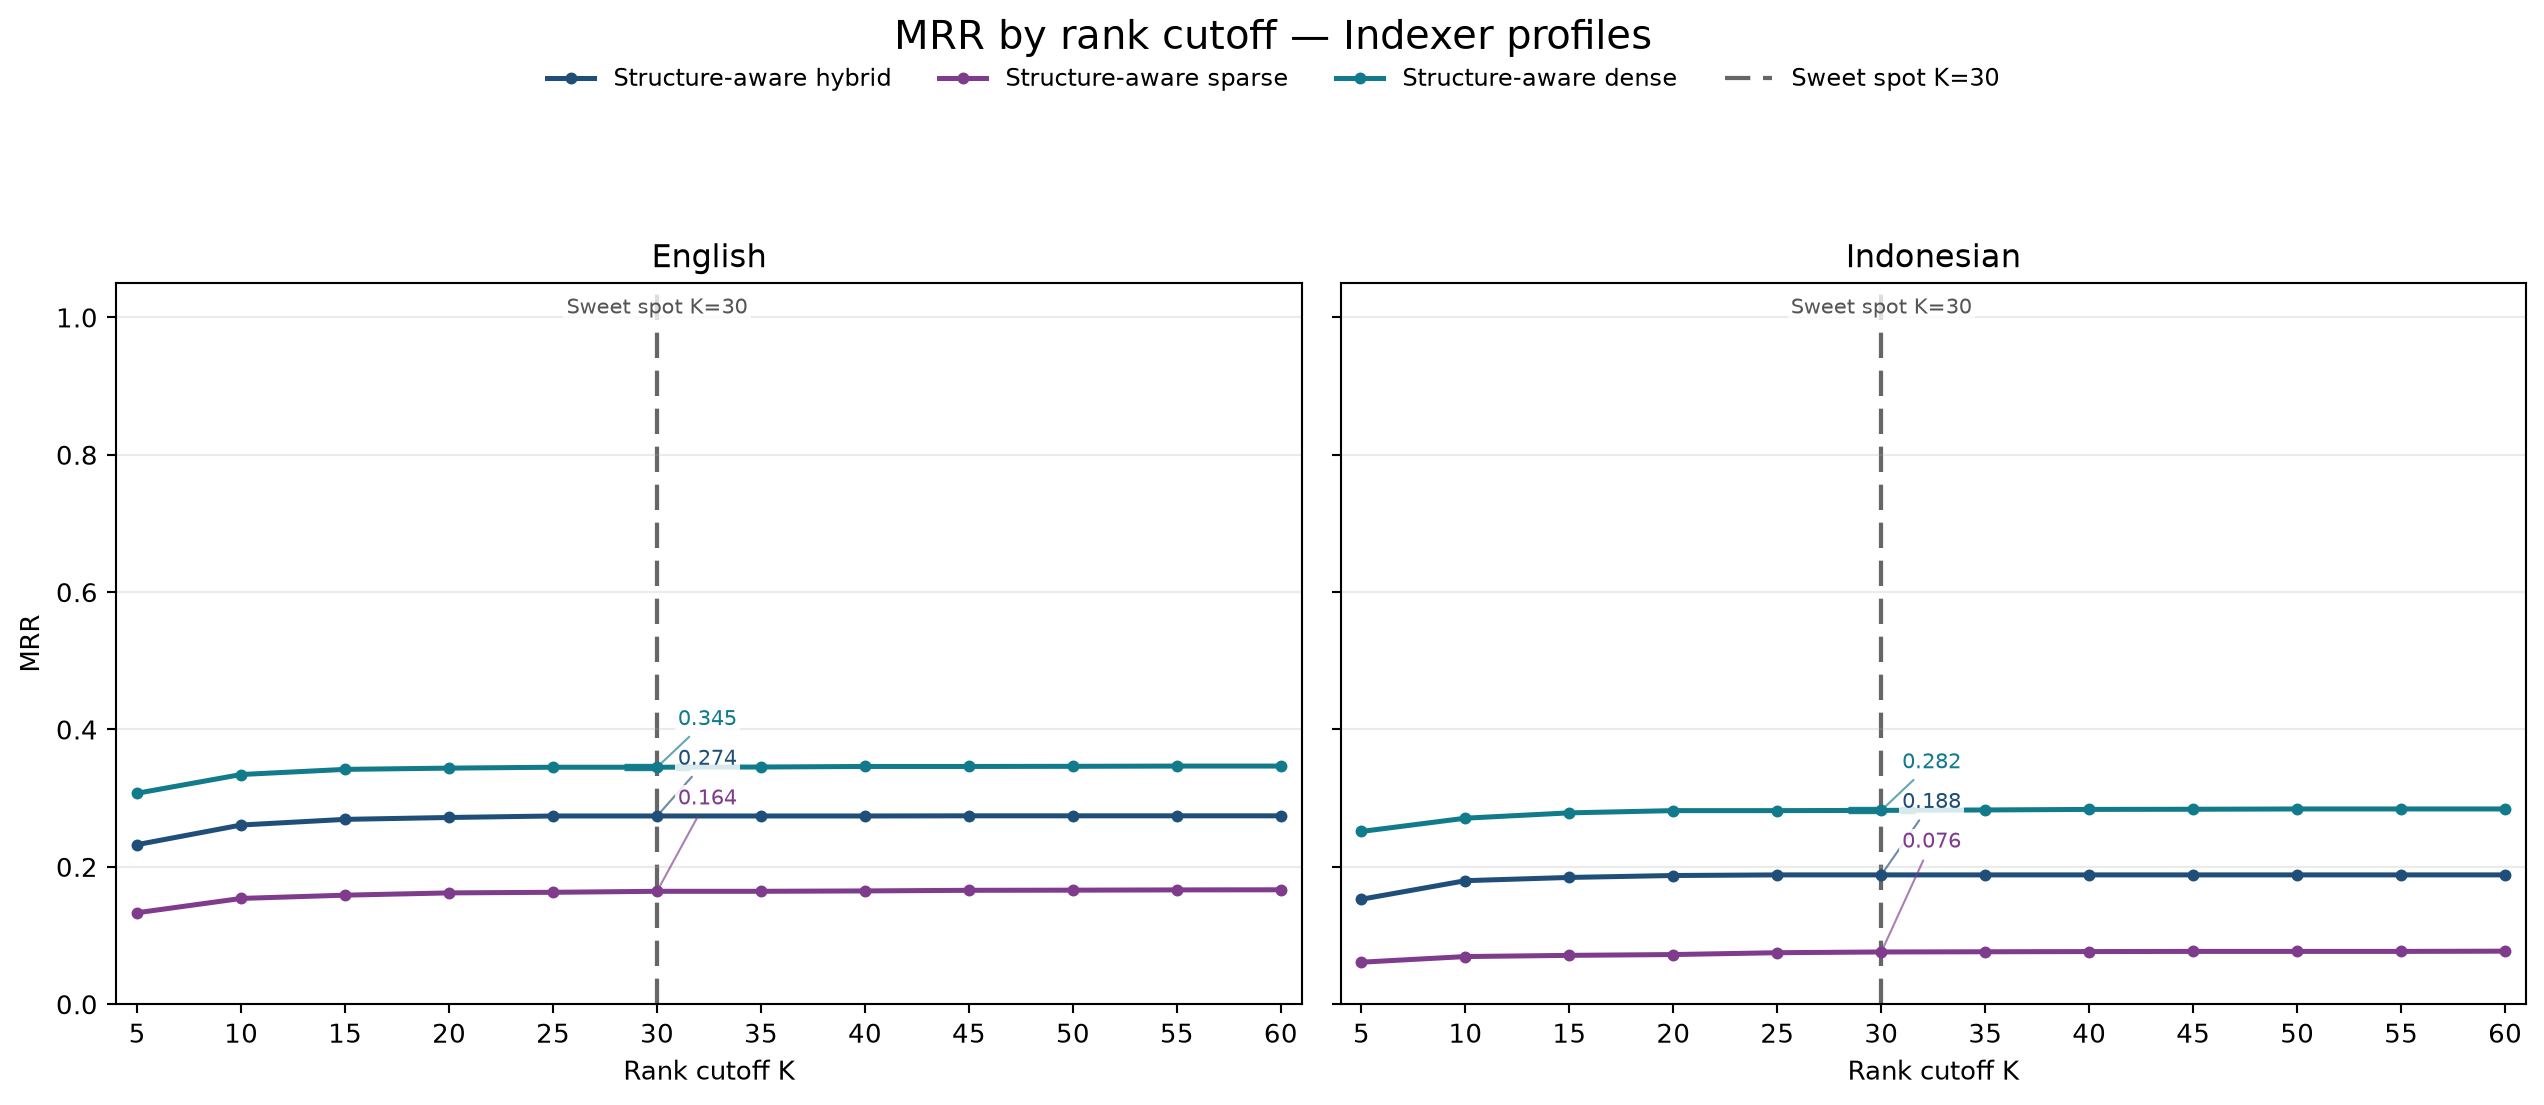
\includegraphics[width=\textwidth,height=0.52\textheight,keepaspectratio]{images/experiments/customer_service_revision/final_eda/mrr-indexer.png}
\caption{Kurva \emph{MRR} menurut \emph{cutoff} untuk konfigurasi \emph{indexer}}
\label{fig:customer-indexer-mrr}
\end{figure}

Pada Gambar~\ref{fig:customer-indexer-mrr}, \emph{MRR} pada \(K = 30\) adalah 0,314 untuk \emph{dense},
0,231 untuk \emph{hybrid}, dan 0,120 untuk \emph{sparse}. \emph{Dense} berarti lebih sering menempatkan \emph{reference}
pertama di peringkat awal. Pada \(K = 60\), \emph{MRR} hanya berubah menjadi 0,315, 0,231, dan 0,122.
Dengan demikian, tambahan kandidat setelah \(K = 30\) terutama memperpanjang ekor \emph{ranking} dan
tidak banyak mengubah posisi \emph{reference} pertama.

\begin{figure}[H]
\centering
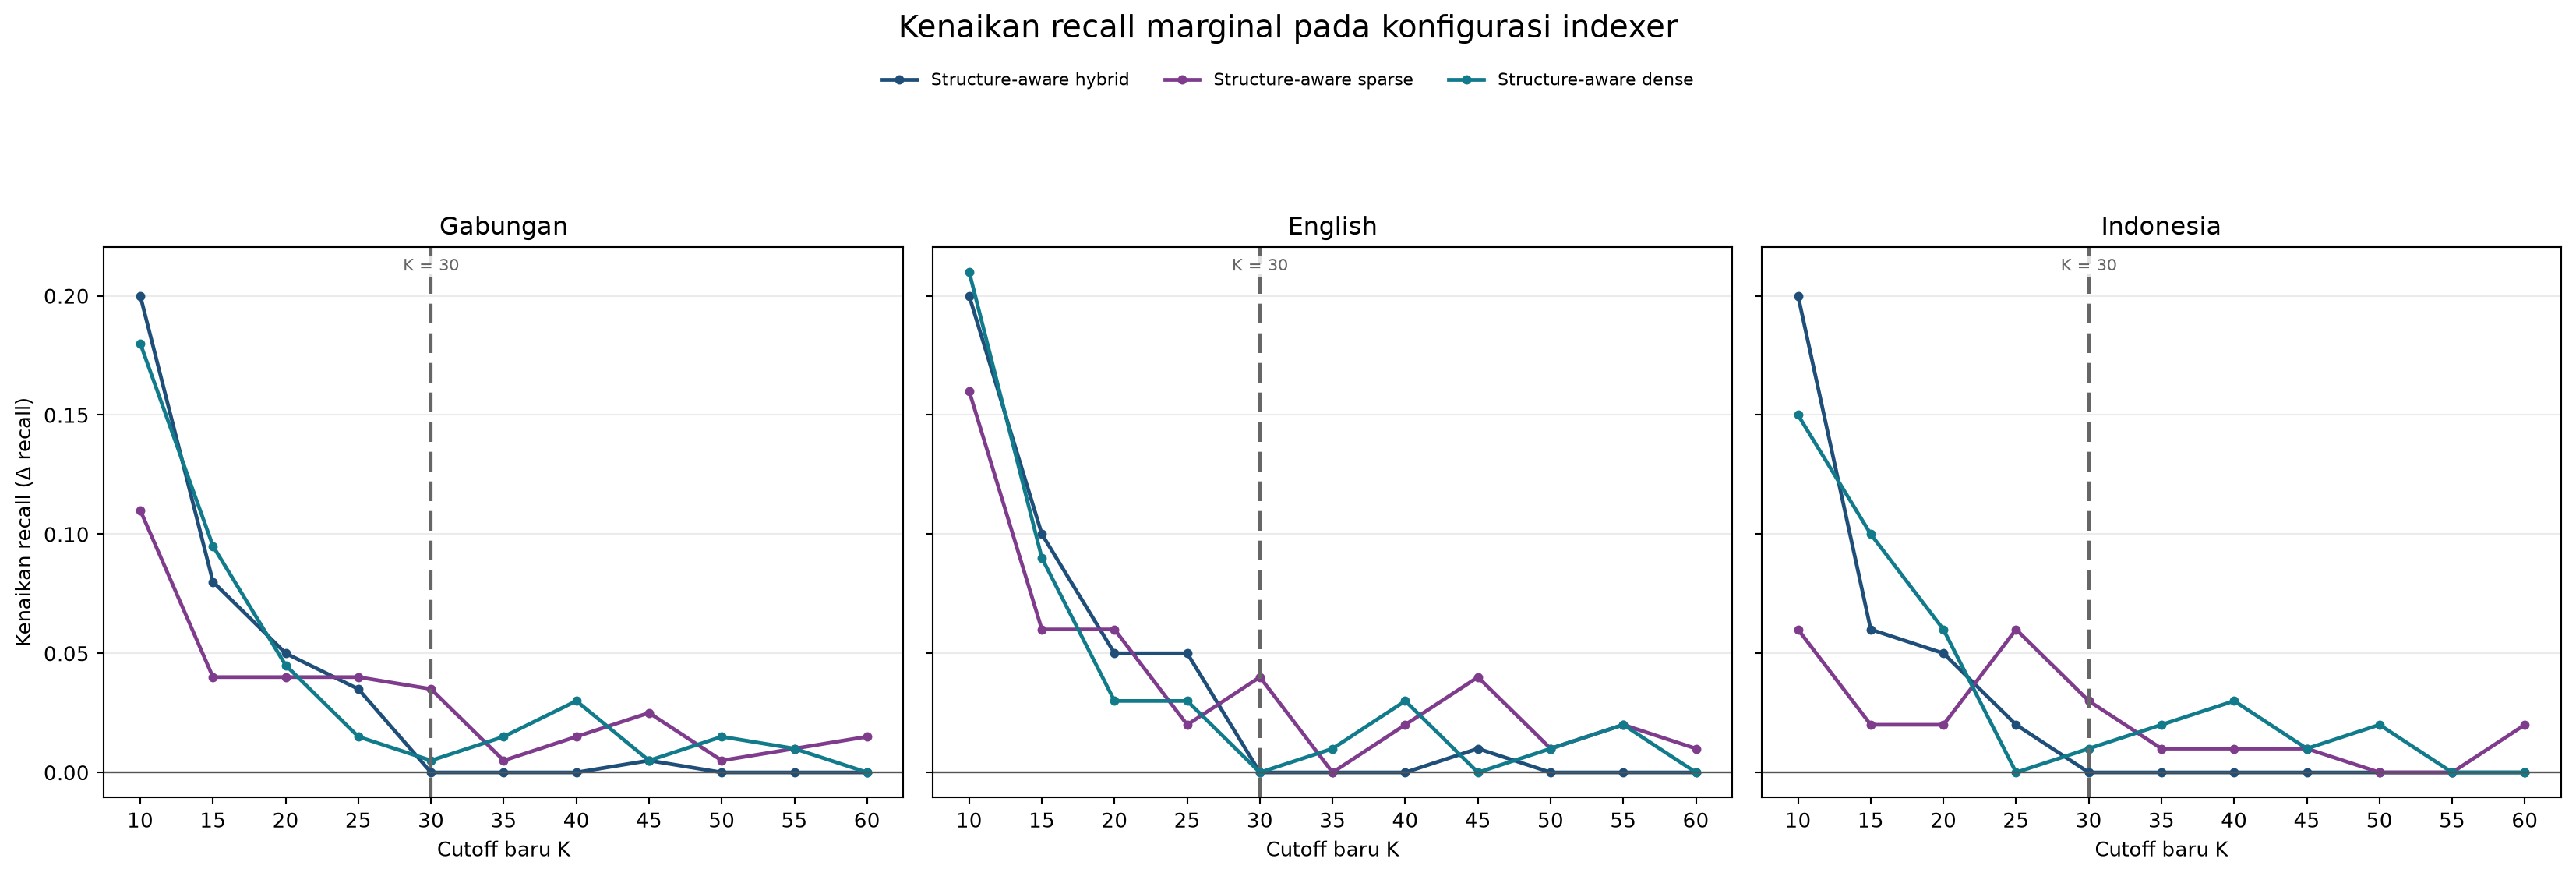
\includegraphics[width=\textwidth,height=0.43\textheight,keepaspectratio]{images/experiments/customer_service_revision/final_eda/recall-marginal-delta-indexer.png}
\caption{Tambahan \emph{recall} pada setiap kenaikan \emph{cutoff} untuk konfigurasi \emph{indexer}}
\label{fig:customer-indexer-recall-delta}
\end{figure}

Gambar~\ref{fig:customer-indexer-recall-delta} memperjelas mengapa satu \emph{cutoff} bersama tetap
diperlukan. Pada kenaikan dari \(K = 5\) ke \(K = 10\), tambahan \emph{recall} gabungan adalah 0,200
untuk \emph{hybrid}, 0,110 untuk \emph{sparse}, dan 0,180 untuk \emph{dense}. Pada kenaikan \(K = 25\) ke \(K = 30\),
\emph{hybrid} hanya bertambah 0,000, \emph{sparse} 0,035, dan \emph{dense} 0,005. Setelah \(K = 30\), \emph{dense} dan
\emph{sparse} masih memperoleh tambahan bertahap hingga total 0,075 pada \(K = 60\), sedangkan \emph{hybrid}
hanya bertambah 0,005. Jadi, \(K = 30\) bukan titik ketika semua konfigurasi telah berhenti
bertambah. Titik ini dipakai sebagai kompromi yang konsisten untuk seluruh konfigurasi, sementara
kurva sampai \(K = 60\) menunjukkan batas cakupan yang mungkin diperoleh jika biaya kandidat
ditambah.

\begin{table}[H]
\centering
\scriptsize
\caption{Hasil strategi \emph{indexing} pada \emph{sweet spot} (K = 30)}
\label{tab:customer-indexing-results}
\begin{tabularx}{\textwidth}{@{}>{\RaggedRight\arraybackslash}p{3.7cm} r r r r r@{}}
\toprule
\textbf{Strategi} & \textbf{K} & \textbf{\emph{Recall}} & \textbf{\emph{Precision}} & \textbf{\emph{NDCG}} & \textbf{\emph{MRR}}\\
\midrule
\emph{Structure-aware hybrid} & 30 & 0,740 & 0,048 & 0,333 & 0,231\\
\emph{Baseline indexer: Structure-aware sparse} & 30 & 0,420 & 0,028 & 0,157 & 0,120\\
\emph{Structure-aware dense} & 30 & \textbf{0,785} & \textbf{0,057} & \textbf{0,350} & \textbf{0,314}\\
\bottomrule
\end{tabularx}
\end{table}

Pada \(K = 30\), \emph{dense} memperoleh \emph{recall} 0,785, \emph{precision} 0,057, \emph{NDCG} 0,350, dan \emph{MRR} 0,314.
\emph{Hybrid} berada di bawahnya dengan 0,740, 0,048, 0,333, dan 0,231. \emph{Sparse} memperoleh 0,420,
0,028, 0,157, dan 0,120. \emph{Structure-aware} \emph{dense} mengalahkan \emph{baseline} \emph{Sparse} dengan \emph{recall}
0,785 berbanding 0,420, yaitu delta +0,365. \emph{Structure-aware} \emph{hybrid} juga mengalahkan \emph{baseline}
tersebut dengan \emph{recall} 0,740, yaitu delta +0,320. Dibandingkan \emph{hybrid}, \emph{dense} menambah 0,045 \emph{recall}, 0,009 \emph{precision},
0,017 \emph{NDCG}, dan 0,083 \emph{MRR}. Dibandingkan \emph{sparse}, selisihnya menjadi 0,365 \emph{recall}, 0,029
\emph{precision}, 0,193 \emph{NDCG}, dan 0,194 \emph{MRR}. Jadi \emph{dense} bukan hanya menemukan lebih banyak \emph{reference},
tetapi juga menempatkan \emph{reference} pertama dan \emph{reference} relevan lebih awal.

Keunggulan \emph{dense} paling masuk akal pada pertanyaan yang memparafrasekan istilah manual atau
menyebut gejala dan tujuan tanpa menyalin nama fitur. \emph{Hybrid} tetap kompetitif karena masih dapat
memanfaatkan istilah yang sama, tetapi tambahan sinyal \emph{lexical} tidak meningkatkan cakupan
sebanyak \emph{dense} pada \emph{dataset} ini. \emph{Sparse} paling sensitif terhadap perbedaan kata, sehingga
tertinggal terutama pada pertanyaan gejala, tujuan, dan pertanyaan bahasa Indonesia.

Rincian bahasa memperlihatkan pola yang sama. Pada \(K = 30\), \emph{structure-aware} \emph{dense} memperoleh
\emph{recall} Inggris dan Indonesia 0,810 dan 0,760. \emph{Hybrid} memperoleh 0,800 dan 0,680, sedangkan
\emph{sparse} 0,540 dan 0,300. Selisih \emph{dense} hanya 0,050, sementara selisih \emph{sparse} mencapai 0,240.
Hal ini menunjukkan bahwa \emph{BGE-M3} lebih mampu mempertahankan kedekatan makna lintas bahasa.
Dengan \emph{recall} sebagai dasar pemilihan, \emph{structure-aware} \emph{dense} dipilih sebagai \emph{indexer} acuan.

\begin{figure}[H]
\centering
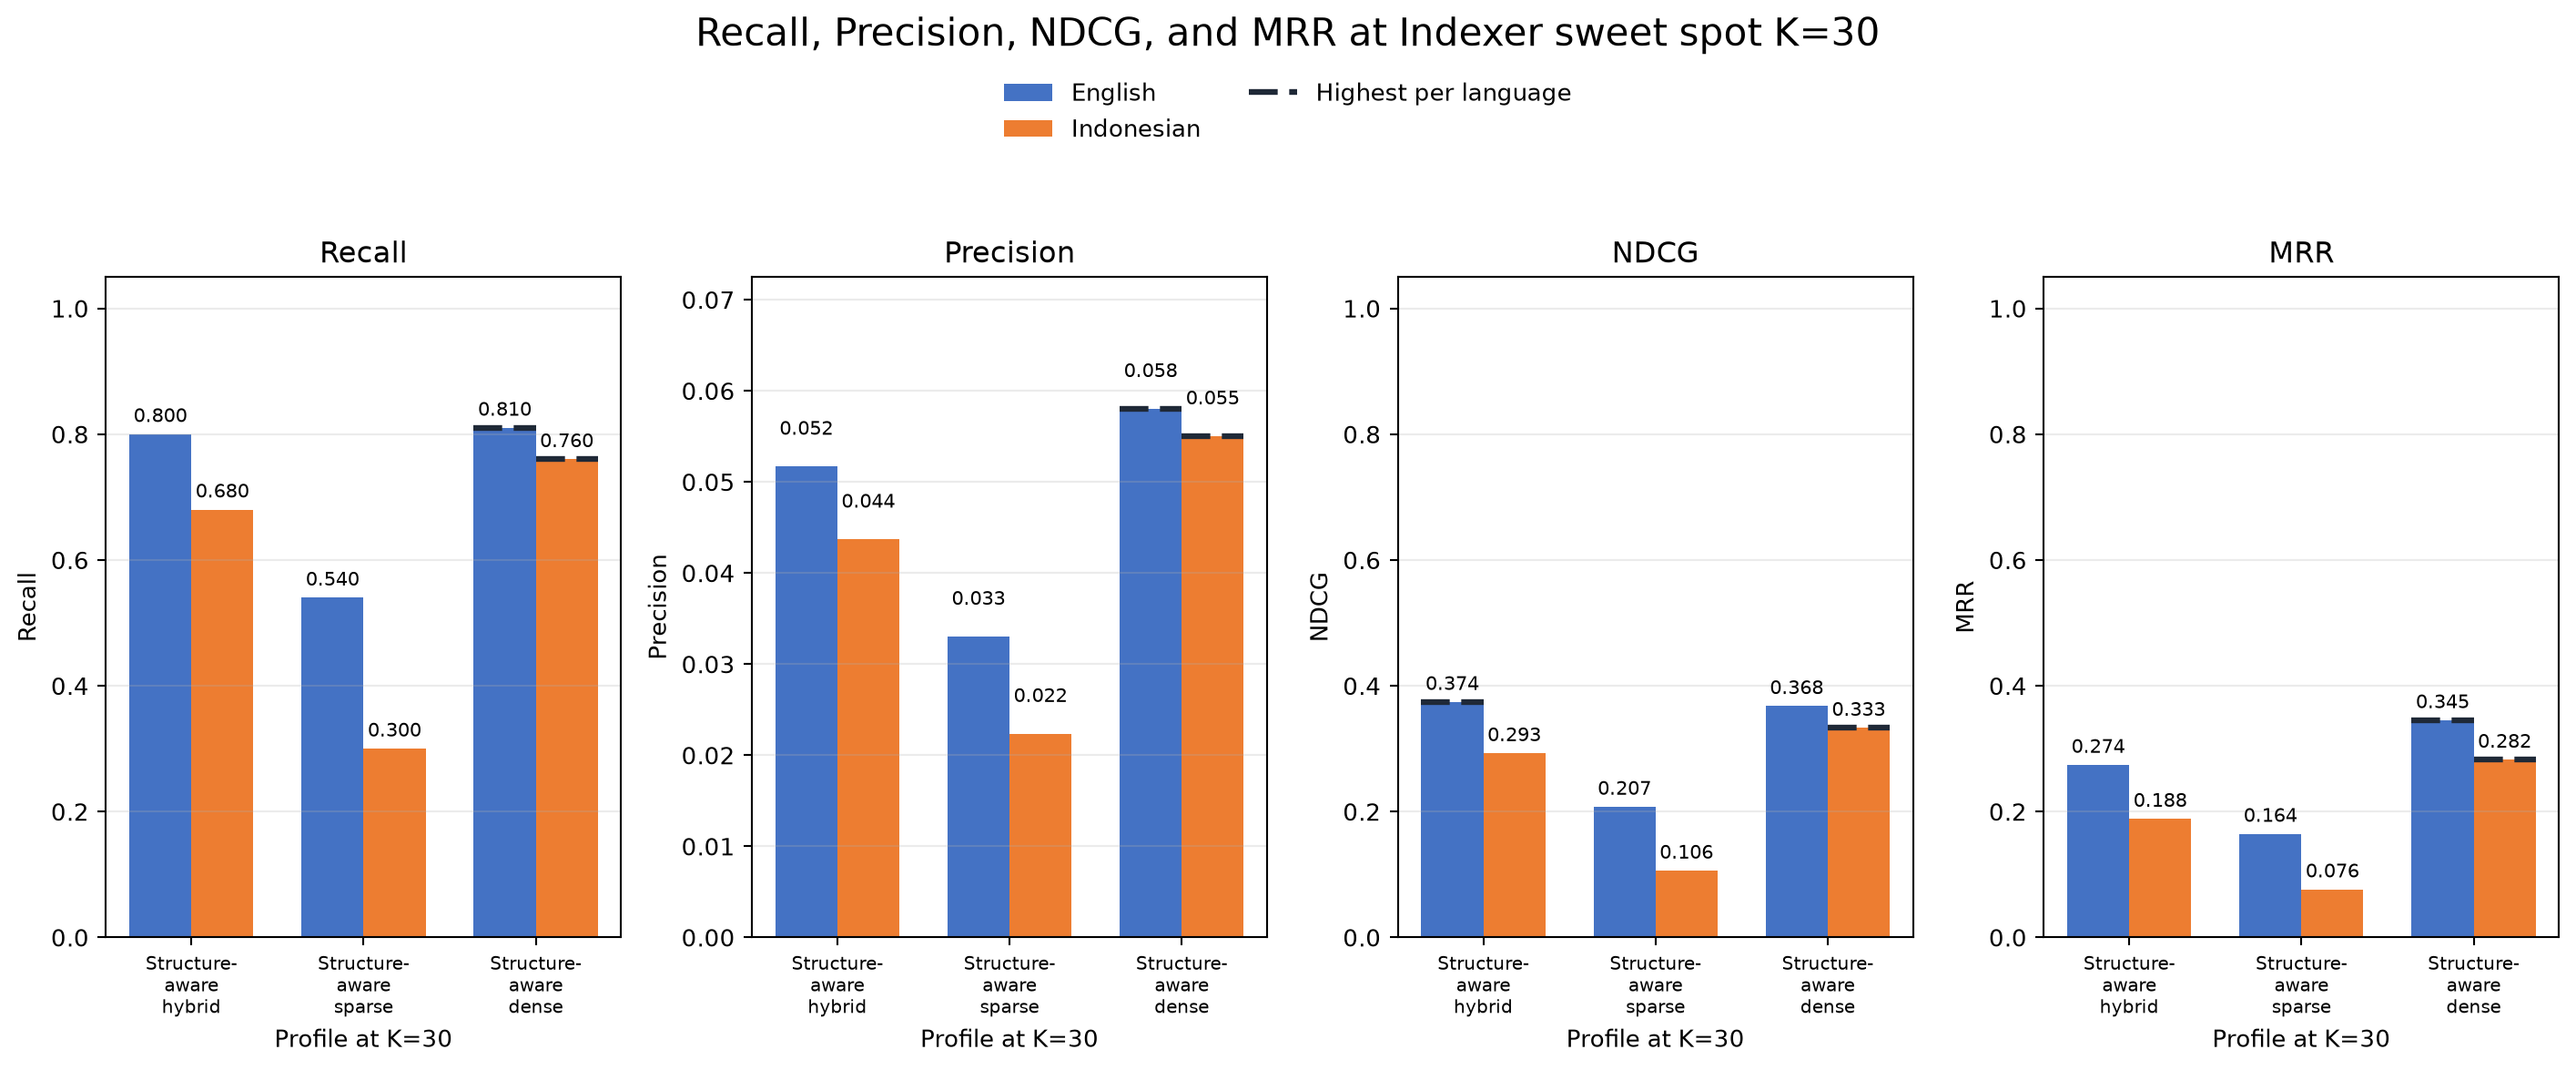
\includegraphics[width=\textwidth,height=0.52\textheight,keepaspectratio]{images/experiments/customer_service_revision/final_eda/metrics-at-sweet-spot-indexer.png}
\caption{\emph{Recall}, \emph{precision}, \emph{NDCG}, dan \emph{MRR} konfigurasi \emph{indexer} pada \(K = 30\)}
\label{fig:customer-indexer-sweet-spot}
\end{figure}

\paragraph{\emph{Generation} pada kelompok \emph{indexer}.}
Dengan \emph{chunker} \emph{structure-aware}, \emph{evidence} \(K = 10\) dari setiap \emph{indexer} dikirim ke \texttt{openai/gpt-5.6-luna}.
\emph{Correctness} menunjukkan seberapa banyak isi
acuan yang dapat dibentuk dari sepuluh konteks tersebut, sedangkan \emph{faithfulness} menunjukkan
apakah klaim yang dibentuk benar-benar bersumber dari konteks yang dikirim. Kedua nilai
dilaporkan terpisah untuk setiap konfigurasi. Estimasi \emph{token} \emph{payload} \emph{generation} adalah sekitar
3.514 untuk \emph{hybrid}, 3.708 untuk \emph{sparse}, dan 3.399 untuk \emph{dense}. Dengan demikian, \emph{dense} tidak
menjadi unggul karena mengirim \emph{evidence} paling banyak. Yang dibandingkan adalah kualitas \emph{evidence}
yang berada pada sepuluh posisi awal.

\begin{figure}[H]
\centering
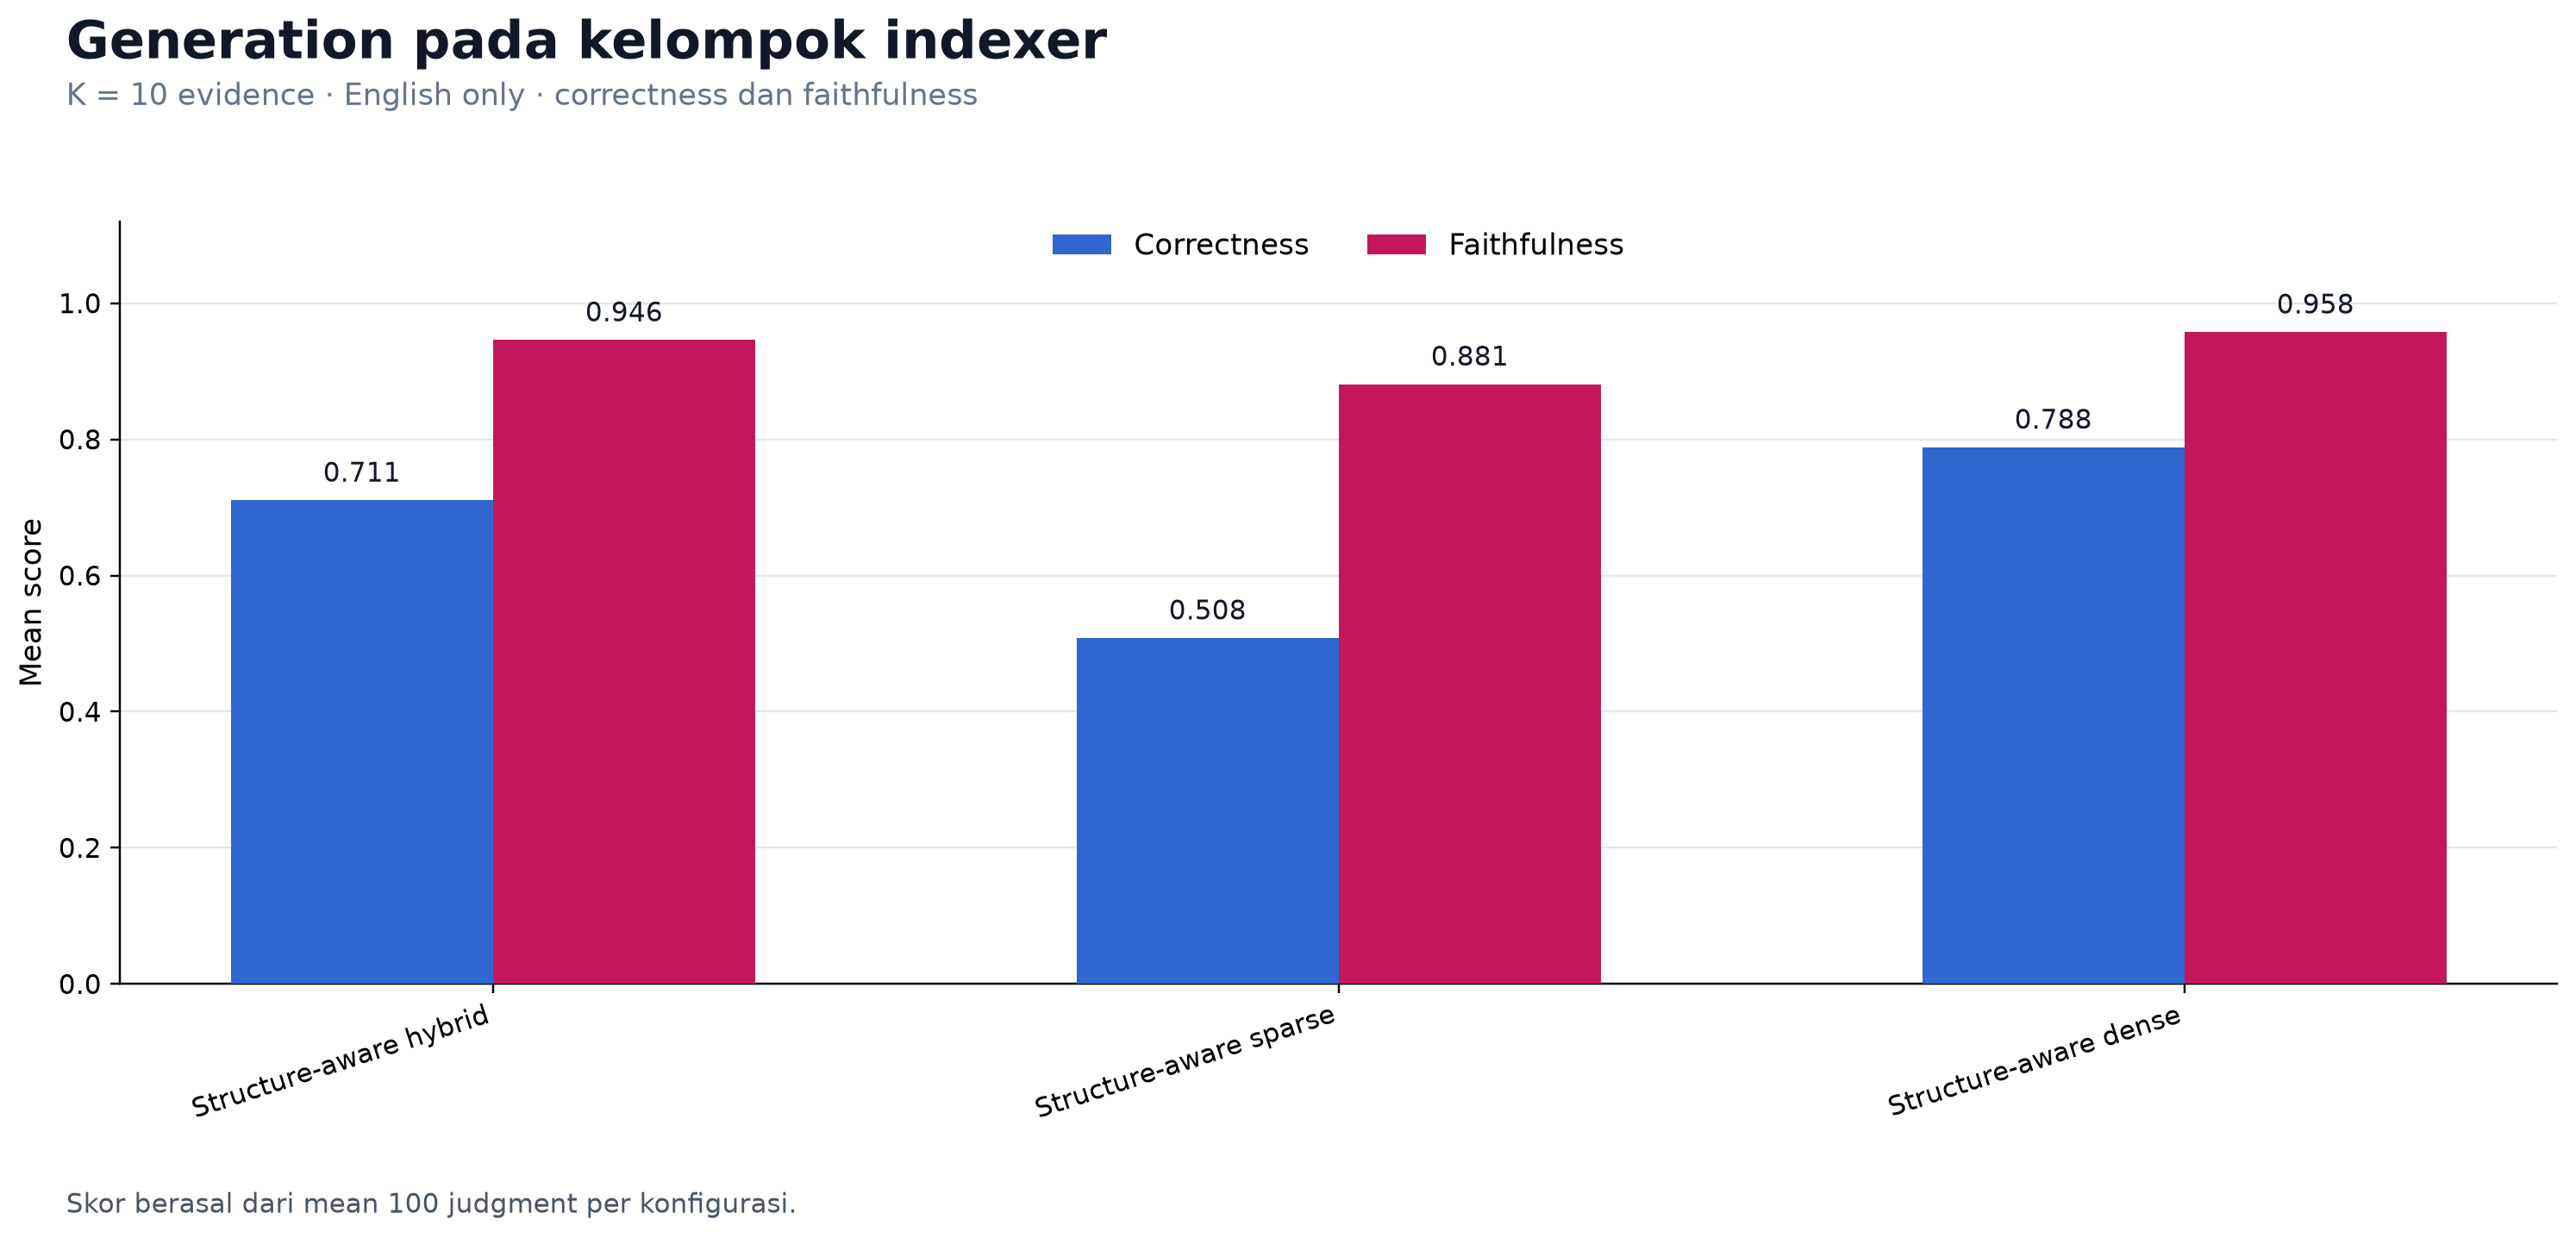
\includegraphics[width=\textwidth,height=0.43\textheight,keepaspectratio]{images/experiments/customer_service_revision/final_eda/generation-indexer.png}
\caption{\emph{Correctness} dan \emph{faithfulness} \emph{generation} pada kelompok \emph{indexer} dengan \(K = 10\)}
\label{fig:customer-indexer-generation-bar}
\end{figure}

Pada Gambar~\ref{fig:customer-indexer-generation-bar}, \emph{structure-aware} \emph{dense} memperoleh
\emph{correctness} 0,788 dan \emph{faithfulness} 0,958, nilai tertinggi pada kelompok \emph{indexer}.
Payload-nya sekitar 3.399 \emph{token}, tetapi \emph{retrieval} \emph{dense} pada \(K = 30\) juga memiliki \emph{recall}
0,785, \emph{NDCG} 0,350, dan \emph{MRR} 0,314. Artinya, \emph{volume} yang lebih kecil tetap dapat menghasilkan
jawaban lebih baik ketika \emph{evidence} yang masuk ke posisi awal lebih relevan dan lebih lengkap.

\emph{Structure-aware} \emph{hybrid} memperoleh \emph{correctness} 0,711 dan \emph{faithfulness} 0,946. Nilai \emph{faithfulness}
yang tetap tinggi menunjukkan bahwa \emph{evidence} yang dikirim cukup mendukung klaim yang ditulis,
tetapi \emph{correctness} lebih rendah karena recall-nya berada di bawah \emph{dense}. \emph{Payload} \emph{hybrid} sekitar
3.514 \emph{token}, hampir sama dengan \emph{dense}, sehingga selisih hasil terutama berkaitan dengan \emph{reference}
yang berhasil ditempatkan pada kandidat awal.

\emph{Structure-aware} \emph{sparse} memperoleh \emph{correctness} 0,508 dan \emph{faithfulness} 0,881 dengan \emph{payload} sekitar
3.708 \emph{token}, paling besar di antara ketiga \emph{indexer}. \emph{Evidence} yang lebih banyak tidak membantu
ketika kecocokan istilahnya lemah. Jawaban lebih sering kekurangan isi acuan dan faithfulness-nya
lebih rendah. Pola ini menegaskan bahwa \emph{volume} \emph{token} harus dibaca bersama \emph{recall} dan kualitas
peringkat, bukan sebagai ukuran kualitas \emph{generation} secara tunggal.

Perbandingan ini menunjukkan bahwa \emph{volume} \emph{evidence} bukan penentu tunggal \emph{generation}. Kualitas
penempatan \emph{reference} pada daftar awal lebih penting. Dengan \emph{chunker} yang sama, perubahan pada
\emph{indexer} terlihat langsung pada kelengkapan jawaban, sehingga \emph{structure-aware} \emph{dense} dipilih
sebagai konfigurasi \emph{indexer} acuan untuk eksperimen sistem.

\subsection{Eksperimen Sistem \emph{Retrieval}}
\label{subsec:user-manual-system-retrieval}

Eksperimen sistem menyatukan lima konfigurasi yang telah dipilih pada eksperimen \emph{chunker} dan
\emph{indexer}, lalu membandingkannya pada \emph{cutoff} bersama \(K = 30\). Tidak ada \emph{chunker} atau \emph{indexer}
baru pada tahap ini. \emph{Recall} tetap menjadi dasar perbandingan, sedangkan \emph{precision}, \emph{MRR}, dan \emph{NDCG}
menjadi metrik pendukung untuk membaca kepadatan dan posisi hasil.

\paragraph{Diagnosis awal pada \(K = 1\).}
Pada \(K = 1\), hanya satu kandidat dengan peringkat tertinggi yang tersedia. Karena setiap
pertanyaan memiliki satu \emph{context reference}, \emph{recall}, \emph{precision}, keberhasilan pertanyaan,
\emph{MRR}, dan \emph{NDCG} pada titik ini sama-sama menunjukkan apakah kandidat pertama tersebut merupakan
hit. Hasil gabungan menunjukkan bahwa \emph{Structure-aware} \emph{dense} mencapai 0,185 (37 dari 200
pertanyaan), \emph{Recursive} dan \emph{Sliding-window} masing-masing 0,120 (24 dari 200), \emph{Structure-aware}
\emph{hybrid} 0,105 (21 dari 200), dan \emph{Structure-aware} \emph{sparse} 0,060 (12 dari 200).

\begin{table}[H]
\centering
\scriptsize
\caption{\emph{Recall} \emph{context reference} pada diagnosis top-1 \emph{User Manual}}
\label{tab:customer-k1-diagnostic}
\begin{tabularx}{\textwidth}{@{}>{\RaggedRight\arraybackslash}Xrrr@{}}
\toprule
\textbf{Konfigurasi} & \textbf{Gabungan} & \textbf{Inggris} & \textbf{Indonesia}\\
\midrule
\emph{Structure-aware dense} & \textbf{0,185} (37/200) & \textbf{0,220} & \textbf{0,150}\\
\emph{Recursive} & 0,120 (24/200) & 0,140 & 0,100\\
\emph{Baseline chunker: Sliding-window} & 0,120 (24/200) & 0,140 & 0,100\\
\emph{Structure-aware hybrid} & 0,105 (21/200) & 0,150 & 0,060\\
\emph{Baseline indexer: Structure-aware sparse} & 0,060 (12/200) & 0,090 & 0,030\\
\bottomrule
\end{tabularx}
\end{table}

Nilai top-1 ini belum layak dijadikan \emph{cutoff} operasional. Jika \emph{context reference} tidak muncul
sebagai kandidat pertama, \emph{reranker} tidak dapat memulihkannya karena \emph{reranker} hanya mengurutkan
ulang kandidat yang sudah tersedia. Tahap \emph{retrieval} karena itu perlu mengirim beberapa kandidat
agar \emph{downstream} memiliki pilihan untuk memperbaiki urutan dan tetap mempertahankan \emph{coverage}.
Kenaikan dari satu kandidat menuju \(K = 30\) menaikkan \emph{recall} gabungan menjadi 0,625--0,785
bergantung pada konfigurasi, sehingga \(K = 30\) lebih sesuai sebagai \emph{cutoff} kandidat untuk
\emph{reranker}. \(K = 1\) dipertahankan sebagai diagnosis kemampuan pilihan pertama, bukan sebagai
pengganti proses \emph{candidate} \emph{generation}.

Daftar hasil pada \(K = 30\) merupakan \emph{payload} kandidat untuk tahap \emph{downstream}, yaitu \emph{reranker},
bukan \emph{payload} yang langsung diberikan kepada \emph{generation}. Ukuran \emph{payload} dihitung dari hasil pencatatan
\emph{retrieval}, terdiri atas 100 pertanyaan Inggris dan 100 pertanyaan Indonesia. Estimasi \emph{token}
menggunakan panjang teks kandidat dibagi empat. Tabel~\ref{tab:customer-system-volume} hanya
merangkum panjang \emph{payload} dalam karakter, kata, estimasi \emph{token}, dan persentil ke-95 \emph{token}.

\begin{table}[H]
\centering
\scriptsize
\caption{Ukuran \emph{payload} kandidat untuk \emph{reranker} pada \(K = 30\)}
\label{tab:customer-system-volume}
\begin{tabularx}{\textwidth}{@{}>{\RaggedRight\arraybackslash}p{4.0cm}rrrr@{}}
\toprule
\textbf{Konfigurasi} & \textbf{Karakter} & \textbf{Kata} & \textbf{\emph{Token} est.} & \textbf{P95 \emph{token}}\\
\midrule
\emph{Structure-aware hybrid} & 10.150 & 1.707 & 2.538 & 3.525\\
\emph{Recursive} & 10.099 & 1.693 & 2.525 & 3.579\\
\emph{Sliding-window} & 12.477 & 2.104 & 3.119 & 3.852\\
\emph{Structure-aware sparse} & 10.941 & 1.848 & 2.735 & 3.590\\
\emph{Structure-aware dense} & 13.238 & 2.219 & 3.309 & 3.597\\
\bottomrule
\end{tabularx}
\end{table}

Nilai karakter, kata, dan estimasi \emph{token} pada tabel merupakan nilai rerata \emph{payload} per pertanyaan,
sedangkan P95 menunjukkan batas 95 persen \emph{payload} terpanjang. \emph{Sliding-window} membawa \emph{payload}
terbesar, sementara \emph{hybrid} dan \emph{recursive} lebih ringkas. Ukuran ini digunakan untuk memperkirakan
beban \emph{reranker}. \emph{Generation} tetap memakai \(K = 10\) dan diukur terpisah pada bagian \emph{generation},
sehingga angka pada tabel ini tidak boleh dibaca sebagai \emph{volume} konteks \emph{generation}.

\begin{figure}[H]
\centering
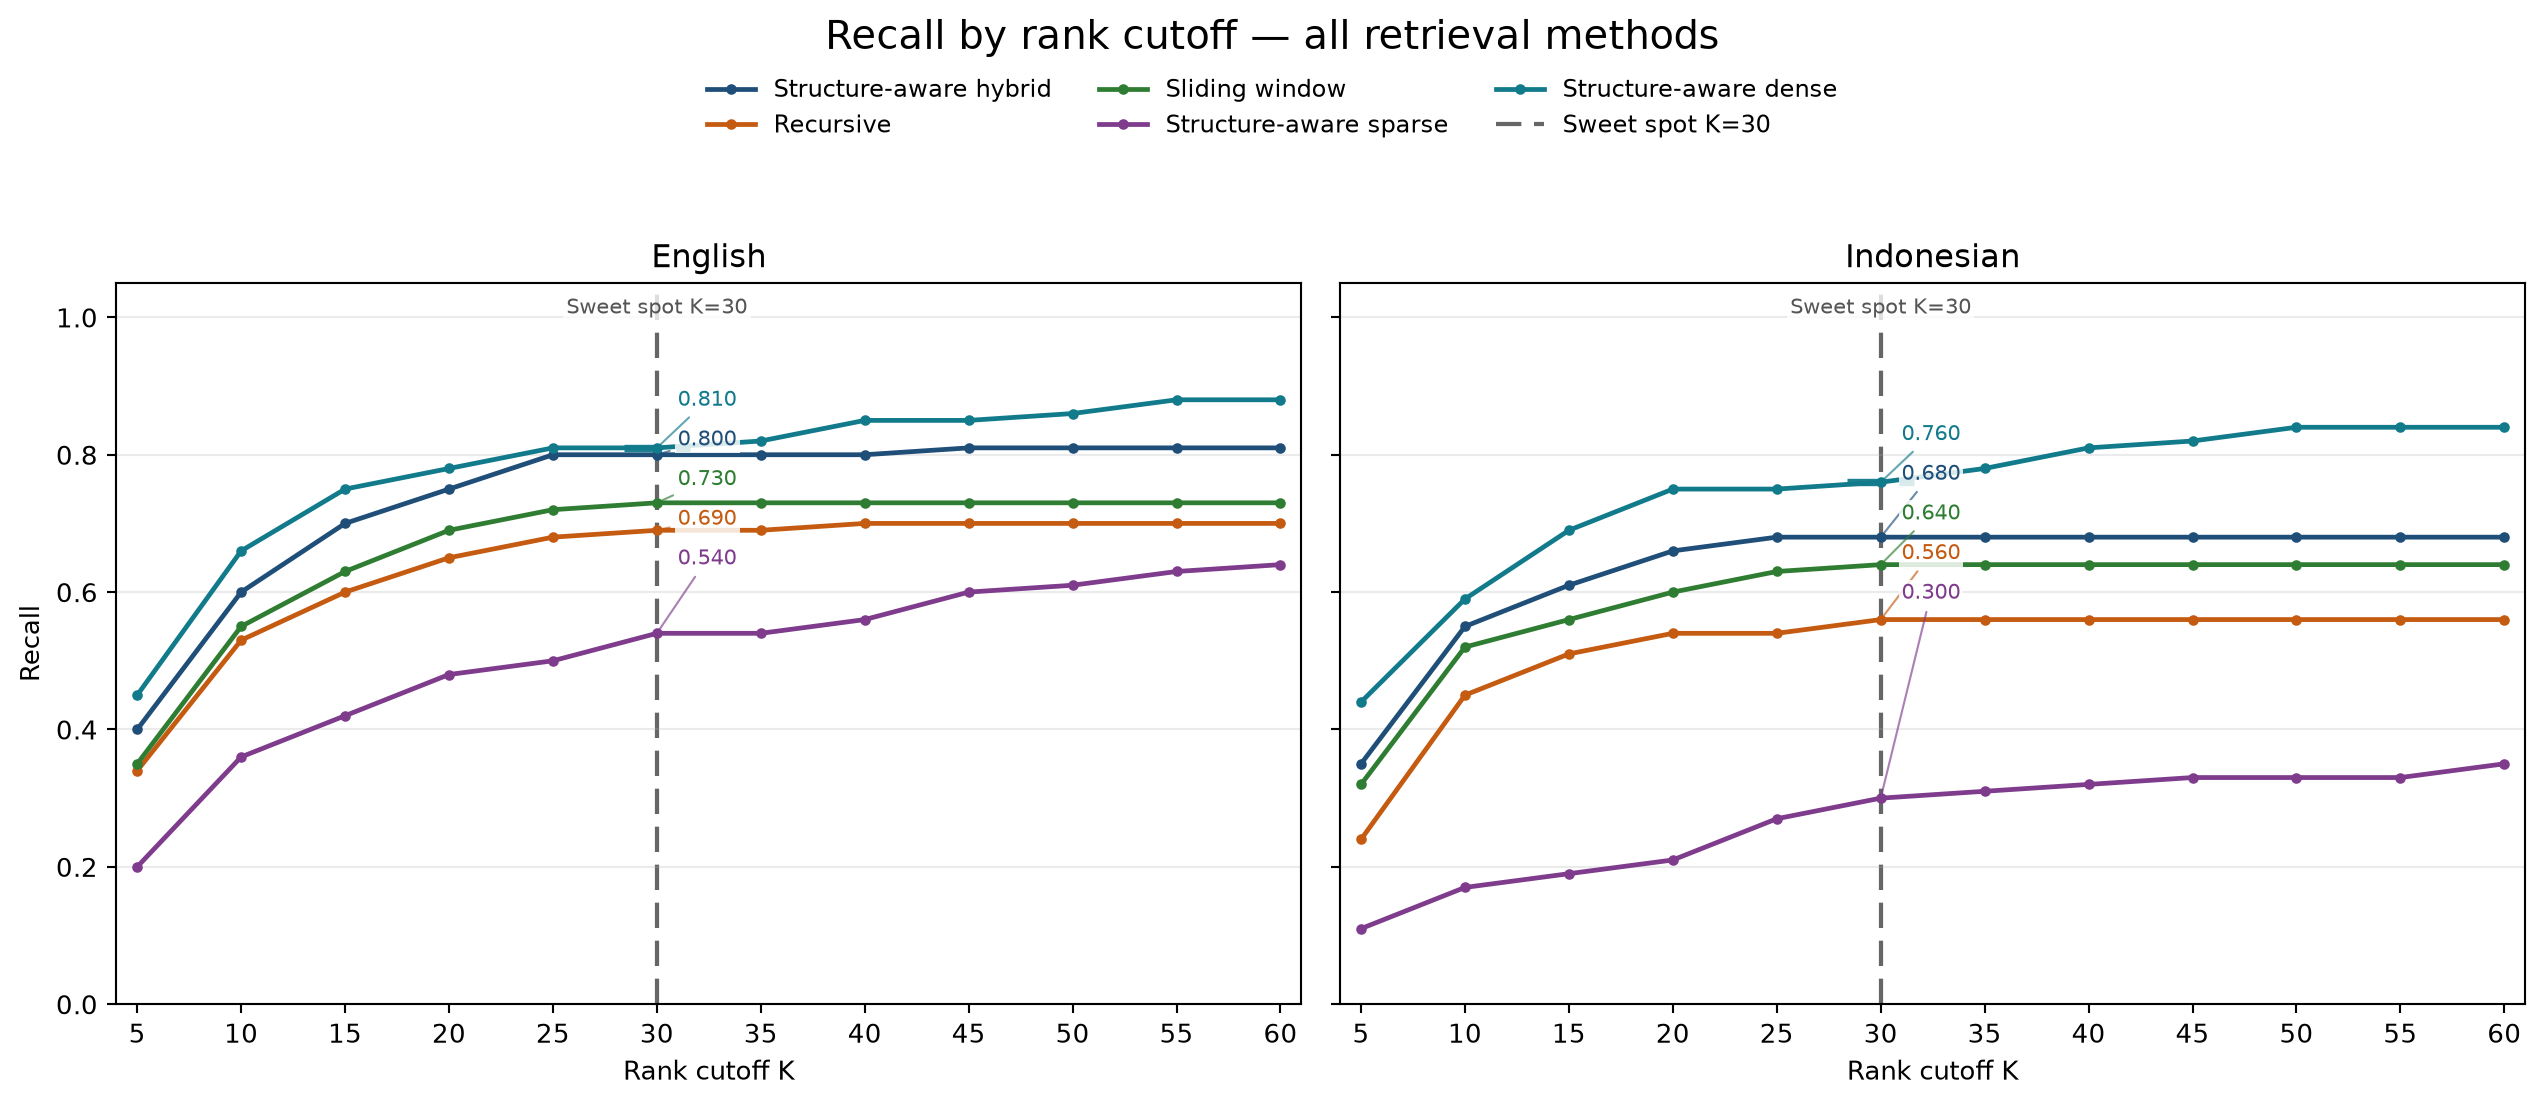
\includegraphics[width=\textwidth,height=0.52\textheight,keepaspectratio]{images/experiments/customer_service_revision/final_eda/recall-all-retrieval.png}
\caption{Kurva \emph{context reference} \emph{recall} untuk seluruh metode \emph{retrieval}}
\label{fig:customer-system-recall}
\end{figure}

Gambar~\ref{fig:customer-system-recall} merangkum pola pada dua eksperimen komponen. Pada
\(K = 30\), \emph{structure-aware} \emph{dense} memperoleh \emph{recall} tertinggi, yaitu 0,785, diikuti \emph{hybrid}
0,740, \emph{sliding-window} 0,685, \emph{recursive} 0,625, dan \emph{sparse} 0,420. Urutan ini konsisten dengan
analisis segmentasi dan pencarian pada bagian sebelumnya, termasuk pada panel Inggris dan
Indonesia.

\begin{figure}[H]
\centering
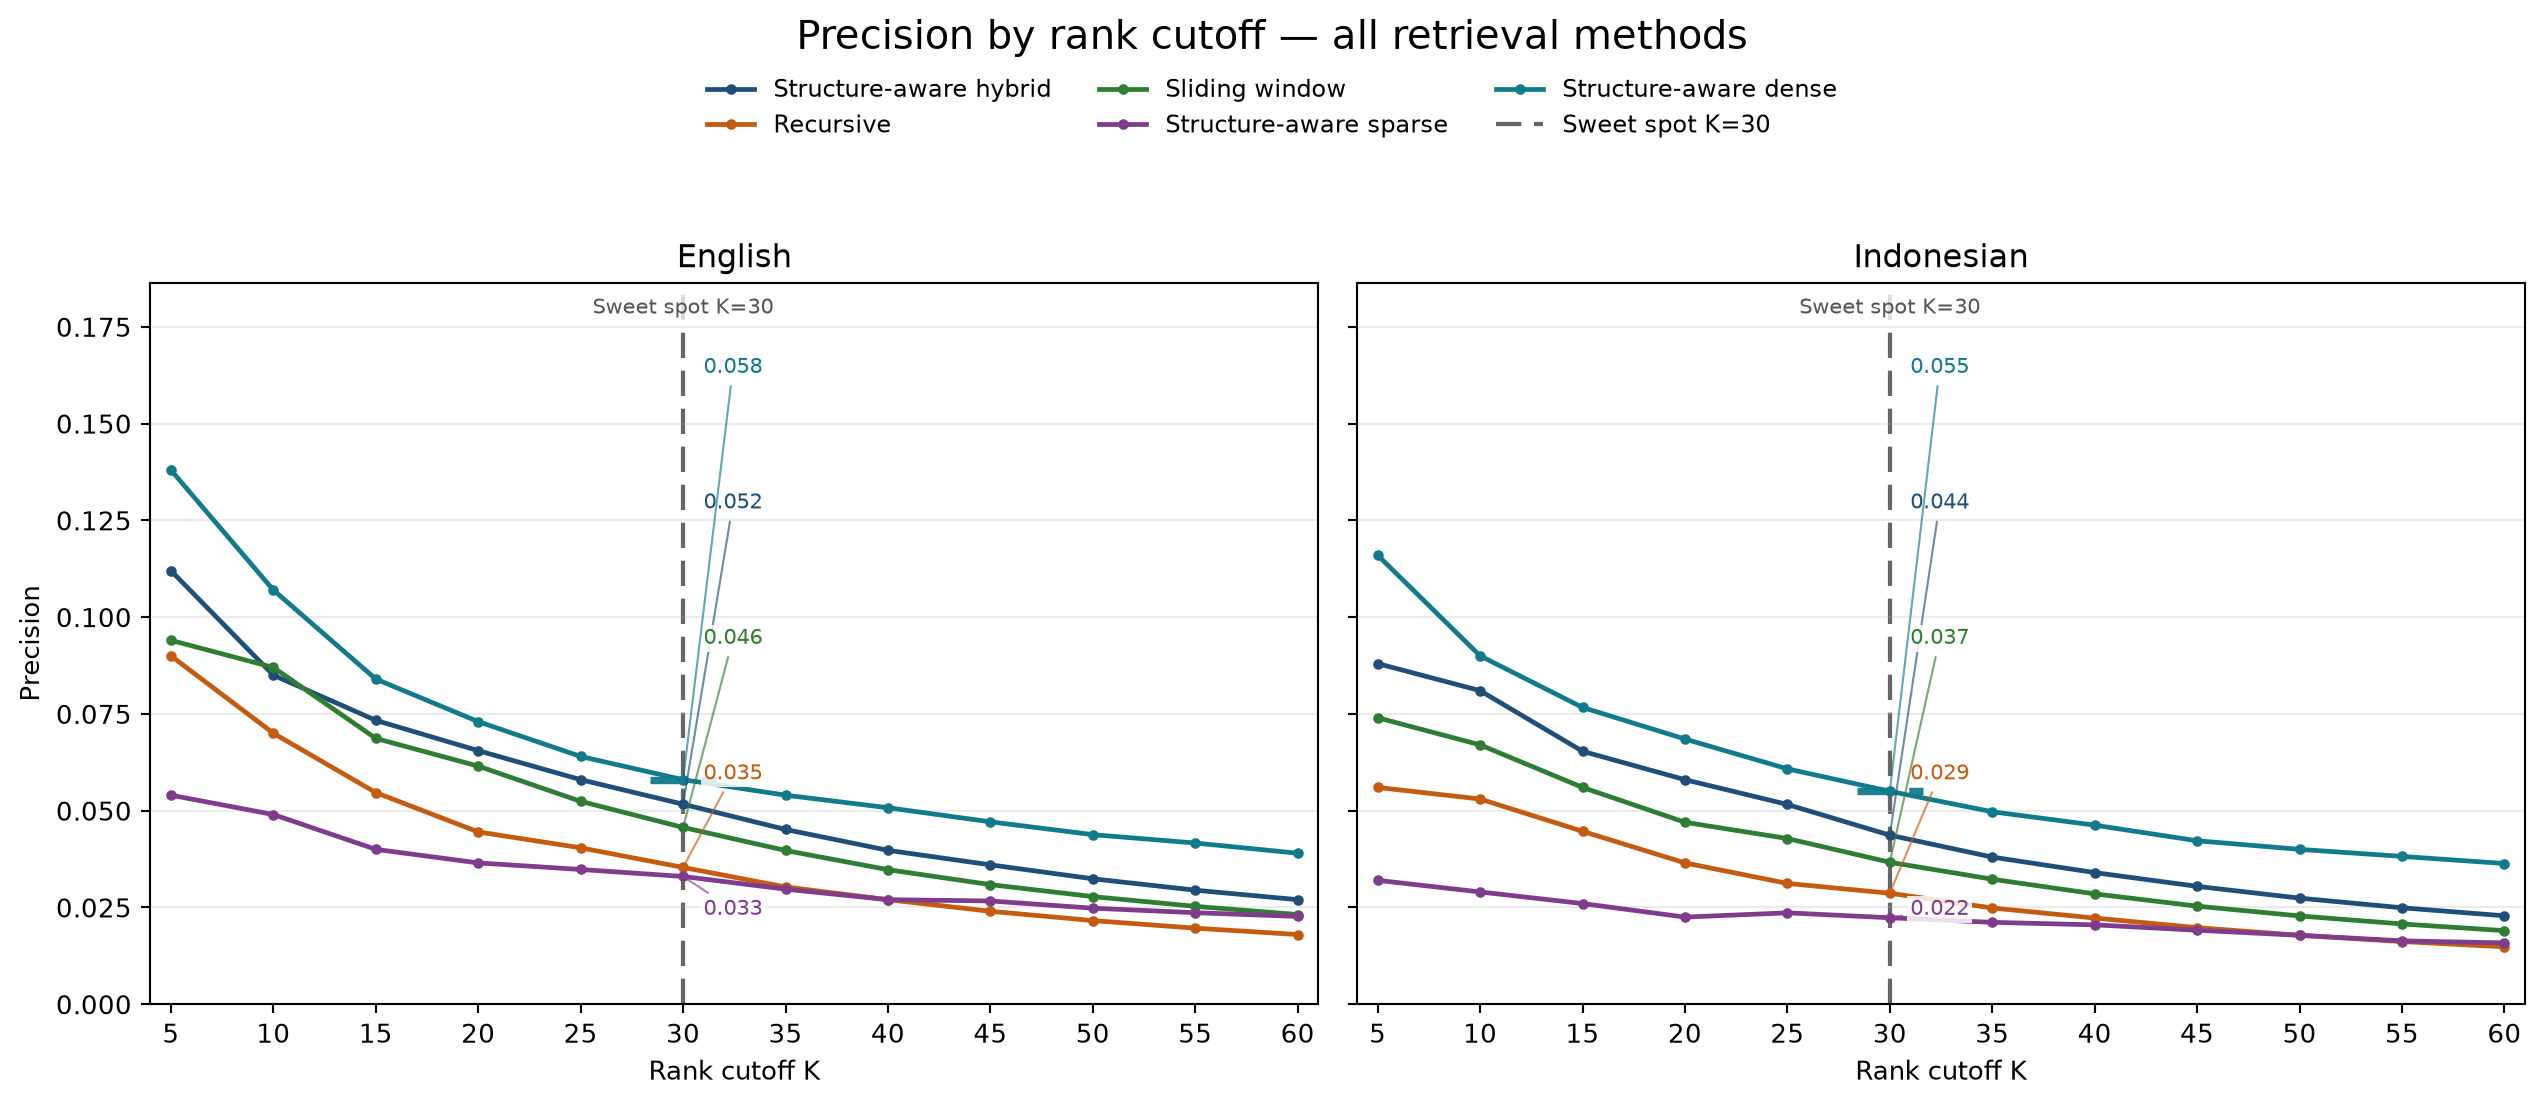
\includegraphics[width=\textwidth,height=0.52\textheight,keepaspectratio]{images/experiments/customer_service_revision/final_eda/precision-all-retrieval.png}
\caption{Kurva \emph{context reference} \emph{precision} untuk seluruh metode \emph{retrieval}}
\label{fig:customer-system-precision}
\end{figure}

Gambar~\ref{fig:customer-system-precision} mengulang kecenderungan \emph{precision} yang menurun
ketika \emph{cutoff} diperbesar. Pada \(K = 30\), \emph{dense} berada di posisi tertinggi dengan 0,057,
diikuti \emph{hybrid} 0,048, \emph{sliding-window} 0,041, \emph{recursive} 0,032, dan \emph{sparse} 0,028. Nilai ini
menjadi rekap kepadatan hasil yang telah dianalisis pada masing-masing komponen.

\begin{figure}[H]
\centering
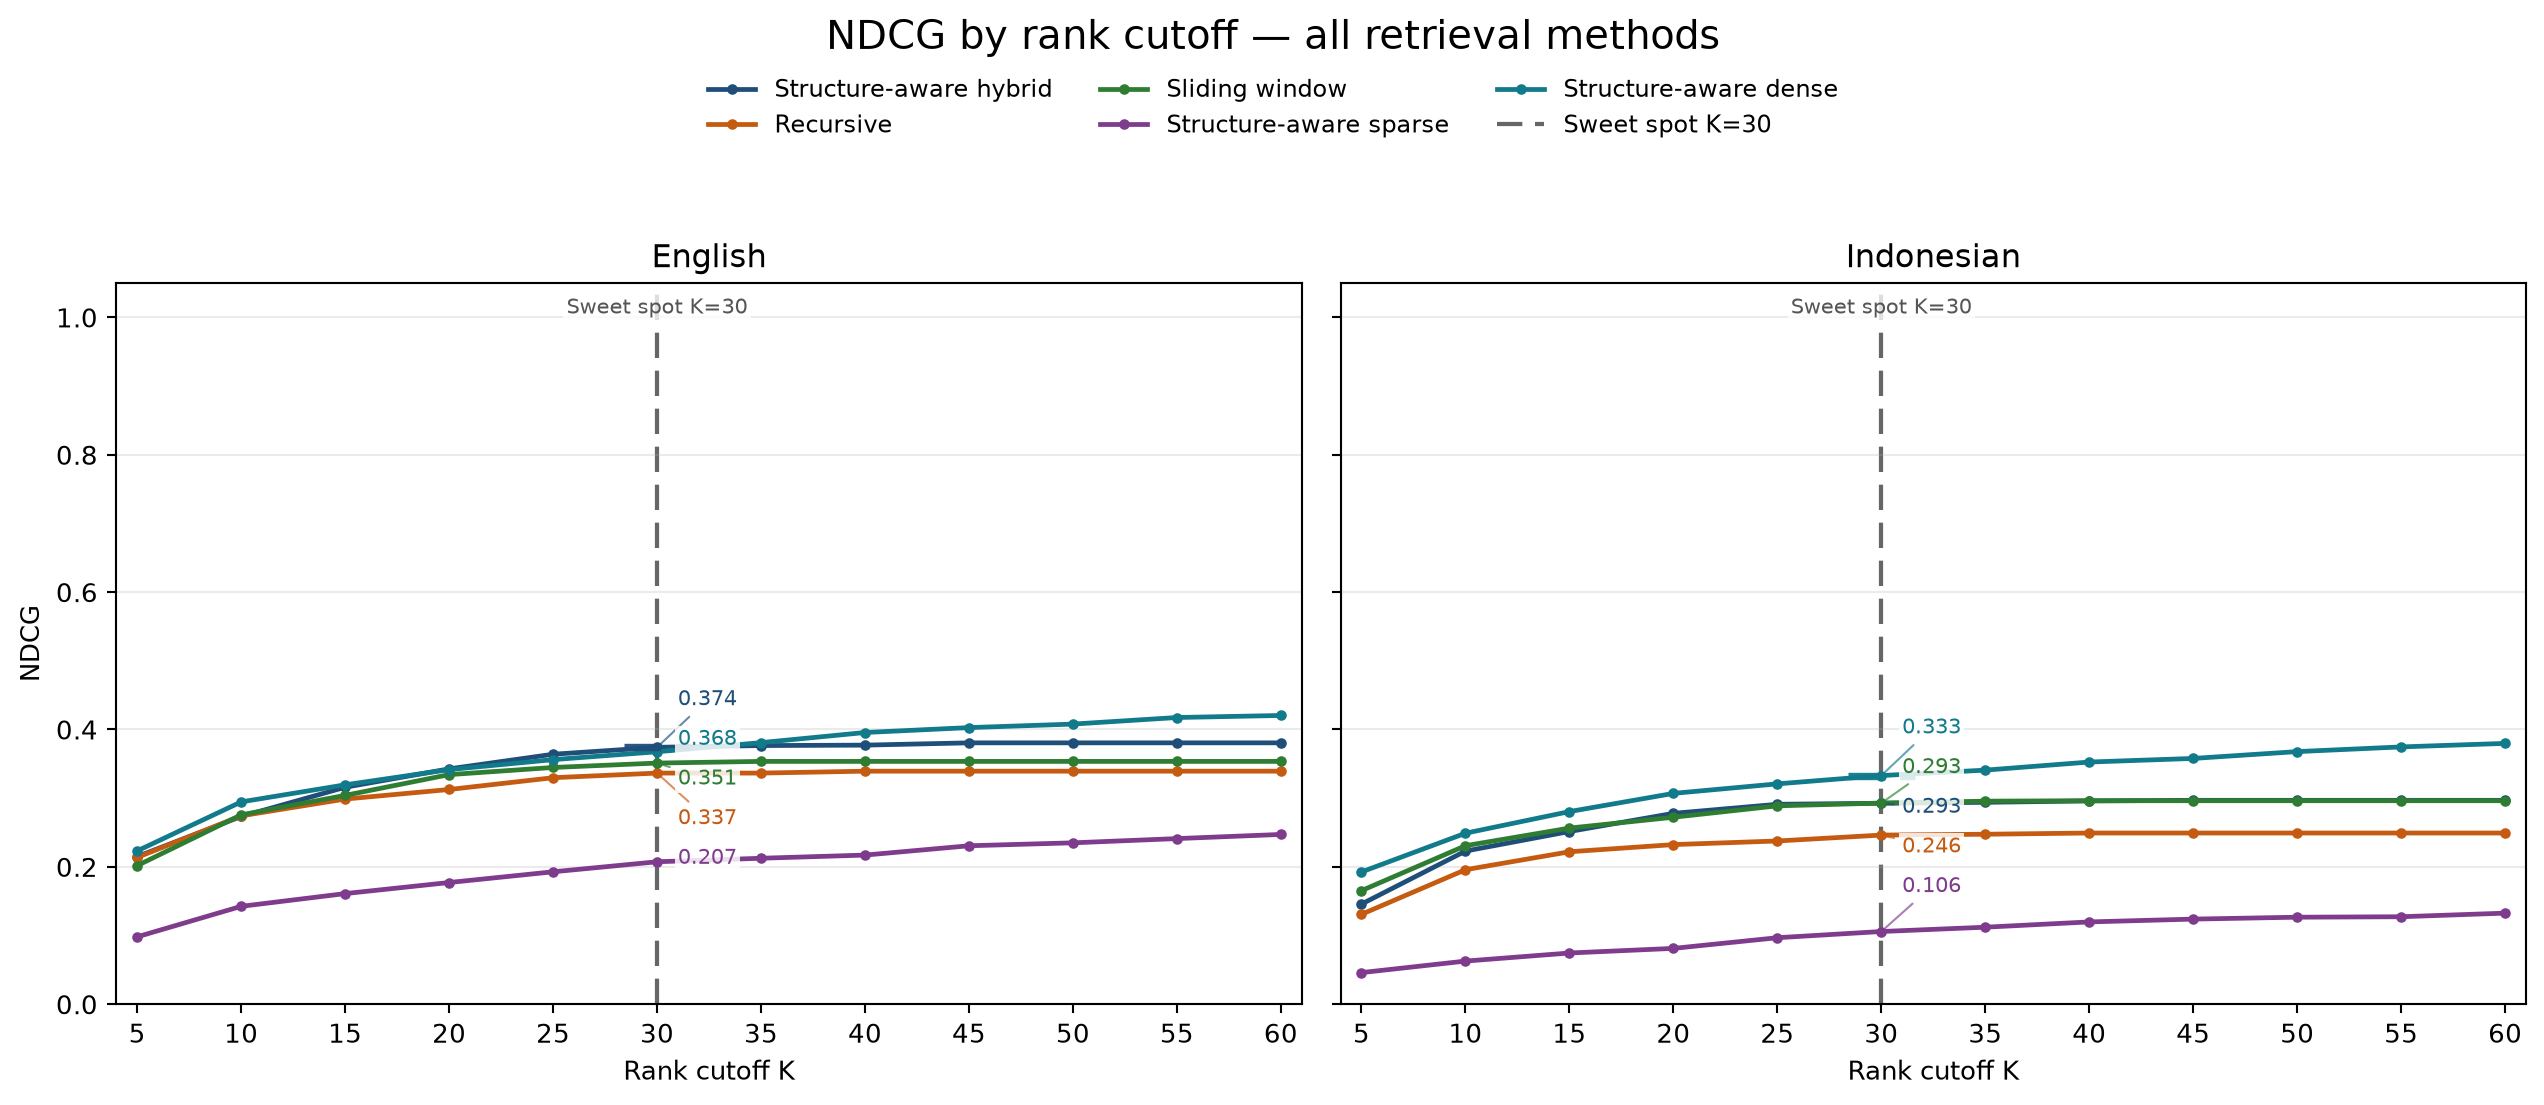
\includegraphics[width=\textwidth,height=0.52\textheight,keepaspectratio]{images/experiments/customer_service_revision/final_eda/ndcg-all-retrieval.png}
\caption{Kurva \emph{NDCG} untuk seluruh metode \emph{retrieval}}
\label{fig:customer-system-ndcg}
\end{figure}

Gambar~\ref{fig:customer-system-ndcg} merangkum \emph{NDCG} pada \(K = 30\), yaitu 0,350 untuk
\emph{dense}, 0,333 untuk \emph{hybrid}, 0,322 untuk \emph{sliding-window}, 0,291 untuk \emph{recursive}, dan 0,157 untuk
\emph{sparse}. Urutan ini sejalan dengan temuan per komponen bahwa \emph{dense} dan \emph{hybrid} menempatkan
\emph{reference} lebih baik daripada konfigurasi lainnya.

\begin{figure}[H]
\centering
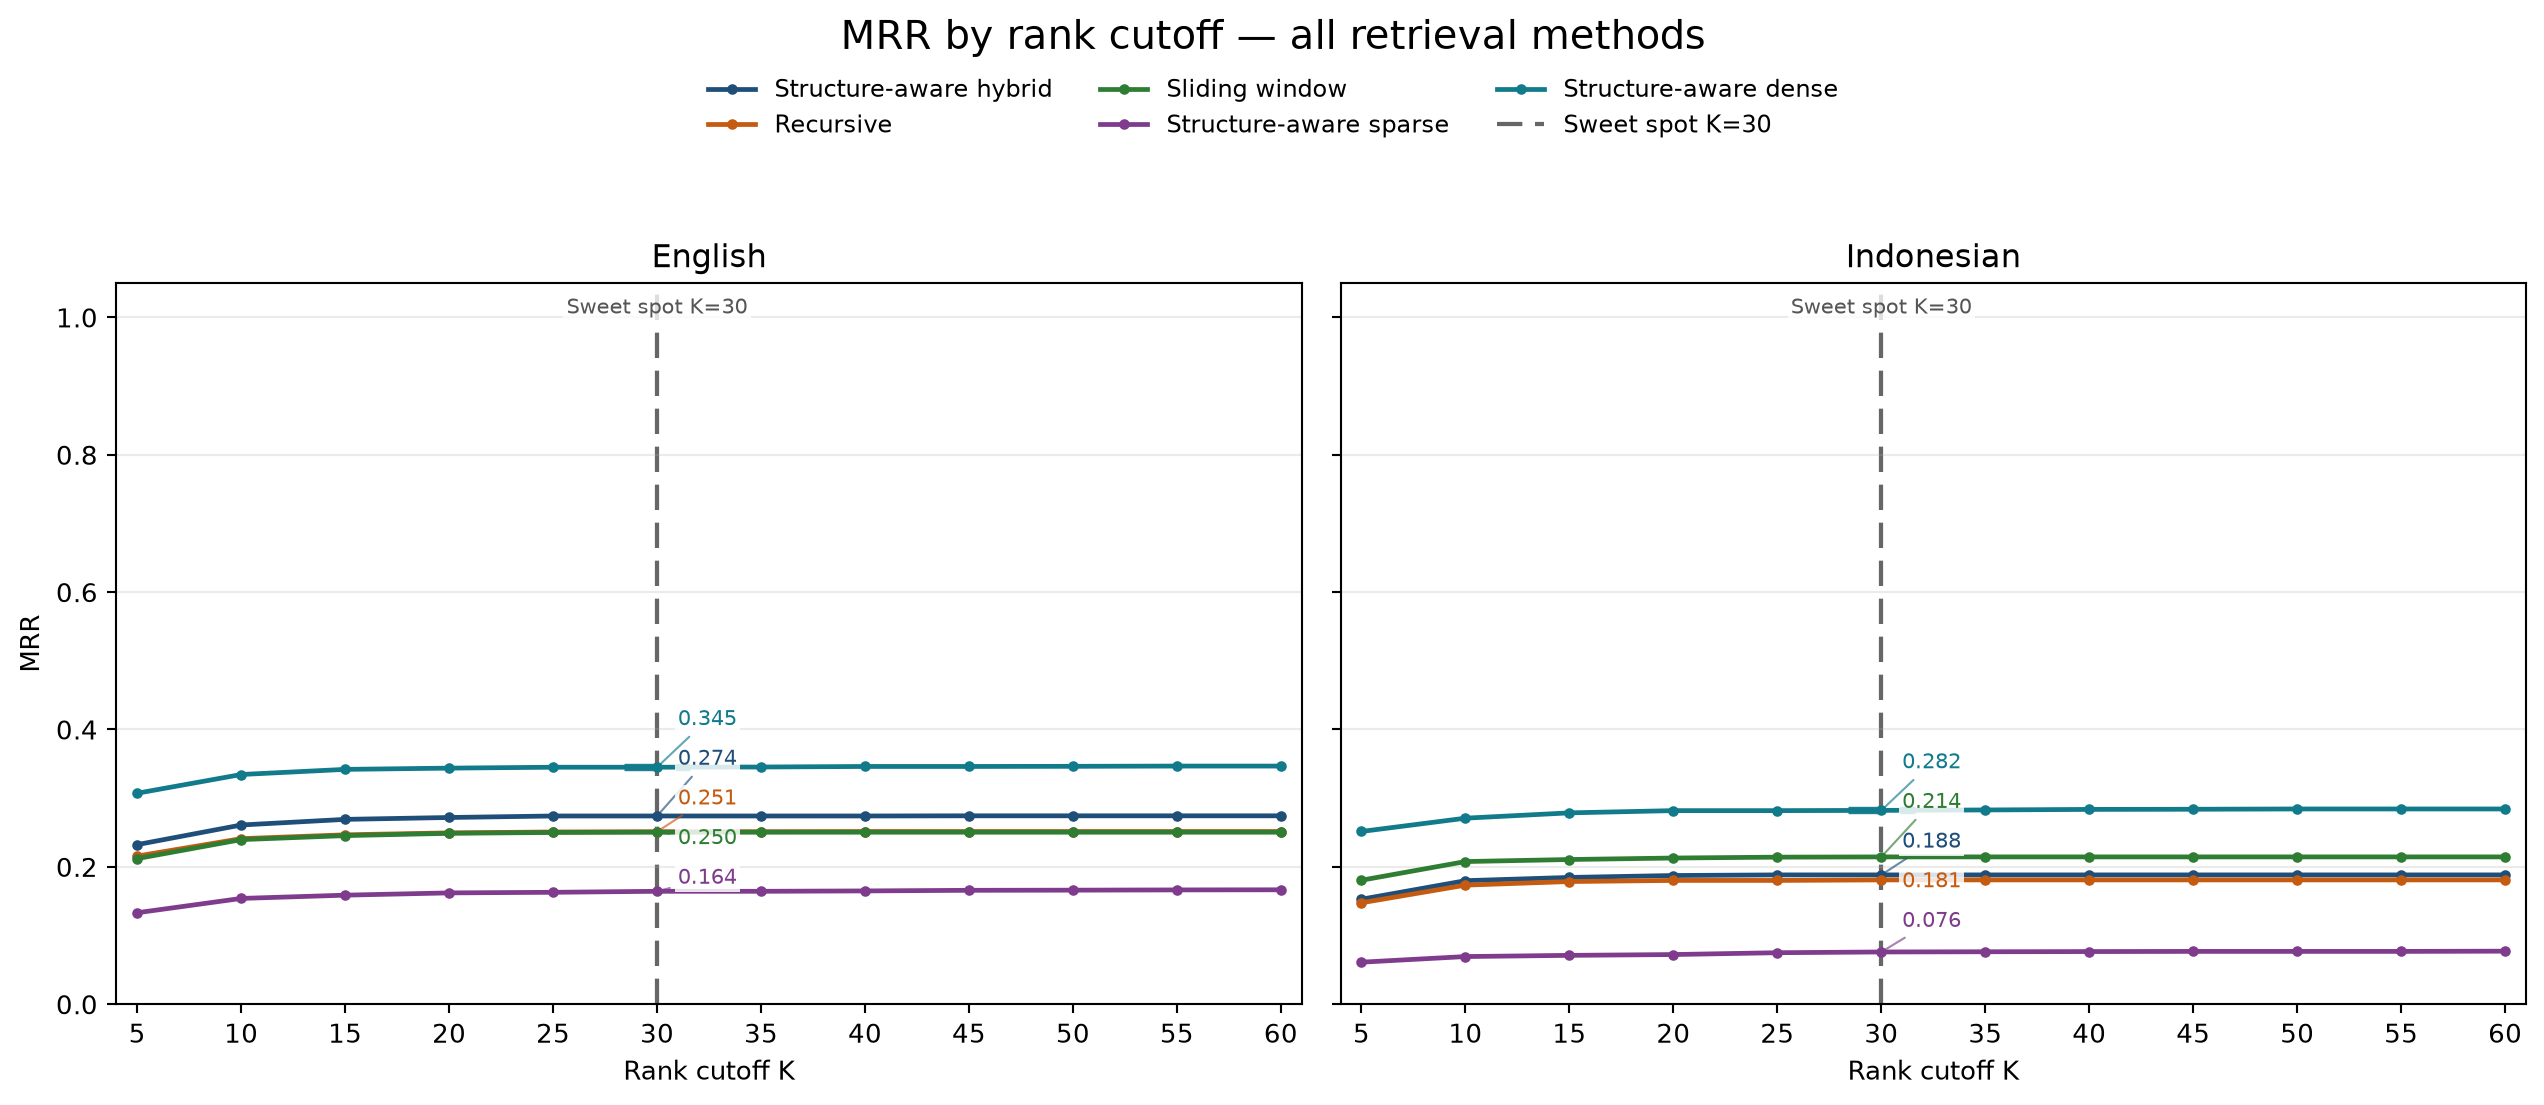
\includegraphics[width=\textwidth,height=0.52\textheight,keepaspectratio]{images/experiments/customer_service_revision/final_eda/mrr-all-retrieval.png}
\caption{Kurva \emph{MRR} untuk seluruh metode \emph{retrieval}}
\label{fig:customer-system-mrr}
\end{figure}

Pada Gambar~\ref{fig:customer-system-mrr}, \emph{MRR} pada \(K = 30\) adalah 0,314 untuk \emph{dense},
0,231 untuk \emph{hybrid}, 0,232 untuk \emph{sliding-window}, 0,216 untuk \emph{recursive}, dan 0,120 untuk \emph{sparse}.
\emph{Dense} tetap paling awal pada hit pertama, sedangkan keunggulan tipis \emph{sliding} atas \emph{hybrid} hanya
merupakan pola posisi hasil dan tidak mengubah keputusan berbasis \emph{recall}.

\begin{table}[H]
\centering
\scriptsize
\caption{Hasil eksperimen sistem \emph{retrieval} \emph{User Manual} pada \emph{sweet spot} bersama}
\label{tab:customer-system-results}
\begin{tabularx}{\textwidth}{@{}>{\RaggedRight\arraybackslash}p{3.7cm} r r r r r@{}}
\toprule
\textbf{Konfigurasi} & \textbf{K} & \textbf{\emph{Recall}} & \textbf{\emph{Precision}} & \textbf{\emph{NDCG}} & \textbf{\emph{MRR}}\\
\midrule
\emph{Structure-aware hybrid} & 30 & 0,740 & 0,048 & 0,333 & 0,231\\
\emph{Recursive} \emph{chunker} & 30 & 0,625 & 0,032 & 0,291 & 0,216\\
\emph{Baseline chunker: Sliding-window} & 30 & 0,685 & 0,041 & 0,322 & 0,232\\
\emph{Baseline indexer: Structure-aware sparse} & 30 & 0,420 & 0,028 & 0,157 & 0,120\\
\emph{Structure-aware dense} & 30 & \textbf{0,785} & \textbf{0,057} & \textbf{0,350} & \textbf{0,314}\\
\bottomrule
\end{tabularx}
\end{table}

Tabel~\ref{tab:customer-system-results} dan Gambar~\ref{fig:customer-system-sweet-spot}
merupakan rekap akhir dari analisis \emph{chunker} dan \emph{indexer}. \emph{Sliding-window} adalah \emph{baseline}
\emph{chunker}, sedangkan \emph{Structure-aware} \emph{sparse} adalah \emph{baseline} \emph{indexer}. \emph{Structure-aware} \emph{hybrid}
mengalahkan \emph{baseline} \emph{chunker} dengan \emph{recall} 0,740 berbanding 0,685, atau delta +0,055.
Pada sisi \emph{indexer}, \emph{Structure-aware} \emph{dense} mengalahkan \emph{baseline} \emph{sparse} dengan \emph{recall} 0,785
berbanding 0,420, atau delta +0,365, dan \emph{Structure-aware} \emph{hybrid} juga mengunggulinya dengan
\emph{recall} 0,740, atau delta +0,320. \emph{Dense} menjadi konfigurasi tertinggi secara keseluruhan,
sementara \emph{hybrid} menjadi strategi \emph{chunker} terbaik. Setiap konfigurasi dihitung secara terpisah
tanpa penggabungan hasil lintas konfigurasi.

\begin{figure}[H]
\centering
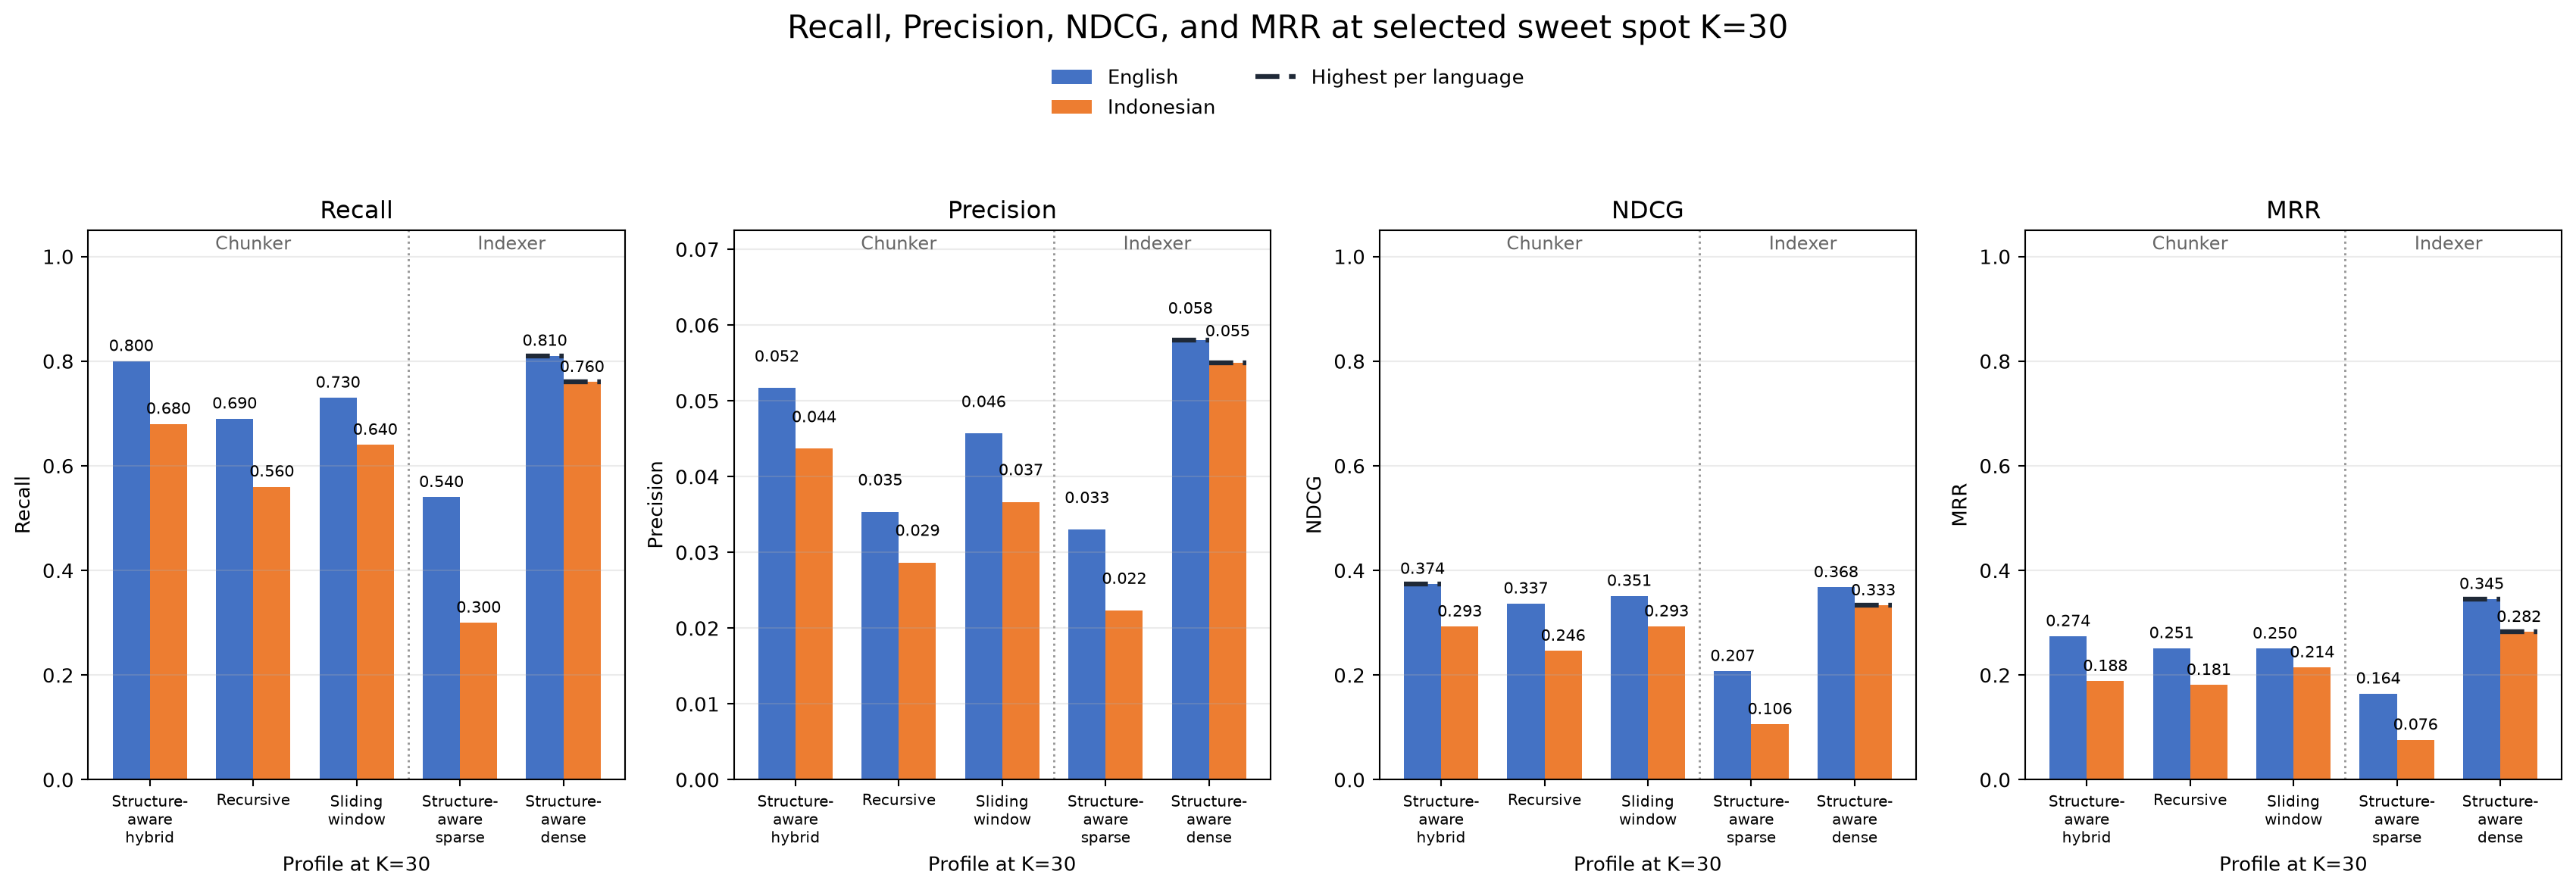
\includegraphics[width=\textwidth,height=0.52\textheight,keepaspectratio]{images/experiments/customer_service_revision/final_eda/metrics-at-sweet-spot.png}
\caption{Ringkasan \emph{recall}, \emph{precision}, \emph{NDCG}, dan \emph{MRR} seluruh konfigurasi pada \(K = 30\)}
\label{fig:customer-system-sweet-spot}
\end{figure}

\subsection{Eksperimen \emph{Generation}}
\label{subsec:user-manual-generation}

Eksperimen \emph{generation} sistem menggunakan konfigurasi yang sama dengan eksperimen \emph{chunker} dan
\emph{indexer}, 100 pertanyaan Inggris, \(K = 10\), \texttt{openai/gpt-5.6-luna}, dan \emph{framework} \emph{Ragas}. Tahap ini
tidak membentuk konfigurasi baru, tetapi menyatukan hasil \emph{generation} dari lima konfigurasi untuk
melihat dampak \emph{retrieval} terhadap jawaban. \emph{Correctness} dan \emph{faithfulness} dihitung terpisah setelah
setiap konfigurasi memiliki 100 jawaban dan penilaian.

\begin{figure}[H]
\centering
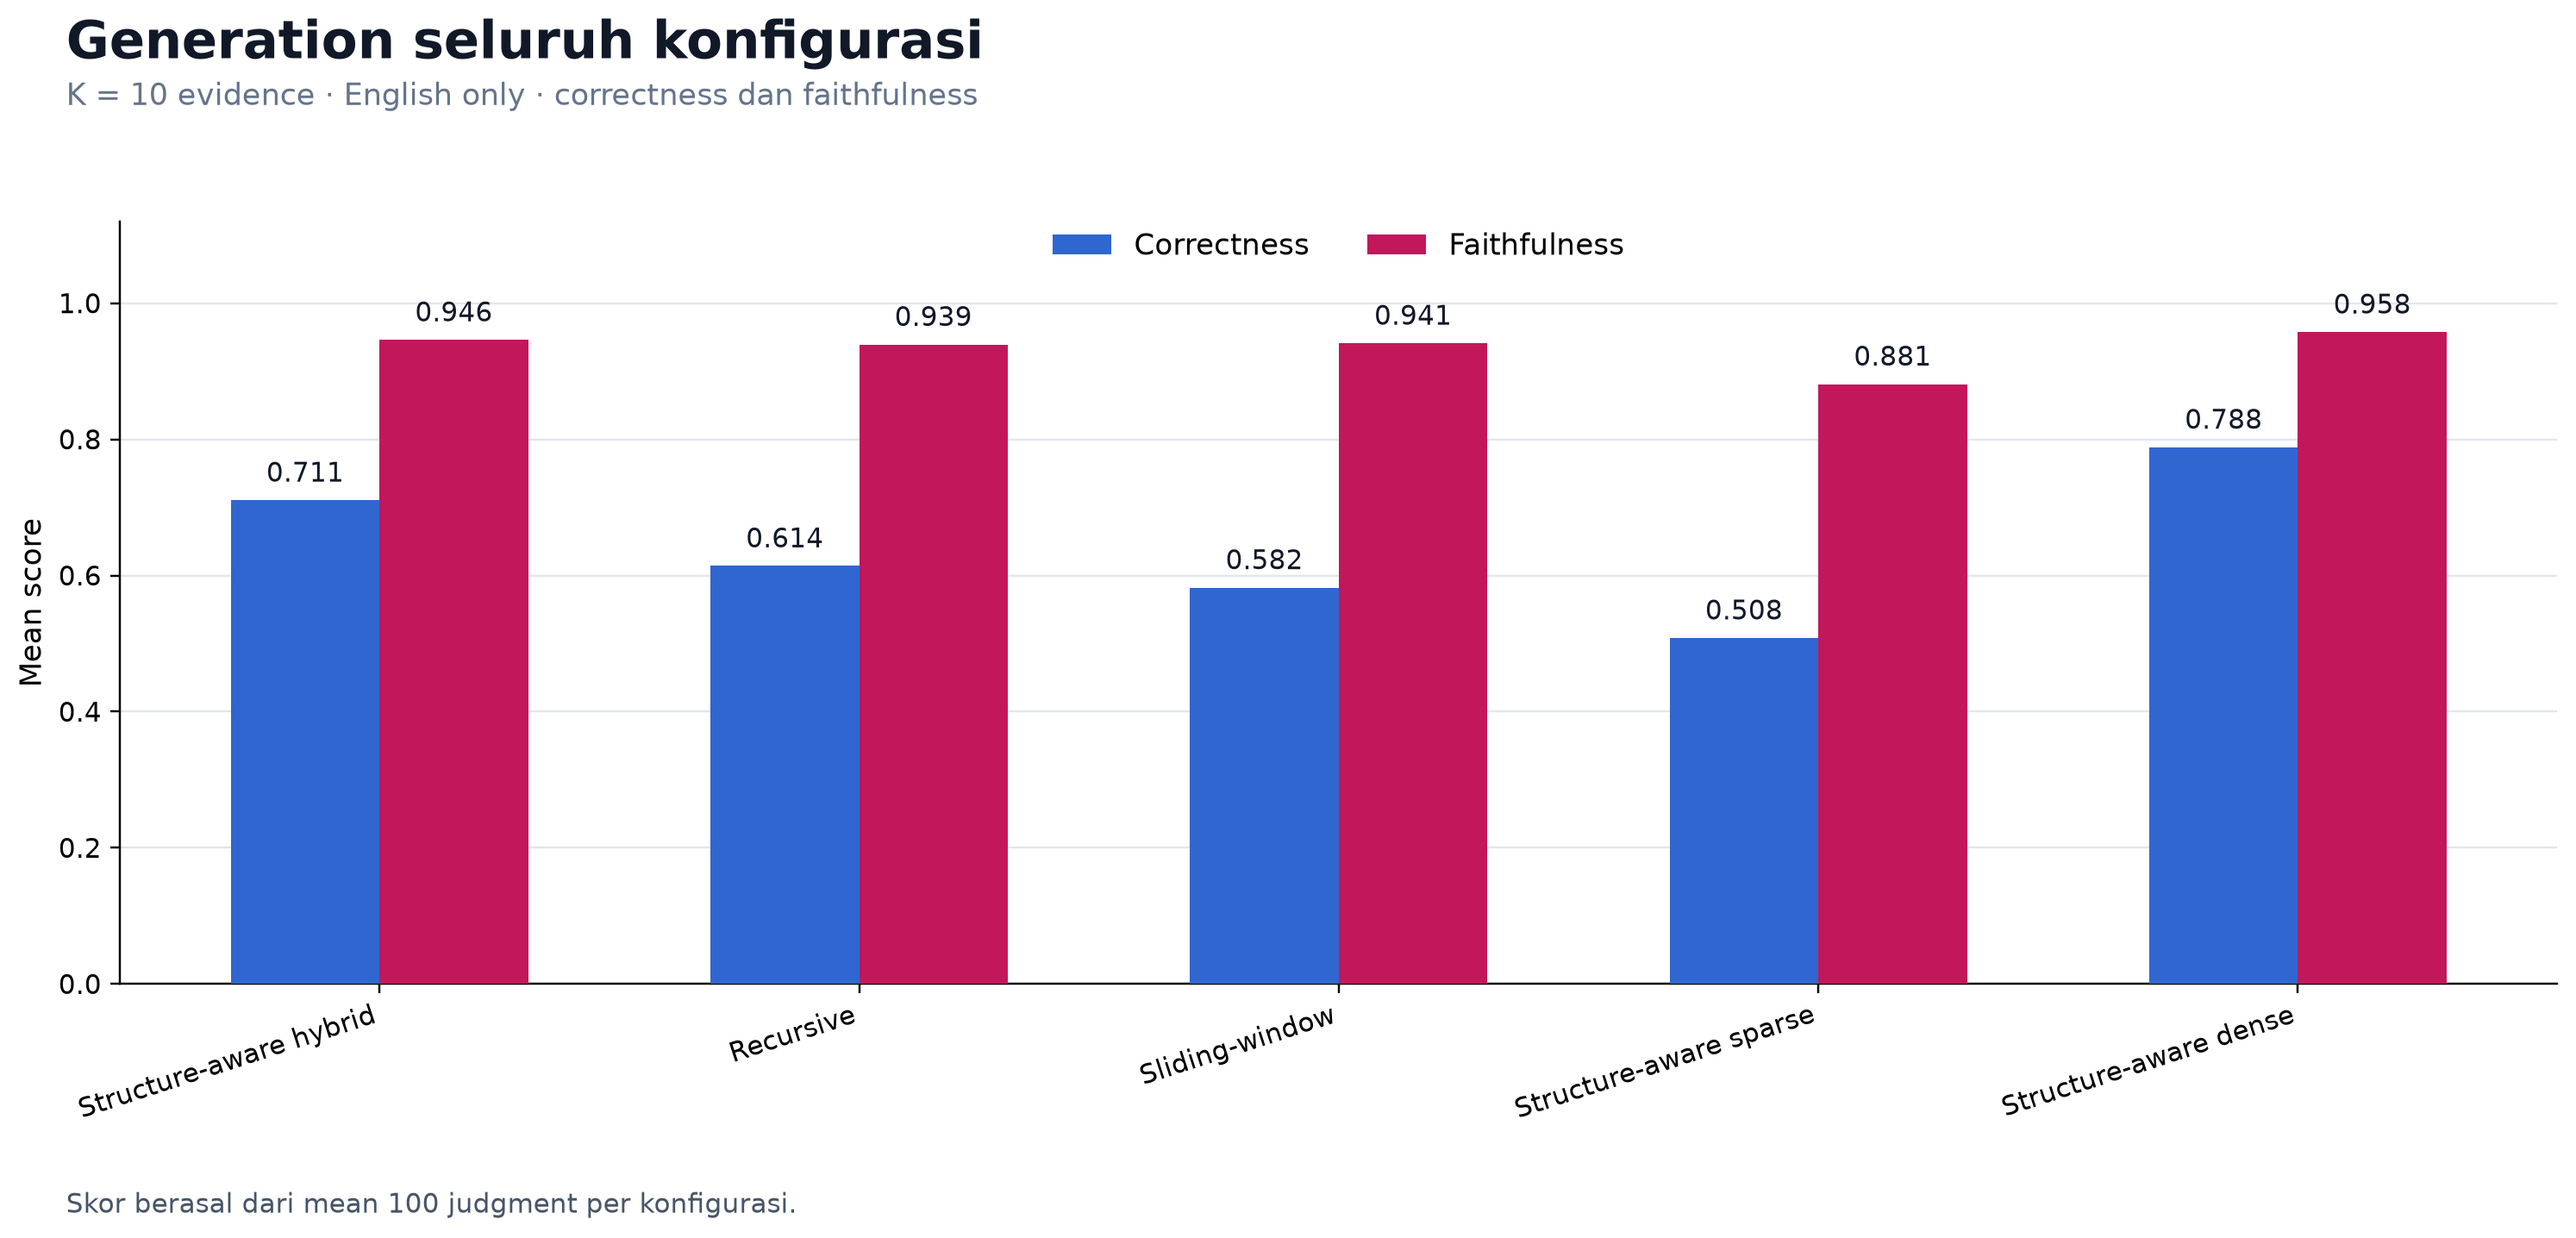
\includegraphics[width=\textwidth,height=0.43\textheight,keepaspectratio]{images/experiments/customer_service_revision/final_eda/generation-all.png}
\caption{\emph{Correctness} dan \emph{faithfulness} \emph{generation} untuk seluruh konfigurasi \emph{User Manual} dengan \(K = 10\)}
\label{fig:customer-generation-all-bar}
\end{figure}

Gambar~\ref{fig:customer-generation-all-bar} merupakan rekap dari pembahasan \emph{generation} per
komponen. \emph{Structure-aware} \emph{dense} memperoleh \emph{correctness} 0,788 dan \emph{faithfulness} 0,958, \emph{hybrid}
0,711 dan 0,946, \emph{recursive} 0,614 dan 0,939, \emph{sliding-window} 0,582 dan 0,941, sedangkan \emph{sparse}
0,508 dan 0,881. Urutan ini mengikuti kelengkapan dan penempatan \emph{evidence} yang telah terlihat
pada eksperimen \emph{retrieval}, bukan hasil penggabungan \emph{evidence} lintas konfigurasi.

\emph{Volume} \emph{token} \emph{generation} telah dirinci pada subbagian \emph{generation} \emph{chunker} dan \emph{indexer}. Gambar
berikut hanya memberikan pandangan gabungan. Estimasi menggunakan panjang \emph{evidence} dibagi empat
pada \(K = 10\), sehingga berbeda dari \emph{payload} kandidat \(K = 30\) yang digunakan untuk \emph{reranker}.

\begin{figure}[H]
\centering
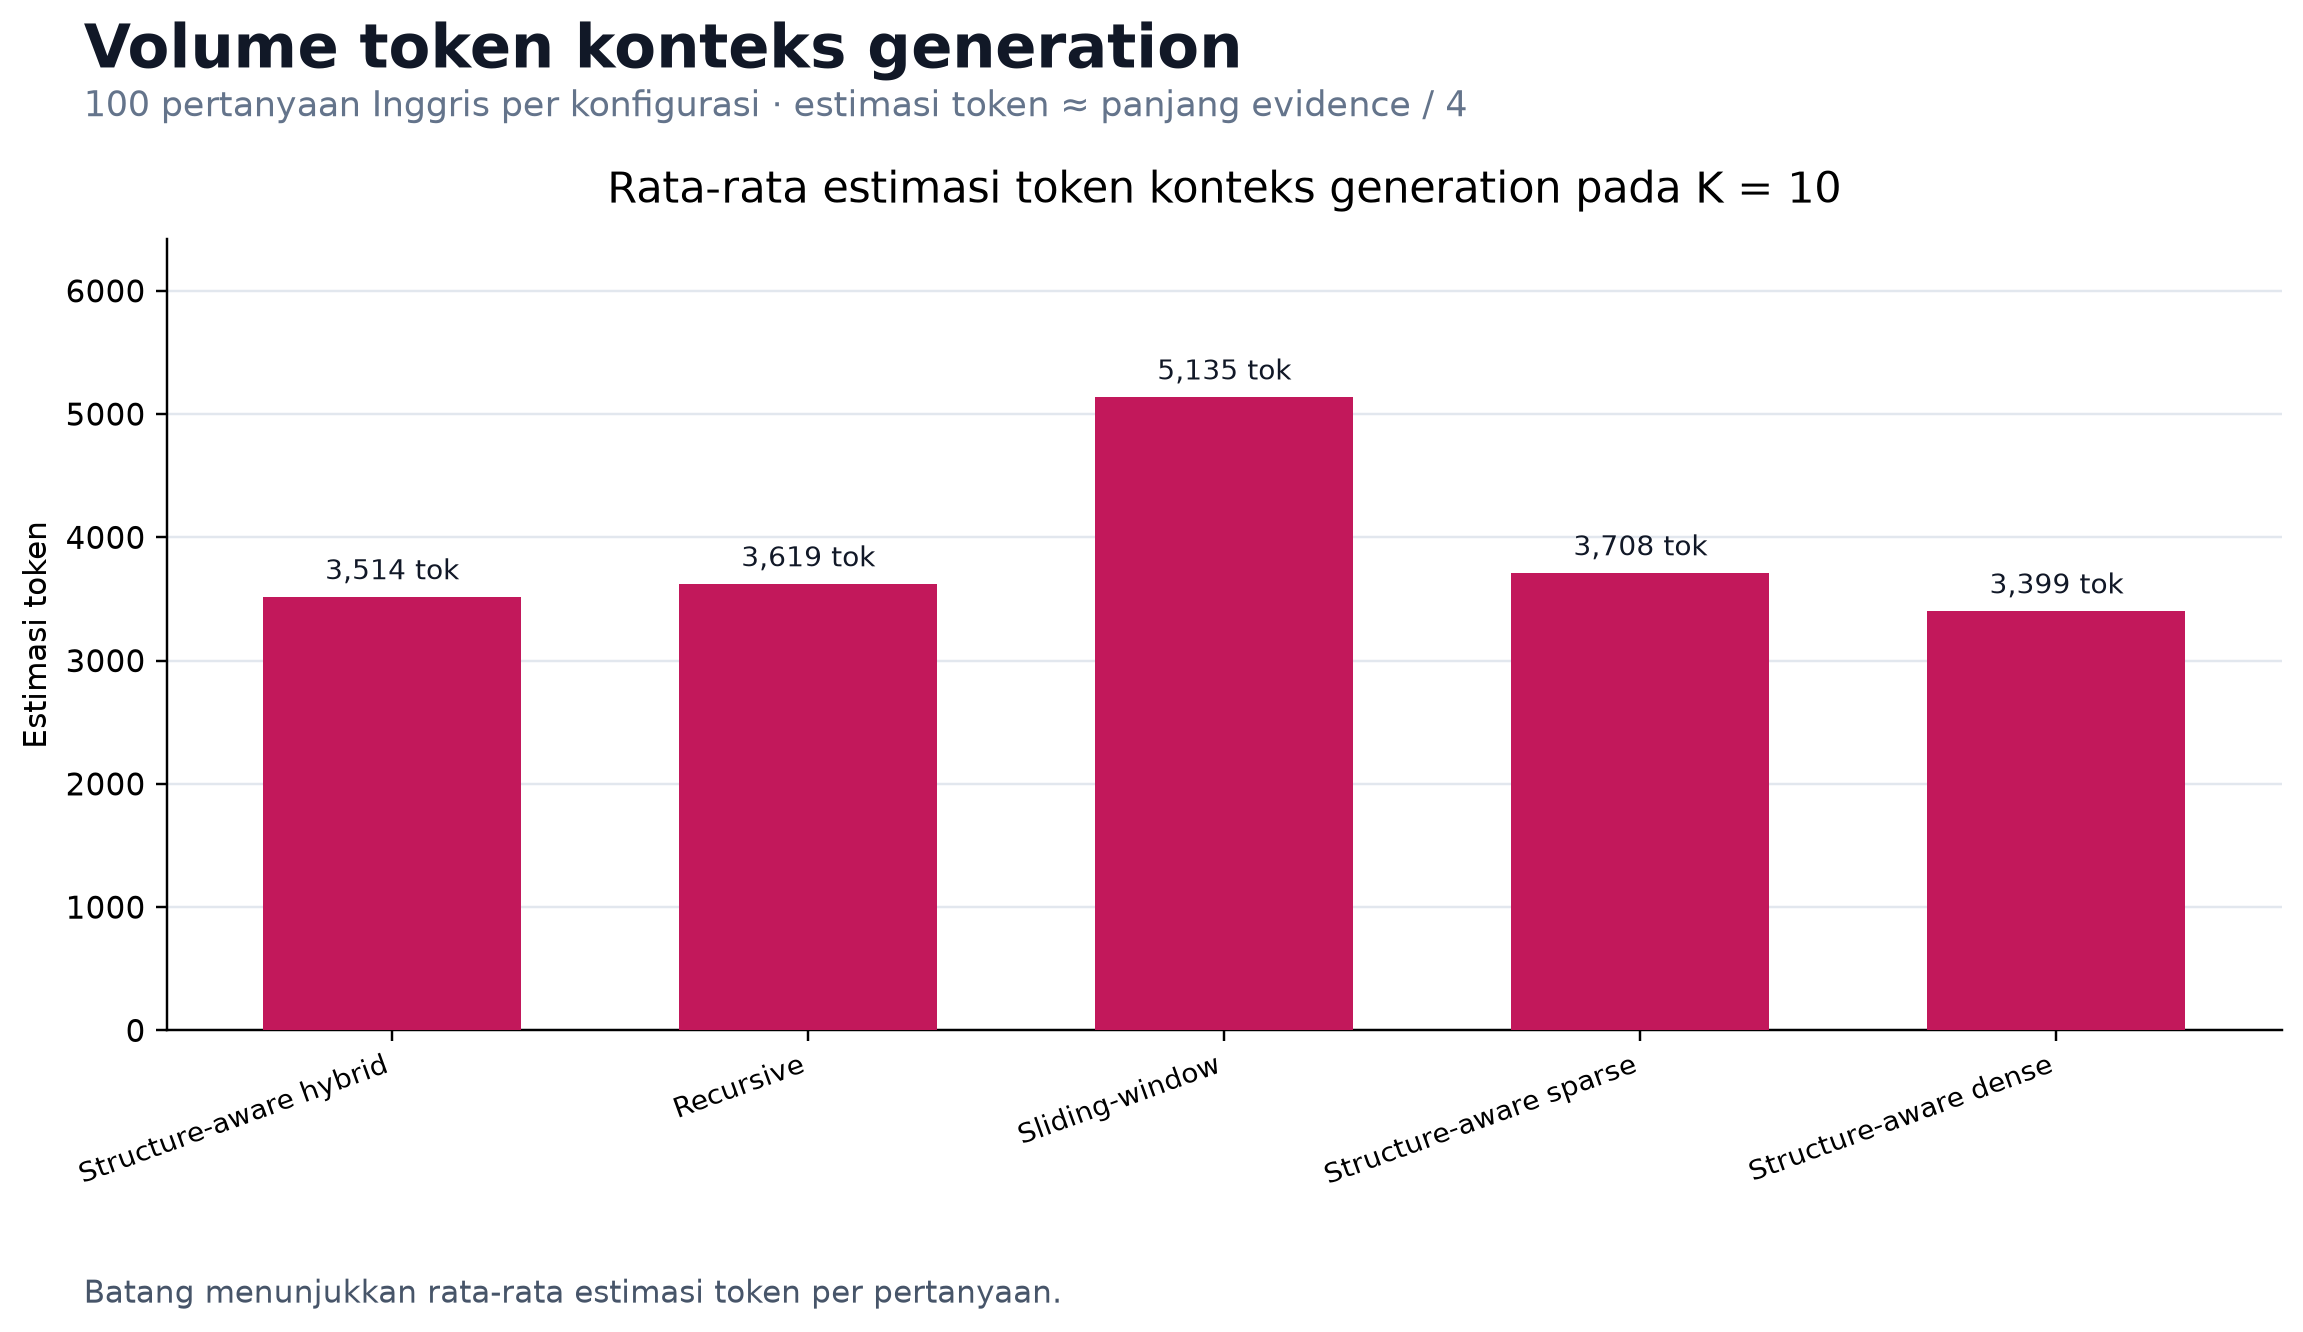
\includegraphics[width=\textwidth,height=0.55\textheight,keepaspectratio]{images/experiments/customer_service_revision/final_eda/generation-context-volume.png}
\caption{Rata-rata estimasi \emph{token} konteks \emph{generation} pada \(K = 10\)}
\label{fig:customer-generation-context-volume}
\end{figure}

\subsection{Analisis dan Keterbatasan Eksperimen}
\label{subsec:user-manual-analysis-limitations}

Hasil Inggris cenderung lebih tinggi karena bahasa manual sama dengan query, sedangkan query
Indonesia menguji lintas bahasa. Perbedaan paling besar terlihat pada \emph{sparse}, sementara \emph{dense}
menjaga jarak lintas bahasa yang lebih kecil. \emph{Retrieval} memakai \(K = 30\) dan \emph{generation}
\(K = 10\). Lima konfigurasi dibandingkan secara lokal, tanpa penggabungan hasil antarkonfigurasi
dan tanpa skor komposit. \emph{Dataset} terbatas pada sembilan manual, sehingga hasil ini menjelaskan
perilaku konfigurasi pada \emph{corpus} tersebut dan belum dapat dianggap sebagai ukuran semua manual
produk. \emph{Volume} \emph{payload} \emph{generation} dan \emph{reranker} dibaca sesuai tahapnya masing-masing, karena
keduanya menggunakan \emph{cutoff} dan tujuan yang berbeda.



% Updated \emph{legal} \emph{revision} section aligned with the \emph{User Manual} reporting structure.
\section{Eksperimen pada \emph{Use Case} Hukum}
\label{sec:eksperimen-legal-revision-updated}
\label{sec:eksperimen-legal-revision}

Eksperimen hukum menggunakan susunan pelaporan yang sama dengan eksperimen
\emph{User Manual}. Perbedaan khususnya adalah adanya eksperimen
\emph{knowledge-graph recall} untuk mengukur jangkauan dokumen yang terhubung.
Semua angka di bagian ini dihitung terpisah untuk setiap konfigurasi. Istilah
\emph{context reference} digunakan untuk menyebut konteks yang menjadi acuan
pertanyaan.

\subsection{Pembentukan \emph{Dataset} Eksperimen}
\label{subsec:legal-revision-dataset-updated}
\label{subsec:legal-revision-dataset}

\emph{Dataset} hukum berisi 25 pertanyaan yang disusun untuk eksperimen dan diverifikasi oleh ahli.
Referensi konteks setiap pertanyaan digunakan untuk memilih dokumen inti, kemudian ditambahkan
207 dokumen \emph{noise}.
\emph{Noise} dipilih melalui \emph{stratified} \emph{sampling} berdasarkan \emph{form group}, \emph{status}
peraturan, \emph{year band}, dan \emph{length band}. Dengan demikian, \emph{datasource} yang
digunakan oleh semua konfigurasi tetap berisi 256 dokumen dan tetap mewakili komposisi
frame \emph{vector} operasional.

\begin{table}[H]\centering\scriptsize
\caption{Cakupan \emph{datasource} eksperimen hukum}
\label{tab:legal-revision-dataset-updated}
\begin{tabularx}{\textwidth}{@{}>{\RaggedRight\arraybackslash}Xr@{}}
\toprule\textbf{Komponen} & \textbf{Jumlah}\\\midrule
Baris \emph{vector} siap pakai sebelum validasi & 4.459\\
Baris \emph{vector} valid & 4.453\\
Frame \emph{vector} operasional setelah penambahan referensi wajib & 4.462\\
Dokumen \emph{datasource} & 256\\
Dokumen yang memuat \emph{context reference} & 49\\
Dokumen \emph{noise} terstratifikasi & 207\\
Pertanyaan terverifikasi & 25\\
Baris referensi benchmark & 148\\
Jumlah unik \emph{context reference} & 144\\
Dokumen \emph{seed} unik & 45\\
\bottomrule\end{tabularx}
\end{table}

Frame operasional terdiri atas 4.462 dokumen setelah pemeriksaan dan penambahan
referensi wajib. Angka 148 dan 144 pada tabel menunjukkan jumlah baris referensi dan
konteks unik yang dipakai pada benchmark aktif.

Distribusi pertanyaan dilaporkan berdasarkan kategori isi pada 25
pertanyaan. Kategori tersebut bukan \emph{label} klasifikasi untuk \emph{retrieval}, tetapi
cara ringkas untuk memeriksa bahwa benchmark mencakup beberapa jenis kebutuhan
informasi hukum.

\begin{table}[H]\centering\scriptsize
\caption{Distribusi kategori pertanyaan hukum}
\label{tab:legal-question-category-distribution}
\begin{tabularx}{0.88\textwidth}{@{}>{\RaggedRight\arraybackslash}Xrr@{}}
\toprule\textbf{\emph{Question} \emph{category}} & \textbf{\emph{Questions}} & \textbf{Share}\\\midrule
Institutional establishment and \emph{status} & 6 & 24\%\\
Governance and authority & 4 & 16\%\\
Admissions and student access & 4 & 16\%\\
Academic staff and qualifications & 3 & 12\%\\
Quality assurance and reporting & 4 & 16\%\\
Compliance, conduct, and cooperation & 4 & 16\%\\
\bottomrule\end{tabularx}
\end{table}

\begin{figure}[H]\centering

\includegraphics[width=0.88\textwidth]{images/experiments/legal_revision/final_eda/question-category-distribution.png}
\caption{\emph{Legal} question distribution}
\label{fig:legal-question-category-distribution}
\end{figure}

Gambar~\ref{fig:legal-question-category-distribution} memperlihatkan bahwa
pertanyaan paling banyak berada pada kategori \emph{Institutional establishment and
status}, sedangkan lima kategori lain tetap terwakili. Komposisi ini berasal dari
pertanyaan terverifikasi, sehingga \emph{noise} hanya memperluas \emph{datasource} dan tidak mengubah
pertanyaan maupun referensi yang harus ditemukan.

\begin{figure}[H]\centering
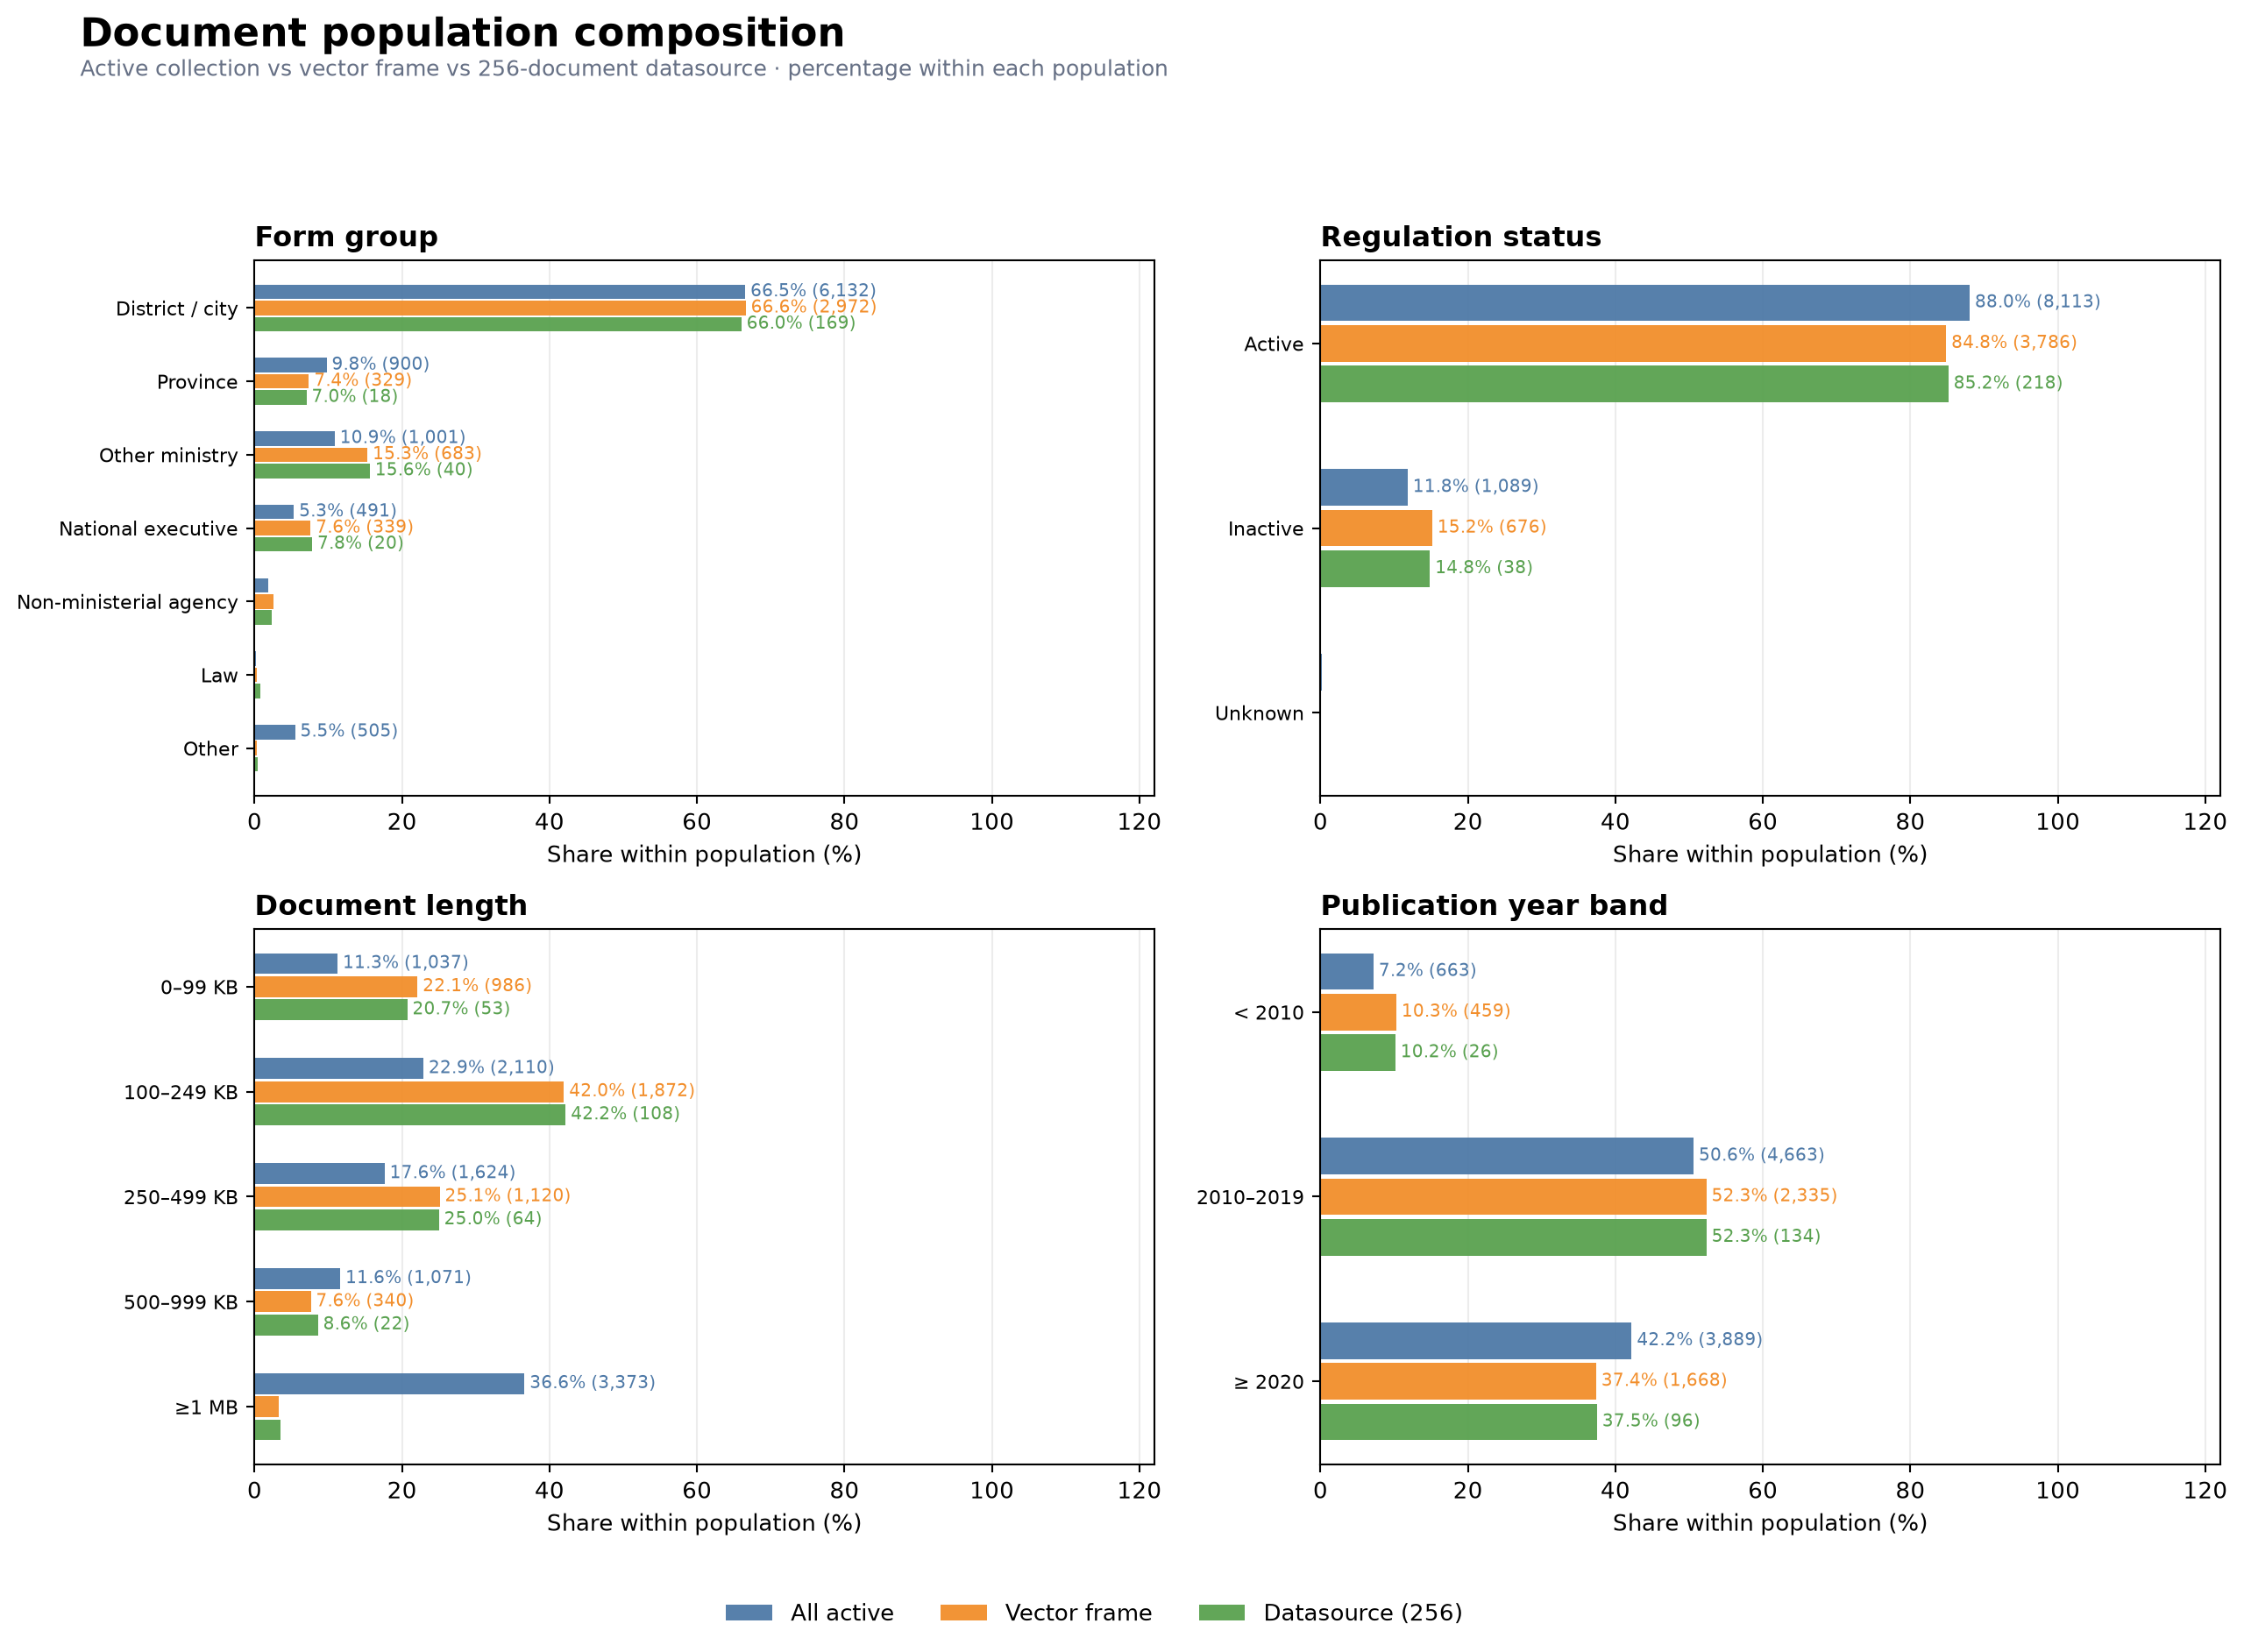
\includegraphics[width=0.92\textwidth]{images/experiments/legal_revision/final_eda/corpus-composition-comparison.png}
\caption{Document population composition across the four stratification dimensions}
\label{fig:legal-corpus-composition-comparison}
\end{figure}

Gambar~\ref{fig:legal-corpus-composition-comparison} membandingkan proporsi di
dalam tiga populasi, yaitu seluruh dokumen aktif (9.215), \emph{vector} \emph{frame} operasional
(4.462), dan \emph{datasource} akhir (256 dokumen yang terdiri atas 49 dokumen yang
memuat \emph{context reference} dan 207 dokumen \emph{noise}). Keempat panel menggunakan
\emph{form group}, \emph{status} peraturan, length bin berbasis ukuran \emph{byte}, dan \emph{year band}. Pola
\emph{datasource} akhir mengikuti \emph{vector} \emph{frame} pada keempat dimensi. Perbedaan terhadap
seluruh dokumen aktif menunjukkan bahwa \emph{sampling} dilakukan dari ruang \emph{vector}
yang dipakai \emph{parser}, bukan dari seluruh dokumen aktif.

\subsection{Konfigurasi dan Metodologi Eksperimen}
\label{subsec:legal-revision-config-updated}
\label{subsec:legal-revision-config}

Metrik \emph{retrieval} dan \emph{generation} mengikuti definisi pada eksperimen \emph{User Manual}.
\emph{Recall} merupakan metrik utama karena mengukur cakupan \emph{context reference} yang
ditemukan. \emph{Precision}, \emph{MRR}, dan \emph{NDCG} menjadi metrik pendukung untuk membaca kepadatan
kandidat dan kualitas urutannya sebelum kandidat diproses oleh komponen \emph{downstream}.
\emph{Correctness} mengukur kelengkapan jawaban, sedangkan \emph{faithfulness} mengukur apakah klaim
jawaban didukung \emph{evidence} yang dikirim. \emph{NDCG} dinilai dengan \emph{framework} \emph{RAG} menggunakan
\emph{model} \texttt{openai/gpt-5.6-luna} dengan \emph{reasoning effort} \texttt{high} dan \emph{label} relevansi 0, 1, dan 2.

\begin{table}[H]\centering\scriptsize
\caption{Konfigurasi eksperimen hukum}
\label{tab:legal-revision-config-updated}
\begin{tabularx}{\textwidth}{@{}>{\RaggedRight\arraybackslash}p{3.6cm}>{\RaggedRight\arraybackslash}p{4.5cm}>{\RaggedRight\arraybackslash}X@{}}
\toprule\textbf{Konfigurasi} & \textbf{\emph{Chunker}} & \textbf{\emph{Indexer}}\\\midrule
\emph{Legal-structure} \emph{dense} & \emph{Legal} structure, 512 karakter, ayat \emph{overlap} 0, \emph{parent hydration} & \emph{Dense} BAAI/\emph{BGE-M3}\\
\emph{Recursive} & \emph{Recursive}, 512 karakter, \emph{overlap} 51 & \emph{Dense} BAAI/\emph{BGE-M3}\\
\emph{Baseline chunker: Sliding} & \emph{Sliding window}, 512 karakter, \emph{overlap} 51 & \emph{Dense} BAAI/\emph{BGE-M3}\\
\emph{Baseline indexer: Structure-aware sparse} & \emph{Legal} structure, 512 karakter, ayat \emph{overlap} 0, \emph{parent hydration} & \emph{Sparse}\\
\emph{Structure-aware} \emph{hybrid} & \emph{Legal} structure, 512 karakter, ayat \emph{overlap} 0, \emph{parent hydration} & \emph{Dense}+\emph{sparse} RRF\\
\bottomrule\end{tabularx}
\end{table}

\emph{Parser} menggunakan \emph{native} \emph{text} tanpa \emph{OCR}. \emph{Reranker}, \emph{guardrail}, \emph{context-PII}, dan
\emph{knowledge graph} dimatikan pada \emph{direct} \emph{retrieval} agar lima konfigurasi dibandingkan
pada jalur yang sama. \emph{Sweep} \emph{retrieval} memakai \(K = 5\) sampai \(K = 60\). \emph{Generation}
menggunakan sepuluh \emph{evidence} teratas, yaitu \(K = 10\), sedangkan \(K = 30\) digunakan
sebagai \emph{cutoff} kandidat bersama sebelum tahap \emph{downstream}.

\subsection{Eksperimen Strategi \emph{Chunker}}
\label{subsec:legal-revision-chunker-updated}
\label{subsec:legal-revision-chunker}

Eksperimen ini mempertahankan \emph{datasource}, \emph{parser}, pemetaan \emph{context reference}, \emph{model}
\emph{embedding}, dan \emph{dense} \emph{indexer}. Hanya strategi \emph{chunker} yang diubah. \emph{Sliding} digunakan
sebagai \emph{baseline} karena merupakan pendekatan \emph{fixed-window} yang paling sederhana.
Perbandingan ini menunjukkan apakah struktur hukum yang dipertahankan oleh
\emph{Legal-structure} \emph{dense} dapat mengalahkan \emph{baseline} tersebut.

\begin{table}[H]\centering\scriptsize
\caption{\emph{Retrieval} kelompok \emph{chunker} \emph{legal} pada \(K = 30\)}
\label{tab:legal-revision-chunker-updated}
\begin{tabularx}{\textwidth}{@{}>{\RaggedRight\arraybackslash}p{4.4cm}rrrr@{}}
\toprule\textbf{Konfigurasi} & \textbf{\emph{Recall}} & \textbf{\emph{Precision}} & \textbf{\emph{NDCG}} & \textbf{\emph{MRR}}\\\midrule
\emph{Legal-structure} \emph{dense} & \textbf{0,6854} & \textbf{0,1520} & 0,5040 & \textbf{0,5240}\\
\emph{Recursive} & 0,6730 & 0,1453 & 0,4909 & 0,4937\\
\emph{Baseline chunker: Sliding} & 0,6345 & 0,1507 & \textbf{0,5042} & 0,4626\\
\bottomrule\end{tabularx}
\end{table}

\begin{figure}[H]\centering

\includegraphics[width=\textwidth,height=0.44\textheight,keepaspectratio]{images/experiments/legal_revision/final_eda/recall-chunker.png}
\caption{\emph{Recall} menurut jumlah kandidat untuk konfigurasi \emph{chunker} \emph{legal}}
\label{fig:legal-revision-recall-chunker-updated}
\end{figure}

Pada Gambar~\ref{fig:legal-revision-recall-chunker-updated}, \emph{Legal-structure} \emph{dense}
mencapai \emph{recall} 0,6854 pada \(K = 30\), \emph{Recursive} 0,6730, dan \emph{Sliding} 0,6345.
Dengan demikian, \emph{structure-aware} \emph{chunker} mengalahkan \emph{baseline} \emph{Sliding} sebesar
0,0509 dan hanya berbeda 0,0124 dari \emph{Recursive}. Selisih yang tidak terlalu jauh ini masuk akal
karena ketiga konfigurasi memakai \emph{datasource}, parser, model \emph{embedding}, \emph{dense indexer}, dan
144 \emph{context reference} benchmark aktif yang sama. Perubahan eksperimen hanya berada pada cara batas teks dibentuk.
\emph{Legal-structure} lebih unggul karena isi ayat tetap disertai identitas bagian hukum yang menjelaskan
subjek, kewenangan, atau persyaratannya. \emph{Recursive} masih dekat karena kalimat yang bersebelahan sering
berada dalam kandidat yang sama, tetapi bagian dari satu persyaratan dapat terpisah. \emph{Sliding} tetap
kompetitif karena \emph{overlap} dapat menangkap referensi di sekitar batas jendela, walaupun beberapa kandidat
yang berdekatan membawa teks yang berulang. Hasil ini menunjukkan keunggulan konsisten pada \emph{coverage},
bukan klaim perbedaan yang telah diuji secara statistik.

\begin{figure}[H]\centering

\includegraphics[width=\textwidth,height=0.44\textheight,keepaspectratio]{images/experiments/legal_revision/final_eda/precision-chunker.png}
\caption{\emph{Precision} menurut jumlah kandidat untuk konfigurasi \emph{chunker} \emph{legal}}
\label{fig:legal-revision-precision-chunker-updated}
\end{figure}

Gambar~\ref{fig:legal-revision-precision-chunker-updated} menunjukkan \emph{precision}
yang cenderung turun ketika \(K\) diperbesar. Penyebabnya adalah jumlah kandidat
bertambah lebih cepat daripada \emph{context reference} baru yang ditemukan. Pada \(K = 30\),
\emph{Legal-structure} \emph{dense} memiliki nilai 0,1520, \emph{Sliding} 0,1507, dan \emph{Recursive} 0,1453.
Nilai \emph{dense} dan \emph{Sliding} hampir sama sehingga kepadatan kandidat tidak menjelaskan seluruh
keunggulan \emph{recall}. Perbedaannya justru terlihat pada berapa banyak referensi berbeda yang dapat
dikumpulkan dari kandidat tersebut.

\begin{figure}[H]\centering

\includegraphics[width=\textwidth,height=0.44\textheight,keepaspectratio]{images/experiments/legal_revision/final_eda/ndcg-chunker.png}
\caption{\emph{NDCG} menurut jumlah kandidat untuk konfigurasi \emph{chunker} \emph{legal}}
\label{fig:legal-revision-ndcg-chunker-updated}
\end{figure}

Gambar~\ref{fig:legal-revision-ndcg-chunker-updated} memperlihatkan bahwa \emph{NDCG}
\emph{Sliding} pada \(K = 30\) adalah 0,5042, hanya 0,0002 di atas \emph{Legal-structure} \emph{dense}
yang bernilai 0,5040. \emph{Recursive} bernilai 0,4909. Kedekatan \emph{Sliding} dan \emph{dense} berarti
keduanya dapat menempatkan setidaknya satu kandidat yang relevan di posisi awal. Namun, \emph{NDCG} memberi
penekanan pada posisi awal, sedangkan \emph{recall} menghitung seluruh referensi yang ditemukan. Karena itu,
\emph{Sliding} dapat hampir menyamai \emph{NDCG} tanpa menyamai kelengkapan \emph{recall}.

\begin{figure}[H]\centering

\includegraphics[width=\textwidth,height=0.44\textheight,keepaspectratio]{images/experiments/legal_revision/final_eda/mrr-chunker.png}
\caption{\emph{MRR} menurut jumlah kandidat untuk konfigurasi \emph{chunker} \emph{legal}}
\label{fig:legal-revision-mrr-chunker-updated}
\end{figure}

Pada Gambar~\ref{fig:legal-revision-mrr-chunker-updated}, \emph{MRR} \emph{Legal-structure} \emph{dense}
adalah 0,5240, \emph{Recursive} 0,4937, dan \emph{Sliding} 0,4626. Selisih \emph{dense} terhadap
\emph{Recursive} adalah 0,0303 dan terhadap \emph{Sliding} adalah 0,0614. Ini menunjukkan bahwa kandidat
pertama yang berguna lebih sering muncul di posisi awal pada representasi yang mempertahankan struktur hukum.
\emph{MRR} tetap hanya membaca posisi \emph{reference} pertama, sehingga tidak menunjukkan kelengkapan seluruh
\emph{reference}.

\begin{figure}[H]\centering
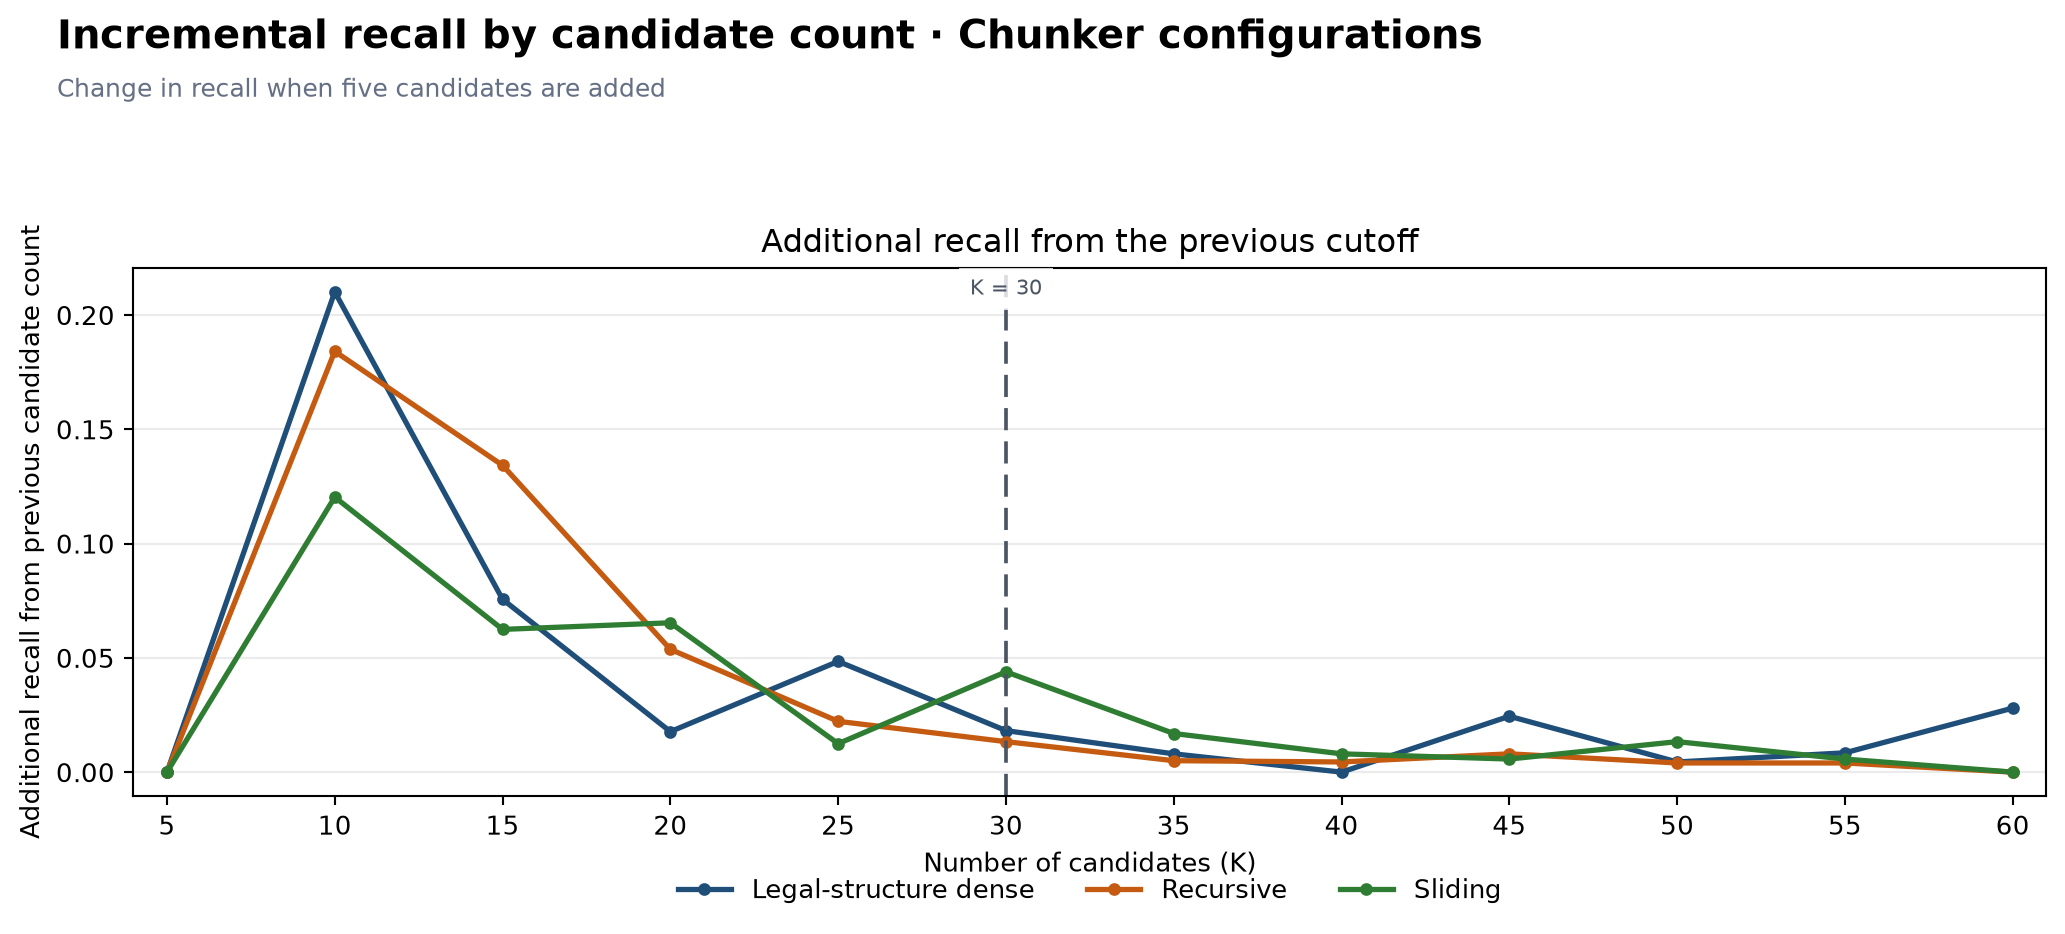
\includegraphics[width=\textwidth,height=0.44\textheight,keepaspectratio]{images/experiments/legal_revision/final_eda/recall-marginal-delta-chunker.png}
\caption{Tambahan \emph{recall} menurut jumlah kandidat untuk konfigurasi \emph{chunker} \emph{legal}}
\label{fig:legal-revision-recall-delta-chunker-updated}
\end{figure}

Gambar~\ref{fig:legal-revision-recall-delta-chunker-updated} menunjukkan tambahan
\emph{recall} setiap kali \emph{cutoff} dinaikkan. Perubahannya besar pada bagian awal kurva dan menjadi
lebih tidak teratur setelah \(K = 30\). Dengan kata lain, \(K = 30\) merupakan titik kerja lokal yang sudah
memberi sebagian besar \emph{coverage} yang mudah ditemukan, sedangkan kandidat setelahnya membentuk ekor
tambahan yang tidak selalu memberi referensi baru. \(K = 30\) dipakai untuk menyediakan pilihan yang cukup
untuk \emph{reranker} \emph{downstream} tanpa mengirim seluruh ekor kandidat.

\begin{figure}[H]\centering

\includegraphics[width=\textwidth,height=0.44\textheight,keepaspectratio]{images/experiments/legal_revision/final_eda/metrics-at-sweet-spot-chunker.png}
\caption{Metrik \emph{retrieval} untuk konfigurasi \emph{chunker} \emph{legal} pada \(K = 30\)}
\label{fig:legal-revision-sweet-chunker-updated}
\end{figure}

Gambar~\ref{fig:legal-revision-sweet-chunker-updated} merangkum empat metrik pada
\emph{cutoff} yang sama. \emph{Legal-structure} \emph{dense} unggul pada \emph{recall} 0,6854, \emph{precision}
0,1520, dan \emph{MRR} 0,5240. \emph{Sliding} hanya unggul tipis pada \emph{NDCG} dengan 0,5042 berbanding
0,5040. Karena tujuan komponen \emph{chunker} adalah menjaga \emph{coverage} \emph{context reference}, hasil ini
mendukung pemilihan \emph{Legal-structure} \emph{dense} sebagai konfigurasi utama. Keunggulannya tidak berasal
dari jumlah kandidat yang lebih banyak, tetapi dari kandidat yang lebih sering membawa konteks hukum yang lengkap.

\emph{Generation} kelompok \emph{chunker} menggunakan \(K = 10\) \emph{evidence}. \emph{Correctness}
\emph{Legal-structure} \emph{dense}, \emph{Recursive}, dan \emph{Sliding} berturut-turut adalah 0,690, 0,556,
dan 0,575. \emph{Faithfulness} berturut-turut adalah 0,972, 0,979, dan 0,979.

\begin{figure}[H]\centering

\includegraphics[width=\textwidth,height=0.44\textheight,keepaspectratio]{images/experiments/legal_revision/final_eda/generation-chunker.png}
\caption{\emph{Correctness} dan \emph{faithfulness} konfigurasi \emph{chunker} \emph{legal} pada \(K = 10\)}
\label{fig:legal-revision-generation-chunker-updated}
\end{figure}

Gambar~\ref{fig:legal-revision-generation-chunker-updated} menunjukkan bahwa
\emph{Legal-structure} \emph{dense} menghasilkan \emph{correctness} tertinggi, yaitu 0,690, sedangkan
\emph{Recursive} dan \emph{Sliding} masing-masing 0,556 dan 0,575. \emph{Faithfulness} tetap tinggi pada
ketiga konfigurasi, yaitu 0,972, 0,979, dan 0,979. Jadi perbedaannya terutama berada pada kelengkapan
\emph{evidence}, bukan pada dukungan terhadap klaim yang sudah ditulis. Rata-rata \emph{payload} \(K = 10\)
yang dikirim adalah sekitar 2.316 token untuk \emph{dense}, 1.335 token untuk \emph{Recursive}, dan 1.475 token
untuk \emph{Sliding}. Estimasi token dihitung dari panjang \emph{evidence} yang benar-benar dikirim dibagi empat.
\emph{Sliding} membawa lebih banyak token daripada \emph{Recursive}, tetapi sebagian volumenya berasal dari teks
berdekatan yang berulang. Karena itu, volume token yang lebih besar tidak otomatis menghasilkan jawaban yang lebih
lengkap.

\subsection{Eksperimen Strategi \emph{Indexer}}
\label{subsec:legal-revision-indexer-updated}
\label{subsec:legal-revision-indexer}

Eksperimen \emph{indexer} mempertahankan \emph{Legal-structure} \emph{chunker}, \emph{datasource}, \emph{parser}, dan
pemetaan \emph{context reference}. Hanya \emph{indexer} yang diubah. \emph{Structure-aware} \emph{sparse} menjadi
\emph{baseline} \emph{indexer} karena pencarian leksikal merupakan pendekatan paling sederhana.
\emph{Dense} dan \emph{hybrid} kemudian dibandingkan dengan \emph{baseline} tersebut.

\begin{table}[H]\centering\scriptsize
\caption{\emph{Retrieval} kelompok \emph{indexer} \emph{legal} pada \(K = 30\)}
\label{tab:legal-revision-indexer-updated}
\begin{tabularx}{\textwidth}{@{}>{\RaggedRight\arraybackslash}p{4.4cm}rrrr@{}}
\toprule\textbf{Konfigurasi} & \textbf{\emph{Recall}} & \textbf{\emph{Precision}} & \textbf{\emph{NDCG}} & \textbf{\emph{MRR}}\\\midrule
\emph{Legal-structure} \emph{dense} & \textbf{0,6854} & \textbf{0,1520} & \textbf{0,5040} & 0,5240\\
\emph{Baseline indexer: Structure-aware sparse} & 0,6381 & 0,1253 & 0,4262 & 0,4613\\
\emph{Structure-aware} \emph{hybrid} & 0,6412 & 0,1307 & 0,4797 & \textbf{0,5439}\\
\bottomrule\end{tabularx}
\end{table}

\begin{figure}[H]\centering

\includegraphics[width=\textwidth,height=0.44\textheight,keepaspectratio]{images/experiments/legal_revision/final_eda/recall-indexer.png}
\caption{\emph{Recall} menurut jumlah kandidat untuk konfigurasi \emph{indexer} \emph{legal}}
\label{fig:legal-revision-recall-indexer-updated}
\end{figure}

Gambar~\ref{fig:legal-revision-recall-indexer-updated} menunjukkan \emph{dense} sebagai
konfigurasi dengan \emph{coverage} tertinggi pada \(K = 30\), yaitu 0,6854. \emph{Hybrid} mencapai
0,6412 dan \emph{sparse} 0,6381. \emph{Dense} mengalahkan \emph{baseline} \emph{sparse} sebesar 0,0473 \emph{recall},
sedangkan \emph{hybrid} hanya 0,0031 di atas \emph{sparse}. Selisih \emph{dense} terhadap \emph{hybrid} juga
tidak besar secara absolut, yaitu 0,0442, karena keduanya tetap memakai teks \emph{chunk} dan \emph{datasource}
yang sama. Perbedaan utamanya adalah cara mencocokkan pertanyaan dengan redaksi dokumen. \emph{Dense} dapat
menjembatani istilah yang berbeda tetapi bermakna sama. \emph{Sparse} lebih bergantung pada kata yang sama,
sedangkan \emph{hybrid} menambahkan sinyal leksikal ke sinyal semantik sehingga membantu beberapa pertanyaan,
namun tidak selalu mempertahankan semua referensi berbeda dalam tiga puluh kandidat pertama.

\begin{figure}[H]\centering

\includegraphics[width=\textwidth,height=0.44\textheight,keepaspectratio]{images/experiments/legal_revision/final_eda/precision-indexer.png}
\caption{\emph{Precision} menurut jumlah kandidat untuk konfigurasi \emph{indexer} \emph{legal}}
\label{fig:legal-revision-precision-indexer-updated}
\end{figure}

\emph{Precision} pada Gambar~\ref{fig:legal-revision-precision-indexer-updated} menurun ketika
lebih banyak kandidat diteruskan. Pada \(K = 30\), \emph{dense} memperoleh 0,1520, \emph{hybrid} 0,1307,
dan \emph{sparse} 0,1253. Nilai \emph{dense} yang lebih tinggi berarti lebih banyak kandidat pada cutoff yang
sama membawa referensi yang dibutuhkan. \emph{Sparse} memiliki kepadatan terendah karena kecocokan kata literal
lebih mudah memasukkan dokumen yang memiliki istilah serupa tetapi tidak memuat konteks yang ditandai.
\emph{Hybrid} memperbaiki kepadatan terhadap \emph{sparse}, tetapi masih berada di bawah \emph{dense}.

\begin{figure}[H]\centering

\includegraphics[width=\textwidth,height=0.44\textheight,keepaspectratio]{images/experiments/legal_revision/final_eda/ndcg-indexer.png}
\caption{\emph{NDCG} menurut jumlah kandidat untuk konfigurasi \emph{indexer} \emph{legal}}
\label{fig:legal-revision-ndcg-indexer-updated}
\end{figure}

Pada Gambar~\ref{fig:legal-revision-ndcg-indexer-updated}, \emph{NDCG} \emph{dense} adalah 0,5040,
\emph{hybrid} 0,4797, dan \emph{sparse} 0,4262. Selisih \emph{dense} terhadap \emph{sparse} adalah 0,0778,
sedangkan \emph{hybrid} memperbaiki \emph{sparse} sebesar 0,0535. Artinya, penggabungan sinyal membantu
menempatkan kandidat yang lebih relevan di bagian atas. Namun, urutan yang lebih baik tidak otomatis membuat
semua referensi ditemukan. Karena itu \emph{hybrid} tetap berada di bawah \emph{dense} pada \emph{recall}.

\begin{figure}[H]\centering

\includegraphics[width=\textwidth,height=0.44\textheight,keepaspectratio]{images/experiments/legal_revision/final_eda/mrr-indexer.png}
\caption{\emph{MRR} menurut jumlah kandidat untuk konfigurasi \emph{indexer} \emph{legal}}
\label{fig:legal-revision-mrr-indexer-updated}
\end{figure}

\emph{MRR} pada Gambar~\ref{fig:legal-revision-mrr-indexer-updated} adalah 0,5240 untuk
\emph{dense}, 0,4613 untuk \emph{sparse}, dan 0,5439 untuk \emph{hybrid}. \emph{Hybrid} mempunyai hit pertama
terbaik, dengan kenaikan 0,0826 dibandingkan \emph{baseline} \emph{sparse} dan 0,0199 dibandingkan \emph{dense}.
Hal ini menunjukkan bahwa sinyal leksikal dan semantik bersama-sama dapat membawa satu konteks yang cocok ke
posisi awal. Hasil tersebut tidak berarti \emph{hybrid} menemukan paling banyak referensi. Untuk tujuan utama
\emph{coverage}, \emph{dense} tetap lebih baik.

\begin{figure}[H]\centering

\includegraphics[width=\textwidth,height=0.44\textheight,keepaspectratio]{images/experiments/legal_revision/final_eda/recall-marginal-delta-indexer.png}
\caption{Tambahan \emph{recall} menurut jumlah kandidat untuk konfigurasi \emph{indexer} \emph{legal}}
\label{fig:legal-revision-recall-delta-indexer-updated}
\end{figure}

Delta \emph{recall} pada Gambar~\ref{fig:legal-revision-recall-delta-indexer-updated} paling
besar pada \emph{cutoff} awal dan menjadi lebih tidak teratur setelah kandidat bertambah. Beberapa konfigurasi
masih memperoleh referensi baru pada cutoff yang lebih tinggi, tetapi tambahan tersebut muncul sebagai ekor dan
tidak konsisten untuk semua pertanyaan. Setelah mendekati \(K = 30\), \emph{cutoff} ini menjadi titik kerja yang
masih menyediakan opsi bagi \emph{reranker} tanpa membawa seluruh kandidat ekor.

\begin{figure}[H]\centering

\includegraphics[width=\textwidth,height=0.44\textheight,keepaspectratio]{images/experiments/legal_revision/final_eda/metrics-at-sweet-spot-indexer.png}
\caption{Metrik \emph{retrieval} untuk konfigurasi \emph{indexer} \emph{legal} pada \(K = 30\)}
\label{fig:legal-revision-sweet-indexer-updated}
\end{figure}

Gambar~\ref{fig:legal-revision-sweet-indexer-updated} memperlihatkan trade-off \emph{indexer}.
\emph{Dense} memberi \emph{recall} 0,6854, \emph{precision} 0,1520, dan \emph{NDCG} 0,5040. \emph{Hybrid} memberi
\emph{MRR} tertinggi, yaitu 0,5439, tetapi \emph{recall}-nya 0,6412. \emph{Baseline} \emph{sparse} berada di bawah
keduanya pada metrik-metrik tersebut. Dengan demikian, \emph{dense} mengalahkan baseline pada kelengkapan
referensi, sedangkan \emph{hybrid} mengalahkannya pada posisi hit pertama. Pemilihan konfigurasi tetap mengikuti
tujuan utama komponen, yaitu mengumpulkan \emph{context reference} sebanyak mungkin.

\emph{Generation} kelompok \emph{indexer} pada \(K = 10\) memperoleh \emph{correctness} 0,690 untuk \emph{dense},
0,578 untuk \emph{sparse}, dan 0,664 untuk \emph{hybrid}. \emph{Faithfulness} berturut-turut adalah 0,972,
0,982, dan 0,982.

\begin{figure}[H]\centering

\includegraphics[width=\textwidth,height=0.44\textheight,keepaspectratio]{images/experiments/legal_revision/final_eda/generation-indexer.png}
\caption{\emph{Correctness} dan \emph{faithfulness} konfigurasi \emph{indexer} \emph{legal} pada \(K = 10\)}
\label{fig:legal-revision-generation-indexer-updated}
\end{figure}

Gambar~\ref{fig:legal-revision-generation-indexer-updated} menunjukkan bahwa \emph{dense}
memberikan \emph{correctness} tertinggi, yaitu 0,690, sedangkan \emph{sparse} 0,578 dan \emph{hybrid} 0,664.
\emph{Faithfulness} \emph{sparse} dan \emph{hybrid} sedikit lebih tinggi, yaitu 0,982, dibandingkan 0,972 pada
\emph{dense}. Artinya, klaim yang ditulis oleh kedua konfigurasi tersebut tetap didukung oleh \emph{evidence},
tetapi \emph{evidence} tersebut belum selalu mencakup semua informasi jawaban. Rata-rata \emph{payload} \(K = 10\)
adalah sekitar 2.316 token untuk \emph{dense}, 2.261 token untuk \emph{sparse}, dan 2.297 token untuk \emph{hybrid}.
Karena volumenya hampir sama, selisih \emph{correctness} lebih tepat dibaca sebagai dampak kualitas dan cakupan
hasil indeks daripada dampak jumlah token.

\subsection{Eksperimen Sistem \emph{Retrieval} dan \emph{Generation}}
\label{subsec:legal-revision-system-updated}
\label{subsec:legal-revision-system}

Bagian ini menyatukan lima konfigurasi setelah \emph{chunker} dan \emph{indexer} dibaca secara
terpisah. Tidak ada penggabungan lintas konfigurasi. Tabel dan grafik berikut hanya
merangkum hasil yang sama pada \emph{cutoff} \(K = 30\), sedangkan \emph{generation} tetap memakai
\(K = 10\).

\begin{table}[H]\centering\scriptsize
\caption{Metrik \emph{retrieval} seluruh konfigurasi \emph{legal} pada \(K = 30\)}
\label{tab:legal-revision-system-updated}
\begin{tabularx}{\textwidth}{@{}>{\RaggedRight\arraybackslash}p{4.5cm}rrrr@{}}
\toprule\textbf{Konfigurasi} & \textbf{\emph{Recall}} & \textbf{\emph{Precision}} & \textbf{\emph{NDCG}} & \textbf{\emph{MRR}}\\\midrule
\emph{Legal-structure} \emph{dense} & \textbf{0,6854} & \textbf{0,1520} & 0,5040 & 0,5240\\
\emph{Recursive} & 0,6730 & 0,1453 & 0,4909 & 0,4937\\
\emph{Baseline chunker: Sliding} & 0,6345 & 0,1507 & \textbf{0,5042} & 0,4626\\
\emph{Baseline indexer: Structure-aware sparse} & 0,6381 & 0,1253 & 0,4262 & 0,4613\\
\emph{Structure-aware} \emph{hybrid} & 0,6412 & 0,1307 & 0,4797 & \textbf{0,5439}\\
\bottomrule\end{tabularx}
\end{table}

\begin{figure}[H]\centering

\includegraphics[width=\textwidth,height=0.44\textheight,keepaspectratio]{images/experiments/legal_revision/final_eda/recall-all-retrieval.png}
\caption{\emph{Recall} menurut jumlah kandidat untuk seluruh konfigurasi \emph{legal}}
\label{fig:legal-revision-recall-all-updated}
\end{figure}

Gambar~\ref{fig:legal-revision-recall-all-updated} memperlihatkan bahwa
\emph{Legal-structure} \emph{dense} menjadi konfigurasi dengan \emph{recall} tertinggi, yaitu 0,6854. Nilainya
mengalahkan \emph{baseline} \emph{Sliding} sebesar 0,0509 dan \emph{baseline} \emph{sparse} sebesar 0,0473.
Perbedaan ini tidak terlalu besar karena seluruh konfigurasi membaca \emph{datasource} 256 dokumen dan referensi
yang sama. Keunggulan \emph{dense} berasal dari dua hal yang berjalan bersama, yaitu unit konteks yang menjaga
identitas struktur hukum dan pencocokan semantik yang dapat menangani perbedaan redaksi pertanyaan dan dokumen.
\emph{Recursive}, \emph{Sliding}, dan \emph{hybrid} tetap kompetitif karena sebagian besar teks yang mereka
hasilkan berasal dari dokumen dan parser yang sama.

\begin{figure}[H]\centering

\includegraphics[width=\textwidth,height=0.44\textheight,keepaspectratio]{images/experiments/legal_revision/final_eda/precision-all-retrieval.png}
\caption{\emph{Precision} menurut jumlah kandidat untuk seluruh konfigurasi \emph{legal}}
\label{fig:legal-revision-precision-all-updated}
\end{figure}

\emph{Precision} pada Gambar~\ref{fig:legal-revision-precision-all-updated} menjadi lebih
rendah ketika \emph{cutoff} bertambah karena denominator kandidat membesar. Pada \(K = 30\), \emph{dense} memiliki
nilai tertinggi 0,1520, diikuti \emph{Sliding} 0,1507, \emph{Recursive} 0,1453, \emph{hybrid} 0,1307, dan
\emph{sparse} 0,1253. Nilai ini menunjukkan kepadatan kandidat, bukan jumlah total referensi yang berhasil
ditemukan. Karena itu \emph{Sliding} dapat hampir menyamai \emph{dense} pada \emph{precision} walaupun \emph{recall}-nya
lebih rendah.

\begin{figure}[H]\centering

\includegraphics[width=\textwidth,height=0.44\textheight,keepaspectratio]{images/experiments/legal_revision/final_eda/ndcg-all-retrieval.png}
\caption{\emph{NDCG} menurut jumlah kandidat untuk seluruh konfigurasi \emph{legal}}
\label{fig:legal-revision-ndcg-all-updated}
\end{figure}

Gambar~\ref{fig:legal-revision-ndcg-all-updated} menunjukkan \emph{Sliding} memiliki \emph{NDCG}
tertinggi secara tipis dengan 0,5042, hanya 0,0002 di atas \emph{dense} 0,5040. \emph{Recursive} berada pada
0,4909, \emph{hybrid} 0,4797, dan \emph{sparse} 0,4262. Kedekatan \emph{Sliding} dan \emph{dense} menunjukkan
bahwa keduanya dapat menempatkan satu kandidat relevan di urutan atas. \emph{Dense} tetap menemukan lebih banyak
referensi secara total. Dengan demikian, urutan kandidat dan cakupan referensi merupakan dua hal yang berbeda.

\begin{figure}[H]\centering

\includegraphics[width=\textwidth,height=0.44\textheight,keepaspectratio]{images/experiments/legal_revision/final_eda/mrr-all-retrieval.png}
\caption{\emph{MRR} menurut jumlah kandidat untuk seluruh konfigurasi \emph{legal}}
\label{fig:legal-revision-mrr-all-updated}
\end{figure}

\emph{MRR} pada Gambar~\ref{fig:legal-revision-mrr-all-updated} paling tinggi pada \emph{hybrid}, yaitu 0,5439,
diikuti \emph{dense} 0,5240, \emph{Recursive} 0,4937, \emph{Sliding} 0,4626, dan \emph{sparse} 0,4613.
Artinya, \emph{hybrid} paling sering membawa satu \emph{context reference} ke posisi awal. \emph{Dense} tetap
lebih unggul pada jumlah referensi yang berhasil ditemukan secara keseluruhan. Hal ini menjelaskan mengapa
\emph{hybrid} dapat unggul pada \emph{MRR} tetapi tidak pada \emph{recall}.

\begin{figure}[H]\centering

\includegraphics[width=\textwidth,height=0.44\textheight,keepaspectratio]{images/experiments/legal_revision/final_eda/recall-marginal-delta.png}
\caption{Tambahan \emph{recall} menurut jumlah kandidat untuk seluruh konfigurasi \emph{legal}}
\label{fig:legal-revision-recall-delta-all-updated}
\end{figure}

Delta \emph{recall} pada Gambar~\ref{fig:legal-revision-recall-delta-all-updated} paling besar pada
bagian awal dan menjadi lebih kecil atau tidak teratur setelah \(K = 30\). Kurva tidak harus benar-benar datar
untuk memilih cutoff. Yang penting, penambahan setelah titik tersebut membentuk ekor yang memerlukan lebih banyak
kandidat untuk memperoleh tambahan referensi yang tidak selalu muncul pada semua pertanyaan. Karena itu \(K = 30\)
dipakai sebagai titik kerja bersama yang memberi pilihan cukup untuk \emph{reranker} tanpa memperbesar payload secara
berlebihan.

\begin{figure}[H]\centering

\includegraphics[width=\textwidth,height=0.44\textheight,keepaspectratio]{images/experiments/legal_revision/final_eda/metrics-at-sweet-spot.png}
\caption{Metrik \emph{retrieval} untuk seluruh konfigurasi \emph{legal} pada \(K = 30\)}
\label{fig:legal-revision-sweet-all-updated}
\end{figure}

Gambar~\ref{fig:legal-revision-sweet-all-updated} menjadi rekap akhir \emph{retrieval}.
\emph{Legal-structure} \emph{dense} dipilih untuk \emph{coverage} \emph{context reference}, \emph{hybrid} menonjol pada
\emph{MRR}, dan \emph{Sliding} hanya unggul tipis pada \emph{NDCG}. Tidak ada satu konfigurasi yang unggul pada semua
metrik, sehingga pembacaan hasil mengikuti tujuan tiap komponen. \emph{Recall} dipakai sebagai dasar utama karena
menentukan berapa banyak referensi yang tersedia bagi tahap berikutnya.

\emph{Volume} kandidat pada \(K = 30\) adalah \emph{payload} untuk \emph{reranker} \emph{downstream}, bukan \emph{payload}
\emph{generation}. \emph{Generation} menerima sepuluh \emph{evidence} teratas. Pada \emph{generation} seluruh
konfigurasi, \emph{correctness} tertinggi adalah \emph{Legal-structure} \emph{dense} 0,690 dan \emph{faithfulness}
tertinggi adalah \emph{hybrid} 0,982.

\begin{figure}[H]\centering

\includegraphics[width=\textwidth,height=0.44\textheight,keepaspectratio]{images/experiments/legal_revision/final_eda/generation-all.png}
\caption{\emph{Correctness} dan \emph{faithfulness} seluruh konfigurasi \emph{legal} pada \(K = 10\)}
\label{fig:legal-revision-generation-all-updated}
\end{figure}

Gambar~\ref{fig:legal-revision-generation-all-updated} memperlihatkan efek akhir
\emph{evidence} terhadap jawaban. \emph{Correctness} tertinggi dicapai \emph{Legal-structure} \emph{dense} dengan
0,690. \emph{Faithfulness} tertinggi dicapai \emph{hybrid} dan \emph{sparse} dengan 0,982, sedangkan \emph{dense}
bernilai 0,972. Perbedaan ini memperlihatkan bahwa jawaban dapat tetap didukung oleh \emph{evidence} yang dipakai
namun belum memuat semua rincian yang diminta. \emph{Dense} lebih lengkap karena \emph{recall}-nya paling tinggi.

Rata-rata volume \emph{evidence} yang benar-benar dikirim pada \(K = 10\) adalah 2.316 token untuk
\emph{Legal-structure dense}, 1.335 token untuk \emph{Recursive}, 1.475 token untuk \emph{Sliding}, 2.261 token
untuk \emph{sparse}, dan 2.297 token untuk \emph{hybrid}. Estimasi menggunakan panjang teks \emph{evidence} yang
diterima generator dibagi empat. Volume ini adalah payload \emph{generation}. Volume kandidat \(K = 30\) merupakan
payload terpisah untuk \emph{reranker} \emph{downstream}. Nilai volume yang hampir sama antara ketiga konfigurasi
\emph{indexer} menunjukkan bahwa perbedaan \emph{correctness} terutama berkaitan dengan referensi yang ditemukan,
bukan sekadar jumlah token.

\begin{table}[H]\centering\scriptsize
\caption{Rata-rata volume \emph{evidence} yang dikirim ke \emph{generation} hukum pada \(K = 10\)}
\label{tab:legal-revision-generation-volume-updated}
\begin{tabularx}{0.82\textwidth}{@{}>{\RaggedRight\arraybackslash}Xrr@{}}
\toprule\textbf{Konfigurasi} & \textbf{Estimasi token} & \textbf{Jumlah \emph{evidence}}\\\midrule
\emph{Legal-structure dense} & 2.316 & 8,8\\
\emph{Recursive} & 1.335 & 8,0\\
\emph{Sliding} & 1.475 & 8,0\\
\emph{Structure-aware sparse} & 2.261 & 8,7\\
\emph{Structure-aware hybrid} & 2.297 & 8,8\\
\bottomrule\end{tabularx}
\end{table}

\begin{figure}[H]\centering

\includegraphics[width=\textwidth,height=0.44\textheight,keepaspectratio]{images/experiments/legal_revision/final_eda/generation-context-volume.png}
\caption{Rata-rata estimasi volume token \emph{evidence} untuk \emph{generation} hukum pada \(K = 10\)}
\label{fig:legal-revision-generation-volume-updated}
\end{figure}

Pada tahap \emph{downstream}, seluruh konfigurasi memiliki catatan \emph{retrieval} untuk 25 pertanyaan yang sama
dan cutoff kandidat \(K = 30\). Kandidat tetap dipisahkan per konfigurasi dan tidak digabungkan. Dengan demikian,
perbandingan siap digunakan untuk tahap \emph{reranking}, sedangkan \(K = 10\) dipertahankan khusus untuk payload
\emph{generation}.

Kesiapan ini berarti setiap konfigurasi sudah mempunyai daftar kandidat yang dapat diproses secara terpisah oleh
komponen berikutnya. Kesiapan tersebut tidak berarti semua kandidat relevan. Justru metrik \emph{recall} menunjukkan
berapa banyak \emph{context reference} yang berhasil dibawa ke tahap tersebut, sementara \emph{precision}, \emph{NDCG},
dan \emph{MRR} membantu membaca kepadatan serta posisi kandidat. Pemisahan ini menjaga agar hasil komponen tidak
tercampur dengan perubahan yang baru akan dilakukan oleh \emph{reranker}.

\subsection{\emph{Knowledge-graph Recall}}
\label{subsec:legal-revision-kg-updated}
\label{subsec:legal-revision-kg}

Eksperimen \emph{KG} mengukur \emph{coverage} dokumen tetangga hingga kedalaman dua. Untuk setiap
pertanyaan, \emph{context reference} dipetakan ke dokumen sumber. Dokumen hasil top-
\(K\) kemudian dipetakan ke \emph{unique} \emph{document} dan ditelusuri melalui \emph{graph} \emph{global}.
Perhitungan pada sisi referensi dan sisi hasil menggunakan aturan traversal yang sama,
sehingga skor menunjukkan seberapa banyak \emph{neighborhood} yang dapat dijangkau oleh hasil
\emph{retrieval}.

\begin{table}[H]\centering\scriptsize
\caption{\emph{Knowledge-graph recall} \emph{legal} pada \(K = 30\)}
\label{tab:legal-revision-kg-updated}
\begin{tabularx}{0.78\textwidth}{@{}>{\RaggedRight\arraybackslash}Xr@{}}
\toprule\textbf{Konfigurasi} & \textbf{\emph{Recall}}\\
\midrule
\emph{Legal-structure} \emph{dense} & 0,9556\\
\emph{Recursive} & 0,9975\\
\emph{Sliding} & \textbf{1,0000}\\
\emph{Structure-aware} \emph{sparse} & 0,9672\\
\emph{Structure-aware} \emph{hybrid} & 0,9975\\
\bottomrule\end{tabularx}
\end{table}

\emph{Neighborhood} yang dipakai terdiri atas 17 relasi \emph{directed} dan 24 relasi \emph{undirected}.
\emph{Sliding} mencapai \emph{coverage} \emph{neighborhood} penuh walaupun \emph{recall} \emph{context reference}-nya
lebih rendah, karena satu dokumen yang ditemukan dapat membuka beberapa dokumen tetangga.
Oleh sebab itu, \emph{knowledge-graph recall} dibaca sebagai metrik jangkauan dokumen dan
tidak menggantikan \emph{recall} \emph{context reference}.

\begin{figure}[H]\centering
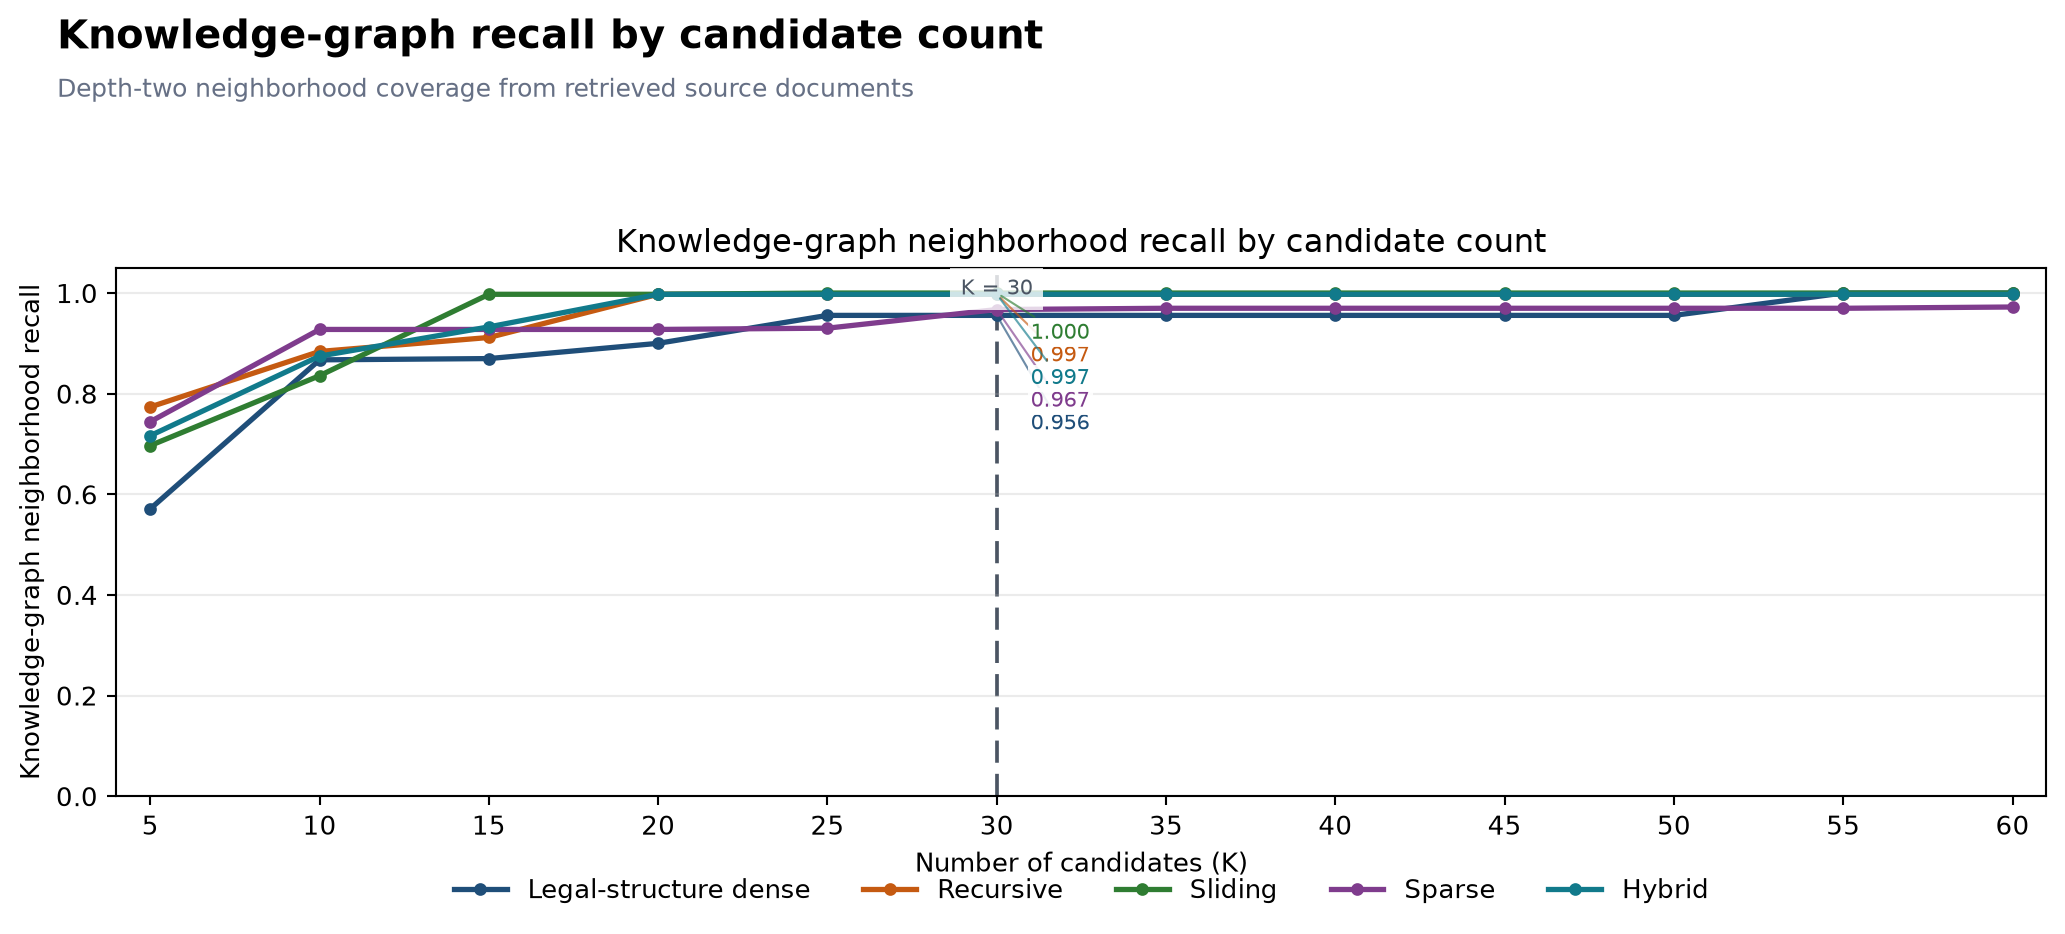
\includegraphics[width=\textwidth,height=0.44\textheight,keepaspectratio]{images/experiments/legal_revision/final_eda/kg-expanded-full-recall-sweep.png}
\caption{\emph{Knowledge-graph recall} menurut jumlah kandidat untuk konfigurasi \emph{legal}}
\label{fig:legal-revision-kg-sweep-updated}
\end{figure}

Gambar~\ref{fig:legal-revision-kg-sweep-updated} memperlihatkan kenaikan \emph{coverage}
\emph{neighborhood} ketika \emph{cutoff} bertambah. \emph{Recursive}, \emph{Sliding}, dan \emph{hybrid} mendekati penuh
lebih cepat daripada \emph{dense}, sehingga traversal \emph{graph} dapat memperluas jangkauan dokumen
meskipun \emph{context reference} langsung belum seluruhnya berada pada \emph{ranking} awal.

\begin{figure}[H]\centering
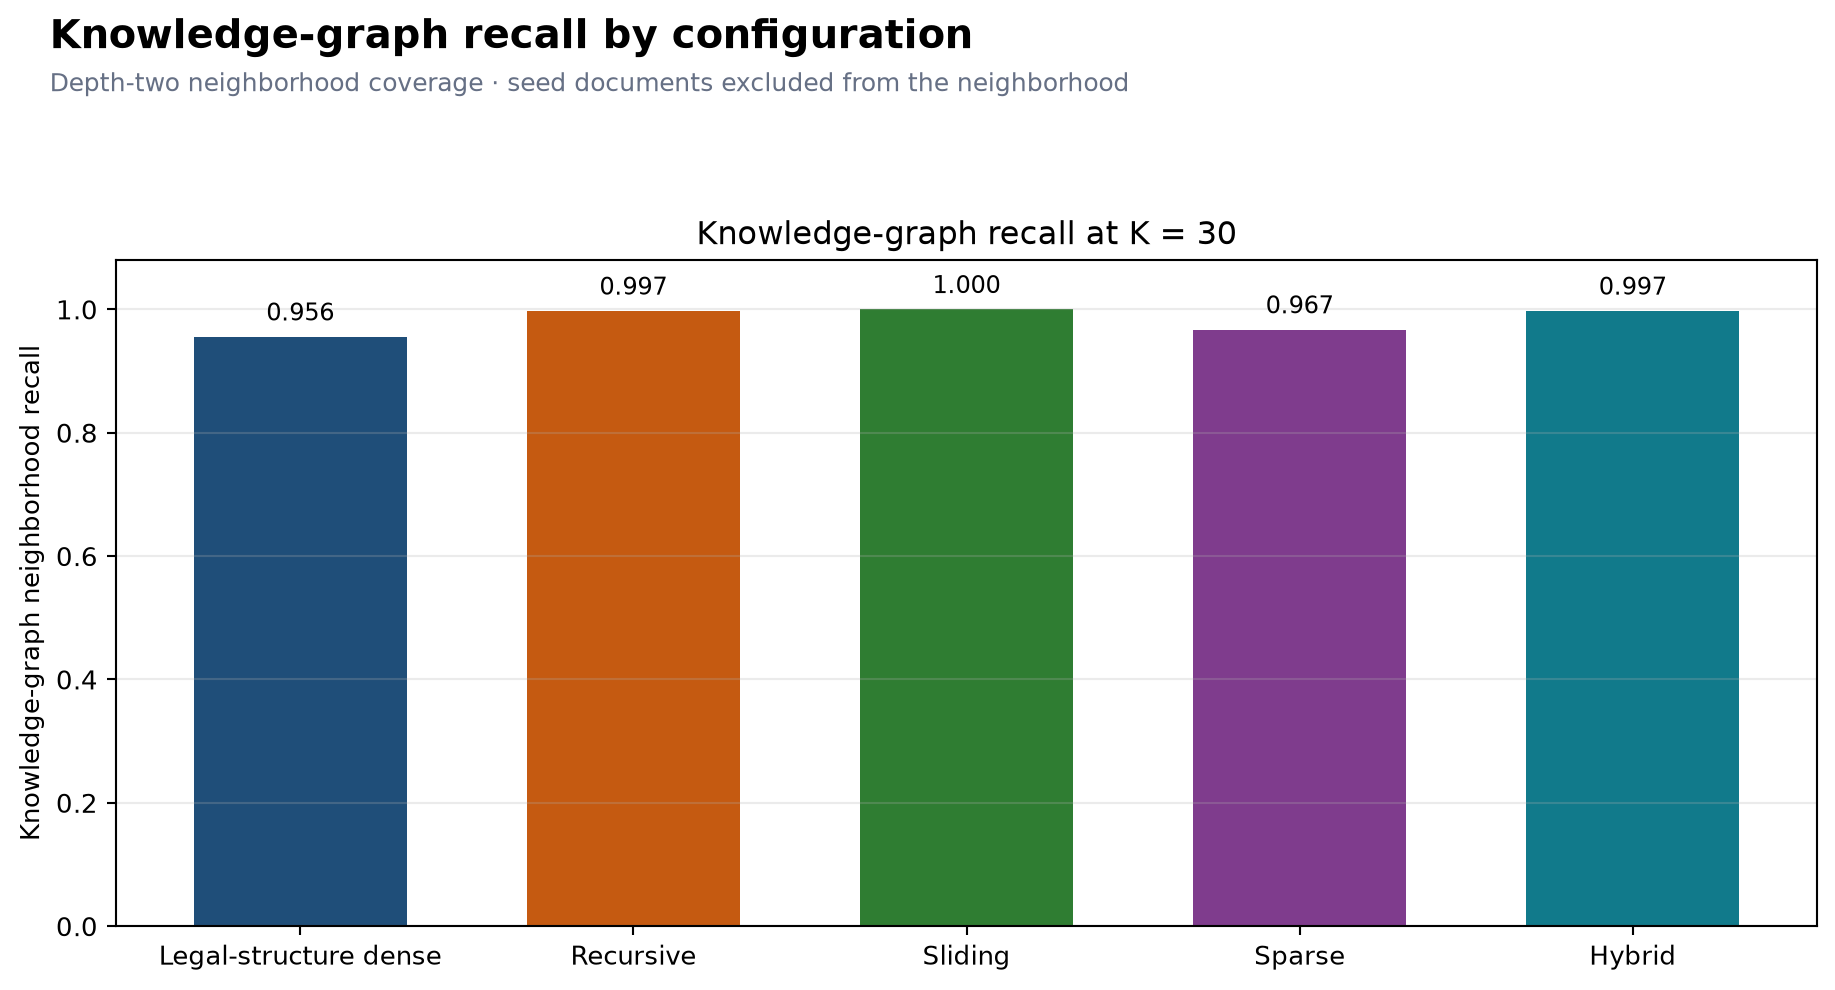
\includegraphics[width=\textwidth,height=0.44\textheight,keepaspectratio]{images/experiments/legal_revision/final_eda/kg-expanded-full-recall-k30.png}
\caption{\emph{Knowledge-graph recall} untuk konfigurasi \emph{legal} pada \(K = 30\)}
\label{fig:legal-revision-kg-k30-updated}
\end{figure}

Pada Gambar~\ref{fig:legal-revision-kg-k30-updated}, \emph{Sliding} mencapai 1,0000,
\emph{Recursive} dan \emph{hybrid} 0,9975, \emph{sparse} 0,9672, dan \emph{dense} 0,9556. Perbedaan terhadap
\emph{recall} langsung menunjukkan bahwa \emph{graph} menilai perluasan dokumen, bukan ketepatan
\emph{context reference} pada setiap posisi kandidat.

\subsection{Kesimpulan Eksperimen \emph{Legal}}
\label{subsec:legal-revision-conclusion-updated}
\label{subsec:legal-revision-conclusion}

\emph{Sliding} dan \emph{Structure-aware} \emph{sparse} ditetapkan sebagai \emph{baseline} untuk \emph{chunker} dan \emph{indexer}.
\emph{Legal-structure} \emph{dense} mengalahkan \emph{baseline} \emph{Sliding} sebesar 0,0509 \emph{recall} dan \emph{baseline}
\emph{sparse} sebesar 0,0473 \emph{recall}. \emph{Hybrid} memberikan \emph{MRR} tertinggi, yaitu 0,5439, tetapi
\emph{dense} tetap memberi \emph{coverage} \emph{context reference} tertinggi. Pada \emph{generation}, \emph{correctness}
tertinggi berada pada \emph{Legal-structure} \emph{dense}, sedangkan \emph{faithfulness} tertinggi berada pada
\emph{hybrid}. Eksperimen \emph{KG} menunjukkan bahwa \emph{coverage} \emph{neighborhood} dapat hampir penuh pada
beberapa konfigurasi walaupun \emph{recall} langsung berbeda. Dengan demikian, \emph{recall} context
\emph{reference} menjadi dasar pemilihan konfigurasi, metrik \emph{precision}, \emph{MRR}, dan \emph{NDCG} menjadi
diagnosis urutan kandidat, serta \emph{knowledge-graph recall} menjadi ukuran tambahan untuk
jangkauan dokumen terhubung.
